\documentclass[nochap]{apuntes}

\usepackage{hyperref}

\usepackage{tikztools}
\usepackage{fastbuild}
\usepackage{tikz-3dplot}

\usepackage{tikz}
\usepackage{graphicx}
\usepackage{latexsym, amsfonts, amsmath, amssymb, amscd, epsfig,amsthm}
\usepackage{enumitem}
\usepackage{natbib}
\usepackage[nottoc]{tocbibind}
\usepackage{fancysprefs}

\usepackage{listings}
\lstset{
    language=R,
    basicstyle=\ttfamily
}

\usepackage{caption}


\definecolor{codegreen}{rgb}{0,0.6,0}
\definecolor{codegray}{rgb}{0.5,0.5,0.5}
\definecolor{codepurple}{rgb}{0.58,0,0.82}
\definecolor{backcolour}{rgb}{0.95,0.95,0.92}

\lstdefinestyle{mystyle}{
    backgroundcolor=\color{backcolour},
    commentstyle=\color{codegreen},
    keywordstyle=\color{magenta},
    numberstyle=\tiny\color{codegray},
    stringstyle=\color{codepurple},
    basicstyle=\footnotesize,
    breakatwhitespace=false,
    breaklines=true,
    captionpos=b,
    keepspaces=true,
    numbers=left,
    numbersep=5pt,
    showspaces=false,
    showstringspaces=false,
    showtabs=false,
    tabsize=2
}



\input xy
\xyoption{all} %%!!
\usetikzlibrary{calc, intersections}
\author{Víctor de Juan}
\date{2014/2015 2º cuatrimestre}

\renewcommand*{\arraystretch}{1.5}
\title{Estadística II}
\precompileTikz

\begin{document}


\pagestyle{plain}
\maketitle

\tableofcontents
\newpage

% -*- root: ../EstadisticaII.tex -*-
\section{Introducción}
Se presentan apuntes de Estadística II, tomados de la clase dada por José Berrendero.

El profesor nos facilita unas diapositivas a las que se harán referencia alguna vez.

\subsection{Vectores aleatorios}


Sea $X = (X_1, \dots , X_p)'$ un vector aleatorio p-dimensional.


\begin{defn}[Esperanza]
	Definimos la esperanza como el vector de medias, es decir:
	\[
	\mathbb{E}(X) = μ = (μ_1,\dots,μ_p)'
	\]
	donde $μ_i = \mathbb{E}(X_i)$.
\end{defn}


\paragraph{Propiedades:}
\begin{enumerate}
\item $\mathbb{E}(X+c) = \mathbb{E}(X)+c$.
\item Sea A una matriz cuadrada de dimensión $n\times p$ siendo $p$ la dimensión de $X$ \[\mathbb{E}(AX) = A\mathbb{E}(X)\]

\end{enumerate}



\begin{defn}[Covarianza]
\[\sigma_{i,j} = \cov{X_i,X_j} = \mathbb{E}\left((X_i-\mathbb{E}(X_i))(X_j-\mathbb{E}(X_j))\right) = \mathbb{E}(X_i X_j)-\mathbb{E}(X_i)\mathbb{E}(X_j)\]

Dos propiedades importantes de la covarianza son:

\begin{enumerate}
\item $\cov{X,X}= \var{X}$
\item $\cov{X,Y}=\cov{Y,X}$
\end{enumerate}

\end{defn}

Al tener varias variables, ya no podemos hablar de varianzas. Definimos el correspondiente p-dimensional de la varianza.


\begin{defn}[Matriz de covarianzas]
	Llamamos $\var{X} = Σ$ a la matriz de covarianzas, cuya posición $(i,j)$ es $σ_{ij} = \cov{X_i,X_j}$.


	Curiosidades:

	\begin{itemize}
		\item Por la definición de covarianza, la diagonal de esta matriz es el vector p-dimensional cuya entrada $i$ es la varianza de $X_i$.
		\item Es una matriz \textbf{simétrica} ya que $\cov{X_i,X_j} = \cov{X_j,X_i}$
	\end{itemize}

	Además: \[\var{X} = \mathbb{E}[(X-μ)(X-μ)'] = \mathbb{E}(XX')-μμ'\]

\end{defn}

Vamos a demostrar esta útlima afirmación.

\begin{proof}
\[
\var{X}=\mathbb{E}\left((X-\mu)(X-\mu)'\right) = \mathbb{E}(XX'- \mu X' - X \mu'+\mu \mu')=
\]
\[
\mathbb{E}(XX')-\mathbb{E}(\mu X')-\mathbb{E}(X\mu')+\mathbb{E}(\mu \mu')= \mathbb{E}(XX')-\mu \mathbb{E}(X')-\mu' \mathbb{E}(X)+\mu\mu'=
\]
\[
 \mathbb{E}(XX')-\mu \mu'-\mu' \mu+\mu \mu' = \mathbb{E}(XX')-\mu \mu'=\Sigma
\]
\end{proof}

\paragraph{Propiedades:}

Sea $X$ un vector aleatorio p-dimensional, $A$ una matriz $n\times p$ y $b∈ℝ^n$

\begin{enumerate}
\item $\var{AX+b} = \mathbb{E}\left[ A(X-\mu)(X-\mu)'A' \right]=A \Sigma A'$.
\begin{proof}
\[
\var{AX+b} = \mathbb{E}\left[ (AX+b-A\mu-b)(AX+b-A\mu-b)' \right] =
\]
\[
 =\mathbb{E}\left[ (AX-A\mu)(AX-A\mu)' \right] = \mathbb{E}\left[A(X-\mu)(X-\mu)'A'\right] = A\mathbb{E}\left[(X-\mu)(X-\mu)'\right]A' =
 \]
 \[
 =A \Sigma A'
\]
\end{proof}
\label{propiedades:esperanzaYvarianza}

\subitem Con esta propiedad podemos deducir más fácilmente expresiones como $\var{X_1 - X_2}$ de la siguiente manera:
\[\var{X_1 - X_2} = (1,-1) \begin{pmatrix}σ_1^2&σ_{12}\\ σ_{21} & σ_2^2\end{pmatrix} \begin{pmatrix}1\\-1\end{pmatrix} = σ_1^2+σ_2^2 - 2σ_{12}\]

\item Si recordamos, $\var{X} > 0$. La versión matricial dice $Σ$ es semidefinida positiva.
\begin{proof}
Sea $a_i\in ℝ$ y $X = (X_1,\dots X_n)$ un vector aleatorio.

\[
0 ≤ \var{\sum_{i=1}^p a_iX_i} = \var{a'X}
\]

Por la propiedad anterior, tenemos: \[ \var{a'X} = a'Σa\], con lo que $Σ$ tiene que ser semidefinida positiva.
\end{proof}

\subitem Si $Σ$ no es definida positiva, $\implies \exists a\in ℝ^p \tq a'Σa = 0 \implies V(a'X) = 0 \implies \exists c\in ℝ \tq P(a'X = c) = 1$. Si esto se da el vector $X$ toma valores con probabilidad 1 en un subespacio de dimensión inferior a p. En el caso de $p=2$, las variables se situarían sobre una recta.

\item Sea $\vec{Y}$ un vector aleatorio $\vec{Y}\inℝ^p$con matriz de covarianzas $Σ$, distribuido normal-multidimensionalmente. Sean $A\vec{Y}$ y $B\vec{Y}$ 2 combinaciones lineales, con $A\in ℝ^q\times ℝ^p$ y $B\in ℝ^r\times ℝ^p$. Entonces:
\label{propiedad:CovCombinacionLineal}
\[\cov{A\vec{Y},B\vec{Y}} = AΣB' = BΣA'\]

\begin{proof}
\[\begin{pmatrix}A\vec{Y}B\vec{Y}\end{pmatrix} = (A,B)' \vec{Y}\equiv N_{q+r}\left(\begin{pmatrix}Aµ\\Bµ\end{pmatrix} , \begin{pmatrix}A\\B\end{pmatrix}Σ\begin{pmatrix}A'&B'\end{pmatrix} \right)
\]

Desarrollando la matriz de covarianzas: \[
\begin{pmatrix}A\\B\end{pmatrix}Σ\begin{pmatrix}A'&B'\end{pmatrix} =
\begin{pmatrix}
AΣA' & AΣB' \\ BΣA' & BΣB'
\end{pmatrix}
\]

Y la covarianza es cualquiera de los elementos que no está en la diagonal (que como es simétrica, deberían ser iguales)
\end{proof}

\end{enumerate}


\subsection{Función característica}
La función característica de un vector aleatorio $X$ es:

\[
\phi_X(t)=\mathbb{E}(\exp^{it'X})\; t\in ℝ^p
\]

\paragraph{Propiedades:} Lo interesante de esta función (como pasaba en el caso unidimensional) es lo siguiente:

\begin{prop} Sean X e Y dos vectores aleatorios:
\[
\phi_X(t)=\phi_Y(t) \Leftrightarrow X \stackrel{d}{=} Y
\]

\end{prop}


\begin{prop}[Mecanismo de Cramer-Wold]
\[a'X \overset{d}{\equiv} a'Y, \; ∀a\in ℝ^p \dimplies X \overset{d}{=} Y\]
\end{prop}

\begin{proof}
\paragraph{$\implies$} es trivial.


\paragraph{$\impliedby$} se demuestra utilizando funciones características y tomando  $t = 1$.
\end{proof}

También se cumple que:

\[X_n \convs[d] X  \dimplies a'X_n \convs[d] a'X\; ∀a∈ℝ^n\]


\subsection{Normal multivariante}

Habiendo definido lo que es un vector aleatorio, vamos a definir la distribución normal multivariante, que aparecerá continuamente a lo largo del curso.

\begin{defn}[Normal p-dimensional]El vector aleatorio $X$ es normal p-dimensional  con vector de medias μ y vector de covarianzas Σ si tiene densidad dada por:
\[
f(x) = |Σ|^\frac{-1}{2}(2π)^{\frac{-p}{2}}exp\left\{ -\frac{1}{2}(x-μ)'Σ^{-1}(x-μ) \right\}\; x∈ℝ^p
\]
\label{def:Normal_multivariante}


\paragraph{Notación:} $X \equiv N_p(μ,Σ)$ significa: $X$ es normal p-dimensional con media μ y matriz de covarianzas Σ.
\end{defn}

\begin{prop}
Sea $\vec{X}\in ℝ^p$ un vector aleatorio.

\[\vec{X} \sim N_p(µ,Σ) \implies ∀\vec{a}\in \real^p, \vec{a}\vec{X}' \sim N_1(\vec{a}\vec{µ},\vec{a}Σ\vec{a}')\]
\end{prop}

\begin{proof}

Que la media y la varianza son esas, está calculado anteriormente en \ref{propiedades:esperanzaYvarianza}.

Lo de que sean una normal, \href{https://en.wikipedia.org/wiki/Normally_distributed_and_uncorrelated_does_not_imply_independent}{Wikipedia}


\end{proof}


Vamos a profundizar en esta definición porque es clave, como veremos más adelante en la \fref{sec:incorrnotindep} entre otras.

Sean \[X_1 \equiv N(0,1)\;\; X_2 = N(0,2)\] ¿El vector $\vec{X}= (X_1,X_2)$ cumple $\vec{X_2}\sim N_2 (µ,Σ)$?

\begin{prop}
\label{prop:NormalidadConjuntaIncorrelacionIndependencia}
Sean $X_i \sim N(µ_i,σ_i)$
\begin{itemize}
	\item $X_i$ independientes \textbf{entonces} $\vec{X} = (X_1,...,X_n) \sim N_n(µ,Σ)$
	\subitem Al ser independientes son incorreladas y por tanto la matriz de covarianzas será diagonal.
	\item $\corr{X_i,X_j} = 0$ y $\vec{X} = (X_1,...,X_n) \sim N_n(µ,Σ)$ \textbf{entonces} son independientes.
\end{itemize}
\end{prop}


\begin{example}
Vamos a ver un ejemplo en dimensión 2 para ilustrar cómo reconocer si un conjunto de datos tiene una distribución normal.

Sean $μ = (0,0)'$ y $Σ = \begin{pmatrix} λ_1 & 0 \\ 0 & λ_2 \end{pmatrix}$

Vamos a ver sus conjuntos de nivel tomando:

\[(X_1,X_2) Σ^{-1} (X_1,X_2)' = cte \implies \frac{x_1^2}{λ_1} + \frac{x_2^2}{λ_2} = cte\]


Dependiendo de los valores de $λ_1,λ_2$ tendremos casos distintos.

\begin{itemize}
	\item Si $λ_1 = λ_2$, entonces tendremos circunferencias.
	\item $λ_1 ≠ λ_2$ entonces tendremos elipses.
	\subitem
	Estas elipses tendrán como eje mayor uno de los 2 ejes, ya que las variables son independientes ($\cov{X_1,X_2} = 0$).
	\subitem Si por el contrario, $Σ$ no fuera diagonal, entonces las variables no serían independientes y tendríamos una correlación entre las variables provocando que el eje mayor de la elipse fuera una recta que no corresponde con ninguno de los ejes.
\end{itemize}


Para más información consultar las transparencias de Berrendero, en las que hay un ejemplo.

\end{example}


\subsection{Incorreladas no implica independientes}
\label{sec:incorrnotindep}
\textcolor{gray}{Esta sección sale de \href{https://en.wikipedia.org/wiki/Normally_distributed_and_uncorrelated_does_not_imply_independent}{Wikipedia}}


\begin{defn}[Correlación]
Sean $X,Y$ dos variables aleatorias. Se define el coeficiente de correlación:
\[\rho_{X,Y}=\corr{X,Y}={\cov{X,Y} \over \sigma_X \sigma_Y}\]

\paragraph{Curiosidades:}

\begin{itemize}
	\item $\rho_{X,Y} ∈ [-1,1]$ Así, podemos comparar todas las correlaciones independientemente de las variables.
	\item 2 variables se llaman \concept{Variables incorreladas} si y sólo si su coeficiente de correlación es $0$.
	\item Obviamente, $\cov{} = 0 \implies \corr{} = 0$
\end{itemize}
\end{defn}


\paragraph{¿Incorrelación implica independencia?}

En general es un problema muy interesante y útil la independencia o no de variables y la correlación es algo fácil de calcular, pero \textbf{incorrelación \underline{NO} implica independencia}. Esto sólo ocurre en algunos casos.

\begin{itemize}
	\item Cuando las variables $X,Y$ son Bernoulli, entonces incorrelación si implica independencia.\footnote{Esto para el curso da igual, pero es interesante de saber}
	\item Si $\vec{X} = (X_1,X_2) \sim N_2(µ,Σ)$ y $\corr{X_1,X_2} = 0$, entonces $X_1$ es independiente de $X_2$.

	\subitem La condición de $\vec{X} \sim N_2(µ,Σ)$ es muy importante. Si sólo tuviéramos $X_i \sim N_1(µ,σ)$, entonces incorrelación \textbf{no} implica independencia.

	Es por ello que este comentario se sitúa después de la definición de normal multivariante (\fref{def:Normal_multivariante})
\end{itemize}

\begin{prop}
Sea $\vec{Y}$ un vector distribuido normalmente.

\textbf{Entonces:} un vector cualquiera $\vec{X}$ se distribuye normalmente si lo podemos escribir en la forma $A\vec{Y}$, para una matriz A.
\end{prop}

\begin{proof}
Nos lo creemos del correo electrónico.
\end{proof}



\subsection{Estandarización multivariante}


Al igual que en el caso unidimensional, nos interesaría poder transformar una normal de media $μ$ y varianza $Σ$ en una $N(0,1)$. A continuación vamos a ver ese proceso con una normal multivariante.


\begin{prop}[Estandarización multivariante] Si $X \equiv N_p(\mu, \Sigma)$ y definimos $Y = \Sigma^{-1/2}(X-\mu)$, entonces $Y_1,...,Y_p$ son i.i.d. N(0,1).\end{prop}

\begin{proof}
Sabemos por definición que:
\[
f_X(x)=\abs{\Sigma}^{-1/2}(2\pi)^{-p/2} exp \left( -\frac{1}{2}(x-\mu)' \right)
\]

Vamos a aplicar un cambio de variable en la fórmula de la densidad:

Despejando de $Y = h(X)= \Sigma^{-1/2}(X-\mu)$, obtenemos que $\Sigma^{1/2}Y+\mu=h^{-1}(Y)=X$.

Y ahora cogemos el Jacobiano de $h^{-1}(Y)=X$ que será $\Sigma^{1/2}$ ($\mu$ es una constante e Y es la variable).

También hay que considerar la exponencial de la fórmula de la densidad, ahi hacemos el cambió de variable de:

$$e^X \text{ por } e^{h^{-1}(Y)}=e^{\Sigma^{1/2}Y+\mu}$$

Y el Jacobiano sería $e^{\Sigma^{1/2}Y}$:


Por tanto nos quedaría:
\[
f(X) = f(h^{-1}(Y))·\abs{Jh(x)} = \abs{\Sigma}^{-1/2}(2 \pi)^{-p/2} \exp\left(-\frac{1}{2}(\Sigma^{-1/2}Y+\mu-\mu)'  \right) \exp\left( \Sigma^{1/2}Y \right) \Sigma^{1/2}  =
\]
\[
= \abs{\Sigma}^{-1/2}(2 \pi)^{-p/2} \exp\left(-\frac{1}{2}(\Sigma^{-1/2}Y)' \right) \exp\left( \Sigma^{1/2}Y \right) \abs{\Sigma}^{1/2} =
\]
\[
\abs{\Sigma}^{-1/2}(2 \pi)^{-p/2} \exp\left(-\frac{1}{2}(Y'\Sigma^{-1/2}\Sigma^{1/2}Y \right) \abs{\Sigma^{1/2}} = (2 \pi)^{-p/2} \exp\left(-\frac{1}{2}(Y'Y) \right)
\]
\end{proof}



Vamos a ver un ejemplo para profundizar en la distribución.
\begin{example}
Definimos el siguiente vector aleatorio: $X = (X_1,X_2,X_3)' \equiv N_3(\mu, \Sigma)$ con:

\[
\mu=
\left(
\begin{array}{c}
0\\
0\\
0
\end{array}
\right) \text{,       }
\Sigma=
\left(
\begin{array}{ccc}
7/2& 1/2& -1 \\
1/2& 1/2& 0 \\
-1& 0& 1/2
\end{array}
\right)
\]

\ppart Calcula las distribuciones marginales $X_i \equiv N(\mathbb{E}(X_i), \var{X_i})$:

$X_1\equiv N(0, 7/2)$

$X_2\equiv N(0, 1/2)$

$X_3\equiv N(0, 1/2)$

Para calcular estos valores solo hace falta mirar los datos que nos da el problema, el vector de medias $\mu$ y la matriz de covarianzas $\Sigma$:

\[
\Sigma=\left(
\begin{array}{ccc}
\var{X_1}& \sigma_{1,2}& \sigma_{1,3} \\
\sigma_{2,1}& \var{X_2}& \sigma_{2,3} \\
\sigma_{3,1}& \sigma_{3,2}& \var{X_3}
\end{array}
\right)
\]

\[
\mu=
\left(
\begin{array}{c}
\mathbb{E}(X_1)\\
\mathbb{E}(X_2)\\
\mathbb{E}(X_3)
\end{array}
\right)=
\left(
\begin{array}{c}
\mu_1\\
\mu_2\\
\mu_3
\end{array}
\right)
\]

\ppart Calcula la distribución del vector $(X_1,X_2)'$:

Este vector sigue una distribución normal que puede obtener de las matriz $\Sigma$ y el vector de medias $\mu$:
\[
\left(
\begin{array}{c}
X_1\\
X_2
\end{array}
\right)
\equiv N_2\left[
\left(
\begin{array}{c}
0\\
0
\end{array}
\right)
\text{, }
\left(
\begin{array}{cc}
7/2& 1/2 \\
1/2 & 1/2
\end{array}
\right)
\right]
\]

\ppart ¿Son $X_2$ y $X_3$ independientes?

Sí son independientes ya que la covarianza entre ambas variables es 0. La covarianza entre $X_2$ y $X_3$ es el elemento de la fila 3 y la columna 2 de la matriz de covarianzas $\Sigma$, (que al ser $\Sigma$ simétrica coincide con el elemento de la fila 2 y la columna 3).

\ppart ¿Es $X_3$ independiente del vector $(X_1, X_2)'$?

No son independientes ya que el vector de covarianzas entre ambas variables no es 0. Como en el caso anterior, tomamos como el elemento que ocipa la fila 3 y las columnas 1 y 2, es decir, el vector $(-1,0)$, que al no ser idénticamente nulo, concluimos que $X_3$ no es independiente del vector $(X_1,X_2)$


\ppart Calcula la  distribución de la variable aleatoria $(2X_1-X_2+3X_3)$.

Procedemos de la siguiente manera:

\[
(2X_1-X_2+3X_3)=(2,-1,3)\left(
\begin{array}{c}
X_1\\
X_2\\
X_3
\end{array}
\right)\equiv
N\left( 0,  \right)
\]

\end{example}



\subsection{Distribuciones condicionadas}

\begin{prop}

Sea $X=(X_1, X_2)$ con $X_1∈ℝ^p$ y $X_2∈ℝ^{p-q}$.

\begin{gather*}
µ = (µ_1, µ_2)\\
Σ = \left(\begin{array}{c|c} Σ_{11} & Σ_{12} \\\hline Σ_{21} & Σ_{22}
\end{array}\right)
\end{gather*}
\label{form::EspVarCondicionada}


\textbf{entonces: }  $X_2 | X_1 \sim N_{p-q}\left(µ_{2.1},Σ_{2.1}\right)$, donde

\begin{equation}
µ_{2.1} = µ_2 + Σ_{2.1}Σ_{11}^{-1}(X_1 - µ_1) = \esp{X_2|X_1}
\end{equation}

\begin{equation}
	Σ_{2.1} = Σ_{22} - Σ_{21}Σ_{11}^{-1} Σ_{12} = \var{X_2 | X_1}
\end{equation}

\end{prop}

\begin{proof}
Definimos $X_{2.1} = X_2 - Σ_{21}Σ_{11}^{-1}X_1$.

\[
\begin{pmatrix}
X_1\\
X_{2.1}
\end{pmatrix} =
\begin{pmatrix}
I &| &0\\
\hline
- Σ_{21}Σ_{11}^{-1}  &| &I
 \end{pmatrix}
\]

Como es una combinación lineal de $(X_1,X_{2.1})'$, entonces $X_{2.1}$ es normal multivariante.

Vamos a calcular la media y la matriz de covarianzas de $X_{2.1}$

$X_{2-1} = N\left( µ_2-Σ_{21}Σ_{11}^{-1}µ_1 , \begin{pmatrix} Σ_{11} &|&0\\\hline 0&|&Σ_{2.1} \end{pmatrix} \right)$

Donde las covarianzas se calculan: $AΣA'$, siendo $A$ la matriz de la combinación lineal, es decir:

\[
A=\begin{pmatrix}
I &| &0\\
\hline
- Σ_{21}Σ_{11}^{-1}  &| &I
 \end{pmatrix}
\]



\paragraph{Conclusiones:}

\begin{itemize}
	\item $X_1$ es independiende de $X_{2.1}$
	\item $X_{2.1}$ es normal, con media y varianza calculadas anteriormente.
	\subitem $X_{2.1}|X_1$, al ser independientes, también se distribuye normalmente, con los mismos parámetros.
	\item Dado $X_1$, los vectores $X_{2.1}$ y $X_2$  difieren en el vector constante $Σ_{21}Σ_{11}^{-1}X_1 \implies X_2|X_1 = N\left( µ_{2.1}, Σ_{2.1} \right)$
\end{itemize}

\end{proof}

\begin{example}
Vamos a considerar $X_1, X_2$ como escalares, para entender la proposición. Este ejemplo le surgió a un investigador que quería predecir la estatura de los hijos en función de la de los padres (que no padres y madres, sólo padres).


\[
\begin{pmatrix}
X\\Y
\end{pmatrix} \equiv N_2\left( \begin{pmatrix} µ_x \\ µ_y \end{pmatrix}, \begin{pmatrix}
σ_x^2&σ_{xy}\\σ_{xy}&σ_y^2
\end{pmatrix} \right)
\]
Definimos \[\gor{Y} = \esp{Y|X} = µ_y + \frac{σ_{xy}}{σ_x^2}(x-µ_x)\]. La esperanza de la altura del hijo condicionada a la altura del padre será la media de las alturas de los hijos corregida por un factor en el que influye la diferencia de altura del padre con respecto a su media. Es de esperar que si Yao Ming tiene un hijo, sea más alto que la media.

El factor de corrección $\frac{σ_{xy}}{σ_x^2}$ es importante y no me he enerado bien de dónde sale.

Ahora vamos a calcular $\var{Y|X} = σ_{y}^2 - \frac{σ_{xy}^2}{σ_x^2} = σ_y^2 \left( 1- \rho^2\right)$ donde $\rho = \frac{σ_{xy}^2}{σ_x^2σ_y^2}$, el coeficiente de correlación.

Ha dicho algo así como \textit{La única relación que puede existir entre 2 variables normales es una relación lineal.}


Este coeficiente de correlación aparece también en la expresión de la esperanza. Vamos a verlo:

 \[\gor{Y} = µ_y + \frac{σ_{xy}}{σ_x^2}(x-µ_x) \dimplies \frac{\gor{Y}-µ_y}{σ_y} = \frac{σ_{xy}}{σ_xσ_y}\frac{x-µ_x}{σ_x}\]

 Es decir:

 \[
\frac{\gor{Y}-µ_y}{σ_y} = \rho \frac{x-µ_x}{σ_x}
 \]

Aplicado a la estatura de los hijos respecto de los padres, se interpreta como: ``Si un padre es muy alto, su hijo será alto pero no destacará tanto como el padre''. Este fenómeno lo definió como \concept{Regresión a la mediocridad}.

\end{example}

\begin{defn}[Homocedásticidad]\label{defn::Homocedasticidad}
Sea $X=(X_1 ,X_2)$ con $X_1∈ℝ^p$ y $X_2∈ℝ^{p-q}$. Entonces son vectores \textbf{homocedásticos} $\dimplies Σ_{2.1}$ es constante.

Ya veremos más adelante este concepto con mayor detalle.
\end{defn}


\begin{example}

Ahora vamos a ver un par de ejemplos numéricos:

Sea \[\begin{pmatrix}X,Y\end{pmatrix} \equiv N_2 \left( \begin{pmatrix}0,0\end{pmatrix}, \begin{pmatrix}10&3\\3&1\end{pmatrix} \right)\]

\paragraph{Distribución $Y|X$:}

Utilizando las fórmulas definidas en \ref{form::EspVarCondicionada} para $X_i$ unidimensionales:

\[\esp{Y|X} =  µ_{2-1} = 0 + 3·\frac{1}{10}(X-0) = \frac{3}{10}x\]
\[\var{Y|X} = Σ_{2.1} = 1-\frac{3}{10}·3 = \frac{1}{10}\]

\paragraph{Distribución $X|Y$:}

\[E(X|Y) = 3y\]
\[V(X|Y) = 1\]

Ambas son normales unidimensionales ya que $(X,Y)$ es normal multivariante.

\end{example}

\begin{example}
Sea \[\begin{pmatrix}X\\Y\end{pmatrix} \sim
N_2\left( \begin{pmatrix}1\\1\end{pmatrix}, \begin{pmatrix} 3&1\\1&2 \end{pmatrix}\right)\]

Queremos calcular la distribución de $(X+Y) | (X-Y) = 1$

Para ello, definimos 2 variables, $Z_1 = X+Y$ y $Z_2 = X-Y$, con lo que ahora tenemos que calcular $Z_2 | Z_1 = 1$

Lo primero es hallar la relación matricial entre $X,Y$ y $Z_i$

\begin{equation*}
	\begin{pmatrix}Z_1 \\ Z_2 \end{pmatrix} = \begin{pmatrix}X+Y\\X-Y\end{pmatrix} = \begin{pmatrix} 1 & 1\\1&-1 \end{pmatrix}\begin{pmatrix}X\\Y\end{pmatrix}
\end{equation*}

¿Cuáles son la esperanza y la matriz de covarianzas de el vector aleatorio $(Z_1,Z_2)$? Para ello necesitamos la matriz de la combinación lineal que ya tenemos:

\[
µ_Z = A·µ_{xy} = \begin{pmatrix}1&1\\1&-1\end{pmatrix} \begin{pmatrix}1\\1\end{pmatrix} = \begin{pmatrix} 2\\0 \end{pmatrix}
\]

\[
Σ_Z = AΣ_{xy}A' = \begin{pmatrix}1&1\\1&-1\end{pmatrix} \begin{pmatrix} 3&1\\1&2 \end{pmatrix}  \begin{pmatrix}1&1\\1&-1\end{pmatrix} = \begin{pmatrix}7&1\\1&3\end{pmatrix}
\]

Ahora ya podemos calcular la distribución como en el ejemplo anterior:

\begin{gather*}
	\esp{Z_1 | Z_2 = 1} = 2+1·\frac{1}{3}(1-0) = \frac{7}{3}\\
	\var{Z_1 | Z_2 = 1} = 7 - 1·\frac{1}{3} · 1 = \frac{20}{3}
\end{gather*}

En este caso, al ser homocedásticas (\ref{defn::Homocedasticidad}) entonces $\var{Z_1 | Z_2 = 1} = \var{Z_1 | Z_2 = n} ∀n∈ℕ$

\end{example}


\subsection{Formas cuadráticas bajo normalidad}

\begin{prop}[]
Sea $B$ una matriz simétrica e idempontente, $$Y\sim N_2(µ,σ^2I_n)$$ y \[µ'Bµ = 0 \text{  y  } p = Rg(B)\]

\textbf{Entonces: } \[\frac{Y'BY}{σ^2} \equiv \chi_p^2 \]
\end{prop}

\obs
\begin{itemize}
	\item La única matriz idempontente de rango completo es $I_n$
	\item $λ = 0,1 ∀λ$ autovalor de $B$.
	\begin{proof}
\[\left.\begin{array}{c} Bu = λu\\ Bu=B^2u = λBu = λ^2u \end{array}\right\} λu = λ^2u \implies λ=0,1\]
	\end{proof}

	\subitem Este último hecho permite calcular los grados de libertad de la distribución más fácilmente, ya que $p = Rg(B) = tr(B) = \#\{i \tq λ_i = 1\}$
\end{itemize}


\begin{lemma}[Lema de Fisher]
Sean $Y_1,..,Y_n \overset{iid}{\sim} N(µ,σ)$. Vamos a considerar el vector cuyas marginales son estas $Y \equiv (Y_1,...,Y_n) = N(µ1_n,σ^2I_n)$\footnote{$1_n = (1,1,...,1)$ n veces.}

\textbf{Entonces: } $\gor{Y}, S^2 = \frac{\sum (Y_i - \gor{Y})^2}{n-1}$ son independientes. Además,
\[\frac{(n-1)S^2}{σ^2} \equiv \chi^2_{n-1}\]

\end{lemma}

\begin{proof}
Lamentándolo mucho, la prueba será ignorada por el momento.
\end{proof}


\begin{theorem}[TCL Multivariante]
Sean $X_1,...,X_n$ vectores aleatorias independientes e idénticamente distribuidas (vec.a.i.i.d.) con $X_i \sim N(µ,Σ)$, con $Σ$ definida positiva.

\textbf{Entonces:}

\[\sqrt{n} Σ^{\frac{-1}{2}} (\gor{X_n} - µ) \convs[d] N(0,I) \dimplies \sqrt{n}(\gor{X_n}-µ) \convs[d] N_p(0,Σ)\]

La velocidad a la que $\gor{X_n}$ converge a $µ$ es del orden de $\frac{1}{\sqrt{n}}$

\end{theorem}

\begin{proof}
Lamentándolo mucho, la prueba será ignorada por el momento.
\end{proof}

% -*- root: ../EstadisticaII.tex -*-
\chapter{Contrastes no paramétricos}
\section{Introducción}
\begin{defn}[Hipótesis no paramétrica]
Hipótesis que no se formula en términos de un número finito de parámetros.\end{defn}

En este capítulo vamos a ver 3 tipos de contrastes (con diferentes test para algunos contrastes)
\begin{enumerate}
\item \textbf{Bondad de ajuste:} A partir de una muestra $X_1,...,X_n \equiv F$ de variables aleatorias independientes idénticamente distribuidas, contrastar:
\begin{itemize}
\item $H_0: F=F_0$ donde $F_0$ es una distribución prefijada.
\item $H_0: F \in \{F_{\theta} : {\theta}\in H\}$, donde H es el espacio paramétrico.
\end{itemize}
\item \textbf{Homogeneidad:} Dados $X_1,...,X_n \equiv F$ y $Y_1,...,Y_n \equiv G$ de variables aleatorias independientes idénticamente distribuidas. Contrastar $H_0: F=G$.
\item \textbf{Independencia:} Dada $(X_1,Y_1),...,(X_n,Y_n) \equiv F$ de variables aleatorias independientes idénticamente distribuidas. Contrastar $H_0: X$ e $Y$ son independientes.
\end{enumerate}


%%%%%%%%%%%%%%%%%%%%%%%%%%%%%%%%%%%%%%%%%%%%%%%%%%%%%%%%%%%%%%%%%%%%%%%%%%%%%%%%%%%%%%%%%%%%%%%%%%

\section{Contrastes de bondad de ajuste}

\subsection{Contraste $\chi^2$ de bondad de ajuste}
Consideramos una distribución totalmente especificada bajo $H_0: X_1,...,X_n \equiv F$ de variables i.i.d.

$H_0: F=F_0$ es la hipótesis nula y queremos ver que F, que es la distribución obtenida con los datos verdaderos (obtenidos empíricamente) es igual a $F_0$ que es la distribución teórica.

Vamos a definir los pasos que tenemos que seguir para comprobar si $H_0$ es cierta:
\begin{enumerate}
\item Se definen k clases $A_1,...,A_k$. En el caso del dado, los valores de cada cara.
\item Se calculan las frecuencias observadas de datos en cada clase.
\subitem \[O_i = \#\{j\tq X_j ∈ A_i\}\]
\[O_i \sim Bin\left(n,p_i = p_{H_0}(A_i)\right) \text{ es una variable aleatoria}\]
\item Se calculan las frecuencias esperadas si $H_0$ fuera cierta:
	\subitem\[\esp{F}_i = \esp{F}_{H_{0}} = np_i \text{ al ser } O_i \text{ una binomial}\]
\item Se comparan $O_i$ con $E_i$ mediante el estadístico de Pearson, para comprobar si lo observado se parece a lo esperado.

\[T = \sum_{i=1}^k \frac{(O_i - E_i)^2}{E_i}\]

\subitem Más adelante justificaremos porqué este estadístico es el utilizado. Además, el estadístico puede calcularse de otra manera:

\[
T = \sum \frac{O_i^2}{E_i} - n
\]
\item Se rechaza $H_0$ en la región crítica $R = \{ T>c\}$, donde $c$ depende del nivel de significación $α$.
\subitem $c$ se obtiene consultando en las tablas para $α = P_{H_0}(T>c)$
\end{enumerate}

Pero se nos presenta el siguiente problema, ¿Cuál es la distribución de $T$ bajo $H_0$?

\begin{theorem}[Estadístico\IS de Pearson]
El estadístico de Pearson es:
\[T = \sum_{i=1}^k \frac{(O_i - E_i)^2}{E_i} = \sum_{i=1}^k \frac{O_i^2}{E_i} - n\]

Además, bajo $H_0$ su distribución:

\[
T \convs[d] \chi^2_{k-1}
\]
\end{theorem}

\begin{proof}
\textcolor{red}{Para otro momento}
\end{proof}

\begin{example}
Tiramos un dado 100 veces y obtenemos:

\begin{tabular}{|c|c|c|c|c|c|c|}
\hline
Resultados & 1 & 2 & 3 & 4 & 5 & 6 \\
\hline
Frecuencia & 10 & 20 & 20 & 10 & 15 & 25\\
\hline
\end{tabular}

Y consideramos $H_0: p_i=\frac{1}{6} \; \forall i=1,...,6$. Es decir que el dado no está trucado y cada cara tiene la misma probabilidad ($p_i$) de salir.

¿Es cierta la hipótesis, con un nivel de confianza/significación del 95\%?


Las clases son cada uno de los posibles resultados y las frecuencias observadas se encuentran en la tabla.

Vamos a calcular el estadístico $T$ \[T = \sum_{i=1}^6 \frac{O_i^2}{E_i} - n = \frac{6}{100} (\sum O_1^2) - 100 = ... = 11\]

Ahora, consultando las tablas buscamos el valor $\chi^2_{5;0.05} = 11.07 > T = 11$, entonces no estamos en la región crítica, por lo que no podemos rechazar la hipótesis.

Al ser valores muy próximos, observamos que el p-valor\footnote{el menor nivel de confianza para poder rechazar} del contraste tendrá que ser algo mayor que $0.05$.

\end{example}







\subsubsection{Hipótesis nula compuesta}

Vamos a estudiar el siguiente problema. Sea $X_1,...,X_n \overset{}{\sim}{iid}  F$ y una hipótesis compuesta: $H_0: F\in \{ F_{\theta}, \theta\in Ω \subset ℝ^n\}$. Esta hipótesis compuesta puede ser ``los datos se distribuyen normalmente, con media y varianza desconocidas''

Los pasos a seguir son:
\begin{enumerate}
	\item Definir las clases $A_1,...,A_k$
	\item Calcular las frecuencias observadas $O_1,...,O_k$
	\item Estimamos $\theta$ por el método de máxima verosimilitud. Sea $\gor{\theta}$ el e.m.v.
	\subitem Pero para calcular las frecuencias esperadas, no tenemos una única normal. La idea intuitiva sería: hay unos parámetros que son los que mejor ajustan la distribución. ¿Cuál es la que mejor ajusta? La que tenga los parámetros estimados.
	\item Ahora ya podemos calcular las frecuencias esperadas:

	$E_i = n\gor{p_i}$ donde $\gor{p_i} = P_{\theta}(A_i)$, con $i=1,...,k$
	\item Ya podemos calcular el estadístico de Pearson:

	\[
	T= \sum_{i=1}^k \frac{(O_i - \hat{E_i})^2}{\hat{E_i}}
	\]

	\subitem ¿Qué distribución tiene este estadístico? Antes hemos visto que es una $\chi^2_{k-1}$ cuando se dan unas ciertas condiciones.

	En este caso, es de esperar que $T$ tienda a tomar valores menores que en el caso simple.

	Además, al estimar $r$ parámetros (las $r$ componentes del vector $\theta$)) se introducen $r$ nuevas restricciones sobre el vector $(O_1,...,O_r)$.

Se puede probar, \footnote{bajo ciertas condiciones de regularidad que las distribuciones que conocemos cumplen y que son demasiado complicadas de enunciar} que:

\[
	\sum_{i=1}^k \frac{(O_i - \hat{E_i})^2}{\hat{E_i}} \convs[d] \chi^2_{k-1-r}
\]

	\item Se rechaza $H_0$ en  la región crítica \[R = \{ T > \chi^2_{k-1-r}\}\]
\end{enumerate}

\begin{example}
\paragraph{Los bombardeos de Londres}

Los alemanes bombardeaban mucho a Londres durante la guerra mundial, y los ingleses querían saber si los alemanes podían dirigir los misiles, o los impactos eran aleatorios.

Para ello, alguien hizo el estudio estadístico, para contrastar la hipótesis ``los impactos son aleatorios''.

Los impactos deberían seguir una Poisson \footnote{ya que es el límite de una binomial, en la que consideramos los impactos como éxitos}. Para ello, dividió Londres en $n=576$ cuadrados, cada uno de ellos será la variable $X_i$ que debería seguir una Poisson.

La idea del contraste es: la Poisson que más se puede parecer es la que tenga de media el e.m.v. Si esa Poisson no se parece, entonces ninguna Poisson se puede parecer.



\begin{enumerate}
	\item[Clases] Los valores que toma la Poisson (recordamos que son número naturales). En este caso sólo se han definido 5, ya que la última es $>4$ \footnote{Se recomienda no definir más de 5 clases, para que la estimación no pierda demasiada información. }
	\item[Obs] $O_i = \{\#j : X_j=i\}$, por ejemplo, las frecuencias observadas de la clase $0$, es decir, $O_0 = 229$, donde ese número es el número de las $n$ regiones de Londres en donde no cayó ningún misil.
	\item[e.m.v.] El e.m.v. de una Poisson es la media muestral, con lo que $\hat{λ} = \gor{x} = 0.9323$
	\item[Esp] Calculamos las frecuencias esperadas utilizando el parámetro estimado $$\hat{E_i} = n\hat{p_i} = 576 · e^{-0.9323}\frac{(0.9323)^i}{i!}$$
	\item[T] El estadístico $\chi^2$ de Pearson es: \[T = \sum_{i=1}^k \frac{(O_i - \gor{E_i})^2}{\gor{E_i}} = 1.01 \]

	Desde esta información, ya podemos hacernos una idea de si vamos a poder rechazar. ¿Por que? Al estimar un único parámetro $T \overset{iid}{\sim} \chi^{2}_{5-1-1}$, y además $\mathbb{E}(\chi^2_k) = k$, con lo que  debería habernos salido $T=3$. Al ser un vector bastante normal, podemos ver que tiene muy poca pinta de que vayamos a poder rechazar la hipótesis nula. Al $T$ estar por debajo de $3$ no estaremos en la región crítica.

\end{enumerate}


\obs Este ejemplo se encuentra también en las transparencias, donde podemos ver los valores y algunas gráficas explicativas.
\end{example}


\subsubsection{Contrastes con $R$}
\paragraph{Hipótesis simple}
Con el siguiente código de $R$, podemos hacer el contraste de bondad de ajuste de una $\chi^2$ fácilmente.

\begin{lstlisting}[style=mystyle]
obs = c(10,20,20,10,15,25)
ls.str(chisq.test(obs))
\end{lstlisting}

Si a \textit{chisq.test} no le damos más argumentos, supondrá hipótesis simple con equiprobabilidad de $p$. Podríamos darle otro argumento, y hacer lo siguiente para el ejemplo de los misiles:

\begin{lstlisting}[style=mystyle]
res = c(seq(0,4),7)
obs = c(229,211,93,35,7,1)
n = sum(obs)
lambda = sum(res*obs)/n
prob = dpois(res,lambda)
esp = n*prob
# Se agrupan las dos ultimas clases:
obs = c(obs[1:4],sum(obs[5:6]))
prob = c(p[1:4],1-sum(p[1:4]))
esp = c(esp[1:4],n-sum(esp[1:4]))
# Codigo para el grafico de barras:
matriz = rbind(p,obs/n)
rownames(matriz) = c('Frecuencias','Poisson')
barplot(matriz,beside=TRUE,names.arg=c(0:4),legend.text=TRUE,
col=c('lightgreen','orange'))
# Test chi 2
t = chisq.test(obs,p=prob)$statistic
pvalor = 1 - pchisq(t,3)
\end{lstlisting}


%%%%%%%%%%%%%%%%%%%%%%%%%%%%%%%%%%%%%%%%%%%%%%%%%%%%%%%%%%%%%%%%%%%%%%%%%%%%%%%%%%%%%%%%%%%%%

\subsection{Kolmogorov-Smirnov}

$X_1,...,X_n \overset{iid}{\sim} F$ y $H_0 : F=F_0$, con $F_0$ totalmente especificada.

Se define la función de distribución empírica correspondiente a $X_i$ como \[F_n(x) = \frac{1}{n}\#\{ i : X_i\leq x\}\]


\begin{example}
$X_1 = 1$, $X_2 = 6$, $X_3 = 4$


\begin{defn}[Estadístico\IS de orden]

Los estadísticos de orden, consisten en ordenar la muestra y se escriben: $X_{(i)}$.

Esto significa el $X_j$ que ocupa la posición $i-esima$ cuando ordenamos de menor a mayor. Es decir, $X_{(1)} = \min\{X_j\}$ y $X_{(n)} = \max\{X_j\}$ 
\end{defn}
Es una función de distribución constante a trozos con saltos de magnitud $\frac{1}{n}$ en cada valor muestral $X_i$ (si no hay empates). En este caso, la función de distribución es $f(a) = \frac{1}{3}, a=\{1,4,6\}$

$F_n$ es un estimador de la verdadera distribución de $F$ \[F(x) = P(X\leq x)\]
\end{example}

\obs \[\# \{i: X_i \leq x\}\] ¿Qué distribución tiene esta variable aleatoria? Es una binomial con parámetros: $B(n,F(x))$ 

\[ \esp{F_n(x)} = \frac{1}{n}nF(x) = F(x)\] Vemos que la estimación es insesgada. Además,

\[\var{F_n(x)} = \frac{1}{n^2}nF(x)(1-F(x)) \convs[] 0\]

Con lo que, $F_n \convs[P] F(x)$ y decimos que es un \concept{Estimador\IS consistente}\footnote{El estimador converge al verdadero valor. En particular, acabamos de ver que es consistente \emph{débil} porque converge en \emph{probabilidad}, pero veremos que en realidad tenemos convergencia uniforme.}

¿Esto a qué viene? A entender la función de distribución empírica.

Además de la convergencia en probabilidad tenemos un resultado más potente:

\begin{theorem}[Teorema\IS Glivenco-Cantelli]
\[ ||F_n-F||_α = \sup_{x\inℝ} |F_n(x) - F(x)| \convs[c.s.] 0\]

Es decir, la función de distribución empírica converge en distribución a la real y además esa convergencia es uniforme.
\end{theorem}

\begin{proof}
La demostración se sale del temario de este curso.
\end{proof}

\paragraph{¿Cómo se hace realmente el contraste?} Si $H_0$ fuese cierta, se espera que $D_n = ||F_n - F_0||$ sea ``pequeño''. La idea es rechazar en la región crítica $R = \{D_n > c\}$ para un valor $c$ tal que $P_{H_0}(D_n > c) = α$, siendo $α$ un nivel de significación predeterminado.

Para poder calcular $P_{H_0}(D_n > c)$ necesitamos cálculos algo chungos, pero hay un resultado que nos puede ayudar mucho a resolver este problema.

\begin{lemma}
La distribución bajo $H_0$ de $D_n$ es la misma para cualquier distribución continua $F_0$

Por tanto el valor de $c$ en la región crítica es el mismo para cualquier distribución continua $F_0$ y está tabulado.
\end{lemma}


\begin{proof}
Para poder probar este lema, necesitamos una proposición:

\begin{prop}
Si una $v.a.$ tiene distribución continua $F_0$, entonces la variable aleatoria $F_0(X)\sim \mathbb{U}(0,1)$\label{prop::funcionsobredistribucioncontinua}
\end{prop}
\begin{proof}
\[
P\{F_0(x) \leq u\} \overset{?}{=} u 
\]
Hemos tomado distribuciones continuas para evitar saltos. Entonces:

$F_0 \text{ continua} \implies \exists x \tq F_0(x) = u, P\{F_0(X)\leq F_0(x)\}$

Donde:
\[
\{F_0(X)\leq F_0(x)\} = \underbrace{\{F_0(X)\leq F_0(x), X\leq x\}}_{\{X\leq x\}} \cup \{F_0(X)\leq F_0(x), X\ge x\}
\]

Vamos a estudiar cada uno de los términos:

\[\{F_0(X)\leq F_0(x), X\leq x\} = \{X\leq x\}\]
Se debe a que $X\leq x \implies F_0(X)\leq F_0(x)$

Por otro lado, el otro término:
\[\{F_0(X)\leq F_0(x), X\ge x\} = P\{F_0(X)\leq F_0(x), X>x\} = 0\]
Ya que $F_0$ es necesariamente constante entre $x$ y $X$.


\textbf{Entonces:}

\[
\{F_0(X)\leq F_0(x)\} = P\{X\leq x\} = F(x) = u
\]
\end{proof}
\obs Existe un recíproco que permite calcular otras distribuciones a partir de uniformes invirtiendo la función de distribución.


Ahora que ya tenemos esa propiedad demostrada podemos seguir con la demostración del lema.

Vamos a demostrar que $D_n = \max\{\sup_{x\in ℝ} (F_n(x) - F_0(x)),\sup_{x\in ℝ} (F_0(x) - F_n(x)) \}$

Lo hemos separado en 2 para quitarnos el valor absoluto. Aquí solo estudiaremos uno de los términos, y el otro se deja como ejercicio para el lector.

Por definición de la distribución empírica, tenemos: $x\in [X_{(i)},x_{(i+1)}), F_n(x) = \frac{i}{n}$

\textbf{Entonces:}

\[
\sup_{x\in ℝ} (F_n(x) - F_0(x)) = \max_{i=0,...,n} \sup_{x\in [X_{(i)},X_{(i+1)})} (F_n(x) - F_0(x))
\]


Ahora podemos sustituir $F_n(x)$, obteniendo
\[
 = \max_{i=0,...,n} \left( \frac{i}{n} - F_0(x_{(i)})\right) = \max \left\{0,\max_{i=0,...,n} \left( \frac{i}{n} - F_0(x_{(i)})\right)\right\}
\]

Por el otro lado obtendríamos:

\[
\sup_{x\in ℝ} (F_0(x) - F_n(x)) = ... = \max \left\{0,\max_{i=0,...,n} \left\{0, \left(F_0(X_{(i)}) - \frac{i-1}{n}\right)\right\}\right\}
\]

\textbf{Conclusión:}
\[D_n = ||F_n - F_0||_{\infty} = \max \left\{ 0, \max_{i=0,...,n} \left( \frac{i}{n} - F_0(x_{(i)})\right), \max_{i=0,...,n} \left\{0, \left(F_0(x_{(i)}) - \frac{i-1}{n}\right)\right\}\right\}\]

Es decir, $D_n$ depende de $F_0$ a través $F_0(X_{(i)})$ y, aplicando la proposición \ref{prop::funcionsobredistribucioncontinua} en $X_1,...,X_n \overset{iid}{\sim} F_0 \to X_{(1)} \leq ... \leq X_{(n)}$

Entonces: 
\[
F_0(X_1),...,F_0(X_n) \overset{iid}{\sim} \mathbb{U}(0,1) \to F_0(X_{(1)})\leq ... \leq F_0(X_{(n)})
\]


Son los estadísticos de de orden de una muestra de tamaño $n$ de v.a.i.i.d $\mathbb{U}(0,1)$ para cualquier $F_0$ continua.

\end{proof}

\begin{example}
Contrastar a nivel α=0.01 si la muestra $16,8,10,12,6$ procede de una exponencial de media $λ=11.5$

Recordamos que la media de una exponencial: $µ = \frac{1}{λ}$.

%esto está bien seguro
En este caso, $F_0(x) = 1-e^{-\frac{x}{11.5}}$.


Vamos a construir una tabla para resolverlo, llamando $D_n^+ = \{\frac{i}{n} - F_0(X_{(i)})\}$ y $D_n^- = \{F_0(X_{(i)}) - \frac{i-1}{n} \}$
\[
\begin{array}{cccccc}
X_{(i)} & \frac{i}{n} & F_0(X_{(i)}) & D_n^+ & D_n^-\\\hline
6&0.2&0.41&-0.21&0.41\\
8&0.4&0.5&-0.1&0.3 \\
10&0.6&0.58&0.02&0.18 \\
12&0.8&0.65&0.15&0.05 \\
16&1&0.75&0.25&-0.05
\end{array}\]


En esta caso, $D_n = \max\{0,D_n^+,D_n^-\} = 0.41$. Ahora, como el contraste no depende de la $F_0$ (mientras que esta sea continua), consultamos la tabla y vemos que para $n=6$ y $α=0.01$ obtenemos $c=0.669$.

\[c>D_n \dimplies 0.669 > 0.41\]

Con lo que no podemos rechazar la hipótesis.

\end{example}

\subsubsection{Contrastes Kolmogorov-Smirnov con R}
 Para el ejemplo anterior,  el código de $R$ tendríamos algo que aparecerá más adelante:

\begin{lstlisting}[style=mystyle,escapeinside={(*}{*)}]

n = 100
x = rnorm(n)
plot(ecdf(x),vertical=TRUE, do.points=FALSE)
curve(pnorm(x),-4,4add=TRUE,col=blue)

Dn= ks.test(x,pnorm)$statistic
# En esta gráfica, (*$D_n$*) es la mayor distancia vertical entre la negra (empírica) y la azul (real).

(*\begin{center}
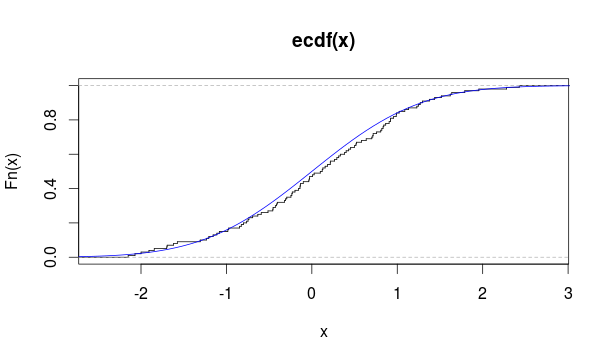
\includegraphics[scale=0.6]{img/KSR.png}
\end{center}*)



ks.test(x,pnorm) # Cierta. Obtenemos un p-valor grande (del orden de 0.7)
ks.test(x,pexp) # Falsa. Obtenemos un p-valor casi 0 (del orden de (*$10^{-16}$*))

\end{lstlisting}


\paragraph{Iteración del contraste} Es bueno repetir el contraste varias veces, ya que la generación de los datos es aleatoria. Para ello,  hay un fichero en moodle de $R$ con el proceso. En las transparencias además, está el otro ejemplo.

\subsection{Gráficos de probabilidad}

Este es otro tipo de contraste. Hemos visto cómo contrastar con una $\chi^2$. También hemos utilizado la distribución empírica.

Ahora vamos a ver cómo contrastar utilizando los cuantiles.

Tenemos:
\[
X_1,...,X_n \overset{iid}{\sim} F \implies F(X_n) \overset{iid}{\sim}\mathcal{U}(0,1) \implies F(X_{(i)}) < F(X_{(i+1)})
\]
Podemos calcular:
\[\esp{F(X_{(i)})} = \frac{i}{n+1}\]


Utilizando esta información, podemos dibujar en el eje $x$ de una gráfica los estadísticos de orden $X_{(i)}$ y en el eje $y$, ponemos: $F^{-1}\left(\frac{i}{n+1}\right)$, ya que, en media $F(X_{(i)}) \sim \frac{i}{n+1}$

Lo que esperaríamos si nuestra hipótesis de $F$ fuera cierta, es que los puntos de esa gráfica estén sobre una recta.


\begin{example}
Sea $X_1,...,X_n \overset{iid}{\sim} \underbrace{N(µ,σ^2)}_{F}$. Tomamos $\Phi \sim N(0,1)$


\[X_{(i)} \sim F^{-1}\left(\frac{i}{n+1}\right) = ... = σ\Phi^{-1}\left(\frac{i}{n+1}\right) + µ\]

Si los datos son normales, los puntos $\left( X_{(i)},\Phi^{-1}\left(\frac{i}{n+1}\right)\right)$ estarán alineados.

\end{example}

\obs Este es el tipo de contraste que se utiliza en la realidad para saber si unos datos se distribuyen normalmente o no. Hay una manera de medir esta diferencia y no hacerlo a ojo. Este test se denomina \concept{Shapiro-wilks}




\section{Contrastes de homogeneidad}
\subsection{$\chi^2$ }
Tenemos \[
\left.
\begin{array}{cc}
M_{1} \equiv X_{11} ,...,X_{1n_1} &\overset{iid}{\sim} F_1\\ 
\vdots & \vdots \\
M_{p} \equiv X_{p1} ,...,X_{pn_p} &\overset{iid}{\sim} F_p
\end{array} \right\} H_0 : F_1 = F_2 = ... = F_p 
\]

Con $M_1,...,M_p$, muestras \textbf{independientes}.

\paragraph{Proceso para el contraste}
\begin{enumerate}

\label{contraste::homogeneidad::chicuadrado}

\item Dividimos los datos en clases $A_i$ y consideramos las frecuencias observadas $O_{ij} = \{\#\text{ datos } M_j \text{ en } A_i \}$

\item Al considerar número de $M_j$, tenemos, bajo la hipótesis, que $O_{ij} \equiv B(n_j,p_i)$, con $p_i = P_{H_0}(A_i)$.

\begin{defn}[Tabla de contingencia]
\[
\begin{array}{c|ccc}
&µ_1&\cdots & µ_p \\\hline
A_1 & O_{11} & \cdots & O_{1p}\\
\vdots & \vdots & \ddots & \vdots \\
A_k & O_{k1} & \cdots & O_{kp} 
\end{array}
\]
\end{defn}

\item Las \textbf{frecuencias esperadas} bajo $H_0 \to E_{ij} = n_jp_i$.

\item Construimos el estadístico del contraste. \[\sum_j \sum_i \frac{(O_{ij} - E_{ij})^2}{E_{ij}} \convs[d] \chi^2_{p(k-1)}\]
\subitem \textit{La independencia de las $M_i$ es la que da la convergencia a la $\chi^2$.}

\subitem Dado que no conocemos $p_i$, tenemos que estimarlos a partir de los datos. ¿Cuál es el estimador? Al suponer $F_i = F_j$ podemos utilizar:

\[ \hat{p_i} = \frac{\sum_j O_{ij}}{\sum_j n_j} \implies \hat{E}_{ij} = n_j·p_i = \frac{O_{i·}}{n}O_{·j}\]

\item \textbf{Conclusión} El estadístico es: \[T = \sum_i \sum_j \frac{(O_{ij} - \hat{E}_{ij})^2}{\hat{E}_{ij}} \convs[d] \chi^2_{(p-1)(k-1)} \] 

\subitem ¿Porqué los grados de libertad? Porque al estimar perdemos un grado de libertad por cada estimación, y como aquí estamos estimando $k$ cosas, perderíamos $k$ grados de libertad. El $-1$ aparece porque no hace falta estimar $k$ sino $k-1$ ya que $\sum_i \hat{p_i} = 1$. Entonces $p(k-1) - (k-1) = (p-1)(k-1)$

Y la región de rechazo \[R = \{T>\chi^2_{(k-1)(p-1),α}\}\]

\obs También podemos construir el estadístico como:

\[
T = \sum_{i}\sum_j \frac{O_{ij}^2}{\hat{E_{ij}}} - n
\]

\begin{proof}
Se deja como ejercicio para el lector la afirmación de que el estadístico también se puede construir así.
\end{proof}
\end{enumerate}


\begin{example}

Tenemos 100 observaciones de 3 países (ESP, ITA, FRA) sobre fumadores y queremos saber si las distribuciones que siguen cada tipo de fumador son iguales.

\begin{center}


\begin{tabular}{c|ccc|c}
 & E & I & F & \#\\\hline
NF&30&15&20&65\\
FO&50&40&50&140\\
FH&20&45&30&95\\\hline
&100 & 100 & 100 & 300
\end{tabular}
¿Qué esperamos? $\to$
\begin{tabular}{c|ccc|c}
 & E & I & F & \#\\\hline
NF & 21.6 & 21.6 & 21.6 & 65 \\
FO & 46.6 & 46.6 & 46.6 & 140 \\
FH & 31.6 & 31.6 & 31.6 & 95 \\
\hline
&100 & 100 & 100 & 300
\end{tabular}
\end{center}

Ahora podemos calcular el estadístico y la región de rechazo para $α=0.05$:

\[ T = \sum_{i=1}^k \sum_{j=1}^p \frac{O_{ij}^2}{E_{ij}} -n = ... \sim 16.8\]
\[ c = \chi^2_{4,0.05} = 9.48\]

Como $T > c \implies $ Rechazamos la hipótesis.

\end{example}

\subsection{KS de homogeneidad}

Es importante destacar e este tipo de contraste que sólo es válido para \textbf{dos muestras} y sólo para \textbf{distribuciones continuas}.

Tenemos \[
\left.
\begin{array}{cc}
X_{1} ,...,X_{n} &\overset{iid}{\sim} F\\ 
Y_{1} ,...,Y_m &\overset{iid}{\sim}G
\end{array} \right\} H_0 : F = G
\]

Sean $F_n$ y $G_m$ las funciones de distribución empíricas respectivas.

Calculamos el estadístico de KS para 2 muestras:

\[
D_{n,m} = ||F_n - G_m ||_{\infty} = \sup_{a∈ℝ} | F_n(a) - G_m(a)|
\]
Bajo $H_0$, la distribución de $D_{n,m}$ no depende de $F=G$ y está tabulada (igual que en los contrastes de bondad de ajuste).

Entonces: \[R = \{ D_{n,m} > C_α\}\]
\begin{defn}[Diferencias estandarizadas al cuadrado]
\[
\frac{(O_{ij}-\hat{E_{ij}})}{\sqrt{\hat{E_{ij}}}}
\]
\end{defn} 

\section{Contrastes de independencia}

\subsection{$\chi^2$}

Sean $(X_1,Y_1),...,(X_n,Y_n) \overset{iid}{\sim} F$ con $H_0 : X,Y$ son independientes.

Los datos se suelen dar en tablas por clases, es decir: 

\[
\begin{array}{c|ccc}
&B_1&\cdots & B_p \\\hline
A_1 & O_{11} & \cdots & O_{1p}\\
\vdots & \vdots & \ddots & \vdots \\
A_k & O_{k1} & \cdots & O_{kp} 
\end{array}
\]

Una diferencia con el anterior es que que los totales no están fijados, ya que son variables.

Vamos a ver la estimación de las frecuencias esperadas $\hat{E_{ij}}$ y $E_{ij}$

\begin{align*}
E_{ij} &= n·p_{ij} = n·P(x∈A_i,Y∈B_j) \overset{H_0}{=} n·P(x∈A_i)(Y∈B_j)\\
\hat{E}_{ij} &= n \frac{O_{i·}}{n}\frac{O_{·j}}{n} = \frac{O_{i·}·O_{·j}}{n} \text{ igual que en el anterior}
\end{align*}

Ahora, calculamos $T$ y $R$ exactamente igual que en el contraste de homogeneidad $\chi^2$ \ref{contraste::homogeneidad::chicuadrado}, es decir:

\[T = \sum_i \sum_j \frac{(O_{ij} - \hat{E}_{ij})^2}{\hat{E}_{ij}} \convs[d] \chi^2_{(p-1)(k-1)} \] 

Recordamos que también podemos construir el estadístico como:

\[T = \sum_{i}\sum_j \frac{O_{ij}^2}{\hat{E}_{ij}} - n\]

Y la región de rechazo \[R = \{T>\chi^2_{(k-1)(p-1),α}\}\]


\paragraph{La diferencia entre este contraste y el de homogeneidad} es ...

% -*- root: ../EstadisticaII.tex -*-

\chapter{Regresión}
El objetivo de la regresión es predecir una/s variable/s en función de la/s otra/s.


\section{Regresión lineal}

Observamos dos variables, X e Y , el objetivo es analizar la relación existente entre ambas, de forma que podamos predecir o aproximar el valor de la variable Y a partir del valor de la variable X.

\begin{itemize}
\item La variable Y se llama variable respuesta.
\item La variable X se llama variable regresora o explicativa.
\end{itemize}

Por ejemplo:
\begin{center}
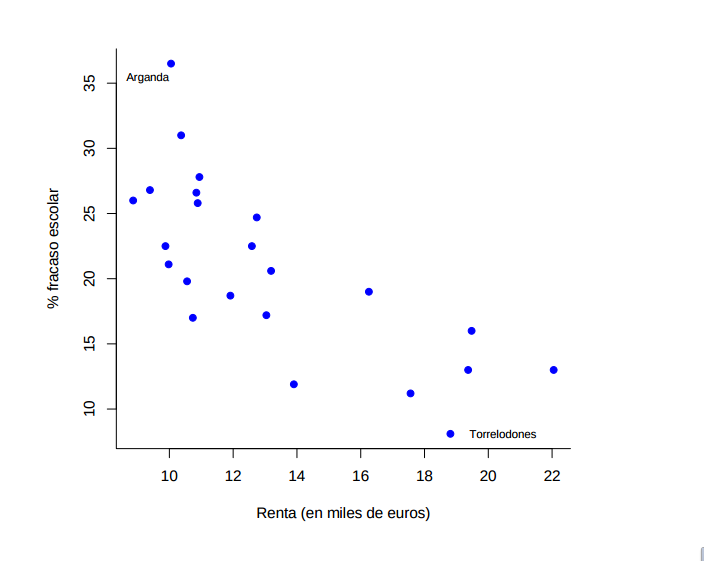
\includegraphics[scale=0.5]{img/RentaVsFracaso.png}
\end{center}

Queremos predecir el fracaso escolar en función de la renta. La variable respuesta es el fracaso escolar, mientras que la variable regresora es la renta.

\subsection{Regresión lineal simple}

Frecuentemente existe una relación lineal entre las variables. En el caso del fracaso escolar,queremos construir una recta $Y_i = β_0 X_i + β_1\; i=1,...,n$ que minimice el error.

El problema es estimar los parámetros $β_0,β_1$. Una manera de hacer esto es:

\subsubsection{Recta de mínimos cuadrados}

\begin{defn}[Recta de mínimos cuadrados]
Estimando $β_i$ por $\hat{β_i}$ obtenemos: \[\hat{Y_i} = \hat{β}_0 + \hat{β}_1 x_i\]

La recta viene dada por los valores $\hat{β_0}, \hat{β_1}$ para los que se minimiza el error cuadrático, es decir:
\[\sum_{i=1}^n \left(Y_i - \hat{Y_i}\right)^2 =  \sum_{i=1}^n \left[ Y_i - (\hat{β_0} + \hat{β_1}x_i) \right]^2\]
\end{defn}

\begin{example}
\begin{center}
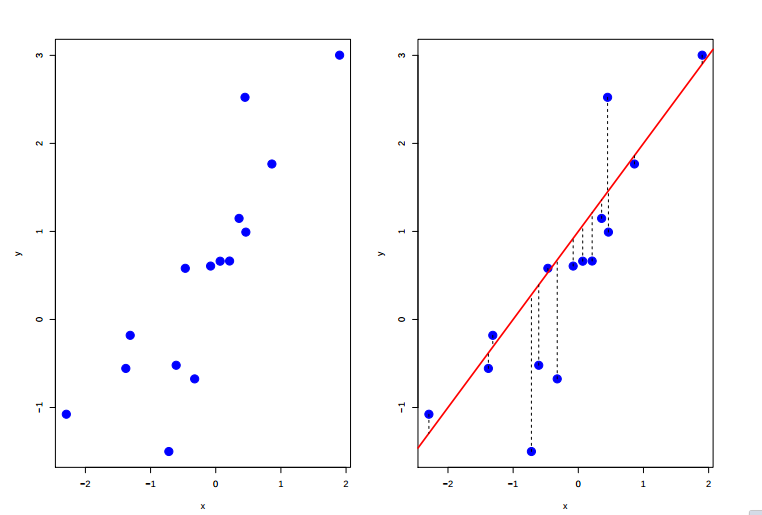
\includegraphics[scale = 0.6]{img/ejemploRectaRegresionLineal.png}
\end{center}
\end{example}

\paragraph{Cómo calcular la pendiente} de la recta de mínimos cuadrados.


Vamos a ver unas pocas maneras de calcular la recta de mínimos cuadrados.

\begin{itemize}

	\item El sistema habitual:

	\[ \hat{β_1} = \frac{\sum_{i=1}^n(x_i - \bar{x})(Y_i - \bar{Y})}{\sum_{i=1}^n (x_i - \bar{x})^2} = \frac{S_{xy}}{S_{xx}} \]
	Donde
		\[S_{xy} = \sum_{i=1}^n(x_i - \bar{x})(Y_i - \bar{Y}) \]
		\label{Ssubxx}
		Y, consecuentemente, como el avispado lector podrá imaginar
		\[S_{xx} = \sum_{i=1}^n (x_i - \bar{x})^2\]

		Es interesante darse cuenta que, siendo $S_x$ la cuasivarianza, tenemos $S_{xx} = (n-1)S_x$


	\subitem \[β_0 = \bar{Y} - \hat{β_1}\bar{x}\]

	\textbf{Entonces:}
	\[\text{recta} \equiv y - \bar{y} = \frac{S_{xy}}{S_{xx}}(x - \bar{x} ) \]

	\item Mínimos cuadrados como promedio de pendientes:
	\label{rmc::promediopendientes}
	\[
	\hat{β_1} = \frac{S_{xy}}{S_{xx}} = \sum_{i=1}^n \frac{(x_i - \bar{x})^2}{S_{xx}} \left( \frac{(Y_i - \bar{Y})}{x_i - \bar{x}} \right) = \sum_{i=1}^n ω_i \left( \frac{(Y_i - \bar{Y})}{x_i - \bar{x}} \right)
	\]

	Vemos que hemos ponderado la pendiente de cada recta que une cada punto con la media. Este peso es mayor cuanto mayor es la distancia \textbf{horizontal}.

	\item Mínimos cuadrados como promedio de respuestas:

	\[
	\hat{β_1} = \frac{\sum_{i=1}^n  (x_i - \bar{x}) (Y_i - \bar{Y})}{S_{xx}} \overset{(1)}{=} \sum_{i=1}^n \frac{x_i-\gor{x}}{S_{xx}} Y_i = \sum α_i Y_i
	\]

	$(1) \impliedby$ hemos utilizado una propiedad básica, importantísima y, a simple vista, poco (o nada) intuitiva:

	\begin{prop}
	Sea $\{x_i\},\{y_i\}$ datos de variables aleatorias.
	\[
		\sum (x_i - \gor{x}) (y_i -\gor{y}) = \sum(x_i -\gor{x})y_i = \sum (y_i - \gor{y})x_i
	\]

	\textbf{Importante:} sólo quitamos la media de una de las 2. No podemos hacer $\sum (x_i - \gor{x}) (y_i -\gor{y}) = \sum x_iy_i$, porque esto ya no es verdad.
	\end{prop}
	\begin{proof}
		\[\sum_{i=1}^n (x_i - \gor{x}) (y_i -\gor{y}) = \sum_{i=1}^n (x_i -\gor{x})y_i - \underbrace{\sum_{i=1}^n (x_i-\gor{x})\gor{y}}_{0}\]

		Vamos a ver por qué ese término es 0.
	\[\sum_{i=1}^n (x_i-\gor{x})\gor{y} \overset{(1)}{=} \left(\left(\sum_{i=1}^n x_i\right) - n\gor{x}\right)\frac{\sum y_i}{n}\]

	$(1)\to$ Estamos restando $n$ veces el  término $\gor{x}$ que no tiene índice del sumatorio, con lo que podemos sacarlo fuera.


	Aplicando la propiedad distributiva con el factor $\frac{1}{n}$, obtenemos:


	\[
		\left(\frac{\left(\sum x_i\right)}{n} - \frac{n\gor{x}}{n}\right)\sum_{i=1}^n y_i = (\gor{x} - \gor{x}) \sum y_i = 0
	\]

	\obs Pero... ¿y porqué $\sum(x_i -\gor{x})y_i ≠ 0$? ¿Cuál es el fallo de lo siguiente?

	\[
		\sum(x_i -\gor{x})y_i = \frac{\sum(x_i -\gor{x})y_i}{n}·n
	\]
	¿Y aplicamos el mismo razonamiento que antes?

	La respuesta es que, en este caso el factor $(x_i-\gor{x})$ está multiplicado por $y_i$ \textbf{dentro} del sumatorio, es decir:

	\[
	\sum_{i=1}^n (x_i - \gor{x}) (y_i -\gor{y}) = \sum_{i=1}^n \left[(x_i -\gor{x})y_i\right] - \sum_{i=1}^n \left[(x_i-\gor{x})\gor{y}\right] \]
	Y podemos sacar $\gor{y}$ del sumatorio, porque está multiplicando y no tiene índice del sumatorio.

	\[ \sum_{i=1}^n \left[(x_i -\gor{x})y_i\right] - \sum_{i=1}^n \left[(x_i-\gor{x})\right]\gor{y}
	\]
	\end{proof}

	\begin{prop}Propiedades de estos $α_i$

		\begin{enumerate}
			\item $\sum α_i = 0$
				\begin{proof}
					\[\sum α_i = \sum \frac{(x_i-\gor{x})}{S_{xx}} = 0 \impliedby \sum (x_i-\gor{x}) = 0\]
					\[\sum (x_i-\gor{x}) = \left(\sum x_i\right) - n\gor{x} = \left(\sum x_i\right) - n \frac{\sum x_i}{n} = 0\]
				\end{proof}
			\item $\sum α_ix_i = 1$
				\begin{proof}
					\[ \sum α_ix_i = \sum\frac{(x_i-\gor{x})x_i}{S_{xx}} = \frac{1}{S_{xx}}\sum (x_i-\gor{x})(x_i-\gor{x}) = \frac{S_{xx}}{S_{xx}} = 1\]
				\end{proof}
			\item $\sum α_i^2 = \frac{1}{S_{xx}}$
				\begin{proof}
					\[\sum α_i^2 = \sum \frac{(x_i-\gor{x})(x_i-\gor{x})}{S_{xx}^2} = \sum \frac{(x_i-\gor{x})x_i}{S_{xx}^2} = \sum \frac{α_i x_i}{S_{xx}} = \frac{1}{S_{xx}} \sum α_ix_i \]
					Utilizando el anterior, tenemos $\sum α_i^2= \frac{1}{S_{xx}}$
				\end{proof}

		\end{enumerate}

	\end{prop}


\begin{defn}[Residuo]
En una recta de mínimos cuadrados: Sea $y_i = β_1x_i - β_0$ y sea $\hat{y}_i = \hat{β}_1x_i - \hat{β}_0$, llamamos residuo a $$e_i = y_i - \hat{y}_i$$

Los residuos cumplen:

\[
\sum_{i=1}^n e_i = 0
\]

Esto es intuitivo, ya que los errores se compensan y además es una buena propiedad.
\end{defn}



\begin{prop}
Sean $\{e_i\}$ una variable aleatoria que cumple \footnote{Se ha utilizado la $e$ porque es útil en cuanto a los residuos de la recta de mínimos cuadrados}:
\[\sum e_i = 0\]

Entonces:
\[\sum e_i x_i = 0 \implies \cov{e,x} = 0\]
\end{prop}

\begin{proof}
\[
\cov{e,x} = \esp{e}\esp{x} - \esp{e·x}
\]

Vamos a ver que los 2 sumandos son 0.

 $\esp{e}\esp{x} = 0 \impliedby \esp{e} \overset{?}{=} \gor{e} = 0$


Por otro lado:
\[ \sum (e_i - \vec{µ}) x_i = \sum (e_i - \vec{µ}) (x_i - \vx) \]


\[
\esp{e·x} = \sum e_ix_i = \sum e_ix_i - \vx \sum e_i = \sum e_i(x_i - \vx)
\]
\end{proof}


Esto tiene la siguiente explicación ``intuitiva'': La recta de mínimos cuadrados contiene toda la información lineal que $X$ puede dar sobre $Y$ (debido a que la covarianza entre los residuos y $X$ es 0).
\end{itemize}

\subsubsection{Fallos de la recta de mínimos cuadrados}

Vamos a ver un par de ejemplos ilustrativos:

\begin{example}[Sobre los datos atípicos]

Esta es una recta de mínimos cuadrados calculada para una nube de puntos a la que se ha añadido un punto atípico. Se ve una cierta tendencia de que la pendiente debería ser positiva, pero el dato atípico provoca un cambio brusco.
\begin{center}
%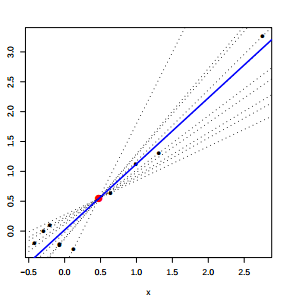
\includegraphics[scale=0.9]{img/rmc_atipico1.png}
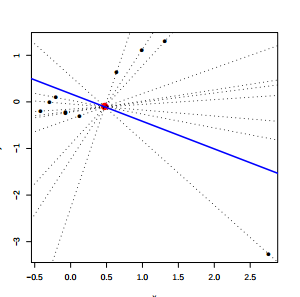
\includegraphics[scale=0.9]{img/rmc_atipico2.png}
\end{center}

\end{example}

\begin{example}[Sobre la distancia horizontal]

¿Y da igual lo atípico que sea un dato? La respuesta es que no. Si el dato es muy atípico en la variable respuesta ($Y$), pero es muy \textit{típico} en la variable regresora, la recta no se desvía tanto. Vamos a verlo y después explicamos la razón.

Esta es la recta, en la que hemos ignorado los 3 datos que parecen ``atípicos''.
\begin{center}
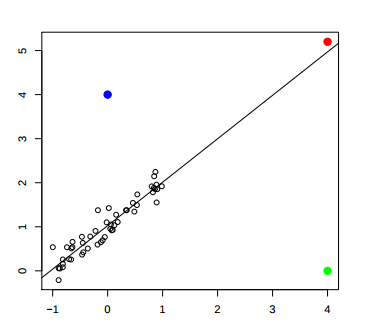
\includegraphics[scale=0.9]{img/sobredistanciahorizontal.png}
\end{center}

Ahora calculamos las rectas teniendo en cuenta sólo uno de los puntos.

\begin{center}
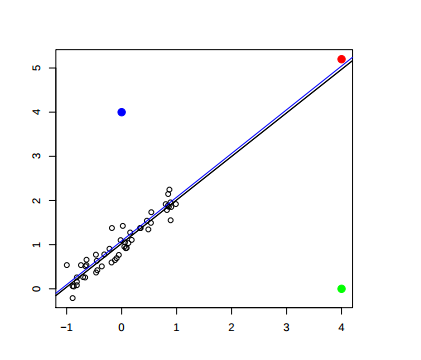
\includegraphics[scale=0.4]{img/sobredistanciahorizontal1.png}
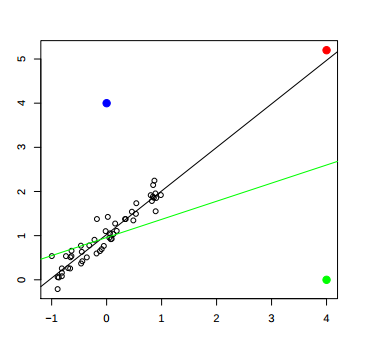
\includegraphics[scale=0.4]{img/sobredistanciahorizontal2.png}
\end{center}

Vemos que la recta azul no se desvía apenas de la original, mientras que la recta verde si se desvía un montón. ¿Esto a qué se debe? A que importa más la distancia horizontal de la media que la distancia vertical. Si vamos a la expresión de la recta de mínimos cuadrados como promedio de las pendientes \label{rmc::promediopendientes} vemos que hay un término $\frac{(x_i - \gor{x})}{S_{xx}}$ que hemos tomado como pesos para ponderar y en este caso, la distancia horizontal $(x_i - \gor{x})$ está multiplicando en el numerador.



\end{example}





\subsubsection{Introduciendo ``aleatoreidad'' para poder hacer IC}

Sea $\{ε_i\}$ siendo $ε_i \sim N(0,σ^2)$. Lo habitual es no saber cómo han sido generados los datos y es probable que no vayamos a conocer con exactitud absoluta la recta de mínimos cuadrados. Es por ello que suponemos el siguiente modelo para la variable respuesta:

\[
Y_i = β_1 x_i + β_0 + ε_i
\]


Tenemos que $\bar{y}_i \sim N$, ya que es una combinación lineal de variables normales \textbf{independientes} (como vimos en el Tema 1).


\begin{example}
Sea $σ=1, β_0 = 0$ y $β_1 = 1$.

Entonces el modelo es:

\[
Y_i = x_i + ε_i
\]

Fijamos $n=10$ y generamos las respuestas para $x_i = i$. Además, repetimos el experimento 6 veces y calculamos las rectas de mínimos cuadrados, obteniendo:

\begin{center}
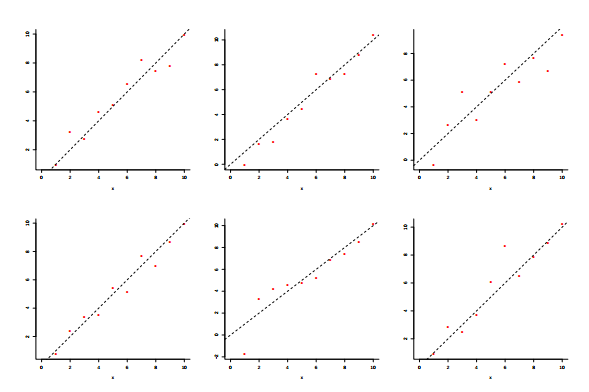
\includegraphics[scale=0.6]{img/6ejemplosRegresion.png}
\end{center}

Vemos que obviamente las rectas no son las mismas. Esto se debe al $ε_i$ introducido. ¿Cuáles son los valores que toman $β_1$ y $β_0$? Habiendo repetido el experimento 1000 veces, obtenemos los siguientes histogramas:

\begin{center}
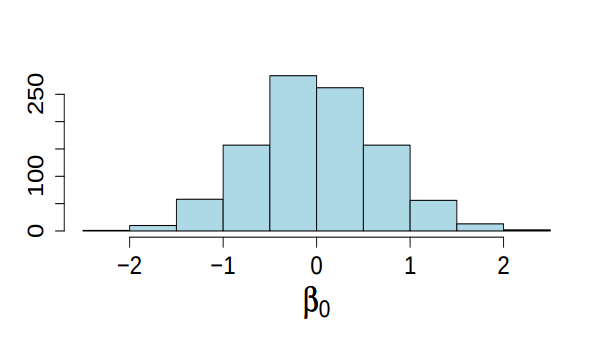
\includegraphics[scale=0.3]{img/1000vecesb0.png}
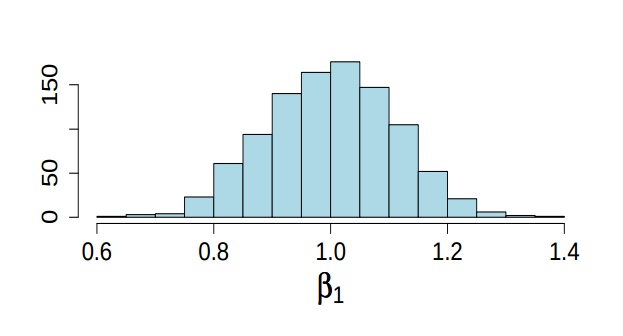
\includegraphics[scale=0.3]{img/1000vecesb1.png}
\end{center}

Vemos que no siempre es el mismo valor. Sabemos (por cómo hemos construido los datos) que $β_0 = 0$ y $β_1 = 1$, pero nuestra manera de calcularos (debido a $ε_i$) no siempre nos da el valor concreto.


\end{example}

El ejemplo anterior nos muestra que en realidad, estamos estimando $β_i$, aunque no nos guste y ahora tenemos que plantearnos ¿Cómo de buenos son nuestros estimadores? Tal vez son una mierda, o tal vez son insesgados.

Para ello, vemos que al haber añadido un error $\epsilon_i \sim N(0,σ^2)$, tenemos:

\[
Y_i = β_0 + β_1x + ε_i \implies Y_i \equiv N(β_0 + β_1X_i, σ^2)
\]


\subsubsection{Estimando $β_1$}

\begin{prop}
Nuestro estimador ``pendiente de la recta de mínimos cuadrados:'' $\hat{β_1}$  cumple

\[
\hat{β_1} \equiv N\left(β_1,\frac{σ^2}{S_{xx}} \right)
\]

\end{prop}

\begin{proof}
Él en clase lo ha hecho al revés. Muchos cálculos para llegar a la conclusión, pero aquí molamos más. En algún momento \textcolor{red}{revisará} alguien los apuntes y completará.

\begin{itemize}
	\item $\esp{\hat{β_1}} = β_1$
	\item $\var{\hat{β_1}} = ... = \displaystyle\frac{σ^2}{S_{xx}}$
\end{itemize}
\end{proof}

\subsubsection{Estimando $β_0$}

\begin{prop}
Nuestro estimador ``término independiente de la recta de mínimos cuadrados:'' $\hat{β_0}$  cumple

\[
\hat{β_0} = N\left(β_0 , σ^2 \left( \frac{1}{n} + \frac{\gor{x}^2}{S_{xx}}\right)  \right)
\]
\end{prop}

\begin{proof}
\begin{itemize}
	\item $\esp{\hat{β_0}} = β_0$
	\item
	$\var{\hat{β_0}} = \var{\gor{Y}} + \var{\hat{β_1}\gor{X}} - 2 \cov{\gor{Y},\hat{β_1}\gor{X}}$

 	\subitem Calculamos: $\cov{\gor{Y},\hat{β_1}\gor{X}}$ utilizando cosas del tema 1

 	\[
		\cov{\gor{Y},\hat{β_1}\gor{X}} = \cov{\frac{1'_n \gor{Y}}{n},α\gor{Y}} = \frac{1}{n}1'_nσ^2
 	\]
 	debido a que $α = 0$.

 	Ademas de ser incorrelados, son \textbf{independientes}. ¿Porqué? Porque conjuntamente son normales, es decir \[
 		\begin{pmatrix} \gor{Y} \\ \hat{β_1} \end{pmatrix} \equiv A\gor{Y} \equiv N_2
 	\]
\end{itemize}

\end{proof}


\textbf{Conclusiones:}
\begin{align*}
\gor{Y} &\text{ es independiente de } \hat{β_1}\\
\hat{β_1} &\equiv \left(β_1,\frac{σ^2}{S_{xx}}\right)\\
\hat{β_0} &\equiv \left(β_0,σ^2 \left( \frac{1}{n} + \frac{\gor{x}^2}{S_{xx}}\right)\right)
\end{align*}

¿Son estas las variables $\hat{β_1} $ y $\hat{β_0}$ normales una normal conjunta? Sí, \textbf{sí son una normal conjunta}. Una manera que tenemos de saber si es una normal conjunta es si son independientes, y en este caso no lo son.  Intuitivamente es fácil de ver. En una recta, si aumentamos la pendiente (y estamos en el primer cuadrante) entonces el término independiente disminuye.

Esta dependencia tiene que aparecer. Vamos a estudiar la covarianza entre los estimadores:

\[
\cov{β_1,β_0} = \cov{\gor{Y} - \hat{β_1}\gor{x}, \hat{β_0}} = ... = -\gor{x}\frac{σ^2}{S_{xx}}
\]


Pero sabemos que sí son una normal bidimensional porque toda combinación lineal de nuestros parámetros de la recta es una variable aleatoria (la variable regresora $\hat{Y}$) normal.


\subsubsection{IC y Contrastes para $β_1$}
\label{subsubsec:ICparaB1}

Recordamos que \[ \hat{β}_1 \equiv N\left(β_1,\frac{σ^2}{S_{xx}}\right)\]

Podemos normalizar y buscar una cantidad pivotal (como hacíamos en estadística I)

\[
\frac{\hat{β_1} - β_1}{\frac{σ}{\sqrt{S_{xx}}}} \equiv N\left(0,1\right)
\]

Pero aquí nos encontramos con que necesitamos $σ$, la varianza de los errores. Esta varianza a menudo no es conocida (porque no sabemos con exactitud cuál es la recta verdadera) y tenemos que estimarla.

Para estimarla, parece razonable usar \[ \hat{σ} = S_R =\frac{\sum_{i=1}^n e_i^2}{n-2}\]

\begin{expla}
Recordamos que para que estimar la varianza, utilizamos (por el lema de Fisher) $n-1$ de denominador para que el estimador sea insesgado. Esto sale de que en la demostración, hay una matriz de rango $n-1$ ya que existe una restricción.

Siguiendo este razonamiento, en este caso tenemos 2 restricciones\footnote{$\sum e_i = 0$ y $\sum e_ix_i = 0$}, por lo que si lo demostráramos rigurosamente, aparecería una matriz de rango $n-2$ y por eso es el denominador. De esta manera, conseguimos un estimador insesgado.

\end{expla}

Además, $S_R$ se denomina \concept{Varianza\IS residual}

\begin{prop}
Una pequeña generalización del lema de Fisher:
\[
\frac{(n-2)S_{R}^2}{σ^2} \equiv \chi_{n-2}^2
\]

Además, es independiente de $\hat{β_1}$

\end{prop}



\begin{proof}
Esta proposición es un caso particular de un teorema que veremos más adelante.
\end{proof}


Llamamos
\[ P_{R} = \frac{\hat{β_1}-β_1}{\frac{S_R}{\sqrt{S_{xx}}}}\]
\[ P_σ = \frac{\hat{β_1}-β_1}{\frac{σ}{\sqrt{S_{xx}}}}\]

Sabemos que $P_σ \sim N(0,1)$. Pero, al estimar ¿Se mantiene$P_R \sim N(0,1)$?

Al estimar $σ$,  $P_{R}$ no tiene porqué ser exactamente $N(0,1)$. Si $n\to ∞$, entonces $S_R = σ$ y entonces $P_σ = P_R = N(0,1)$, pero para otros valores de $n≠∞$...

Por ello, nos vemos en la necesidad de manipular $P_R$ algebraicamente a ver si conocemos qué distribución tiene (que debería ser algo cercano a una normal, ya que estamos estimando $σ$ con un estimador insesgado. Tal vez las colas de la distribución son menos pesadas y podríamos esperar que fuera una $t$)

\label{Cuentas:largas}

\[
\displaystyle\frac{\hat{β_1}-β_1}{\displaystyle\frac{S_R}{\sqrt{S_{xx}}}} = \displaystyle\frac{\hat{β_1}-β_1}{\displaystyle\frac{σ}{\sqrt{S_{xx}}}\frac{S_R}{σ}} = \left( \displaystyle\frac{\hat{β_1}-β_1}{\displaystyle\frac{σ}{\sqrt{S_{xx}}}} \right)\displaystyle\frac{1}{\displaystyle\frac{S_R}{σ}} = \displaystyle\frac{ \displaystyle\frac{\hat{β_1}-β_1}{\frac{σ}{\sqrt{S_{xx}}}} }{\displaystyle\frac{S_R}{σ}}
\]

En el numerador tenemos una $N(0,1)$ y en el denominador la raíz de una $\chi^2$ dividida por sus grados de libertad (por la proposición anterior). Esto es por definición una $t$ (T-Student) con los mismos grados de libertad que la $\chi^2$, es decir $n-2$. (\href{https://en.wikipedia.org/wiki/Student%27s\_t-distribution#Characterization}{Wikipedia})


\begin{prop}
Podemos calcular el intervalo de confianza  para la pendiente de la recta, utilizando la fórmula de intervalo de confianza

\[
IC_{1-α}(β_1) \equiv \left[ \hat{β_1} \mp t_{n-2,\frac{α}{2}}\frac{S_R}{\sqrt{S_{xx}}}\right] = \left[ \hat{β_1} \mp \mathcal{Z}\frac{σ}{\sqrt{S_{xx}}}\right] %\equiv \left[ \gor{Y} \mp \t_{n-1,\frac{α}{2}}\frac{S_R}{\sqrt{n}} \right]
\]
\end{prop}

\subsubsection{Contraste en R}

\label{example:R-output}
\begin{lstlisting}[style=mystyle]
# Ajusta el modelo
regresion = lm(Fracaso~Renta)
summary(regresion)

lm(formula = Fracaso ~ Renta)

Residuals:	Min		1Q			Median		3Q		Max
				-7.8717 -3.7421		0.5878	3.0368	11.5423
---
Coefficients:	Estimate Std.	Error 	t-value		Pr(>|t|)
(Intercept)		38.4944				3.6445	10.562		8.37e-10 ***
Renta 				-1.3467				0.2659	-5.065		5.14e-05 ***
---
Signif. codes: [...]
Residual standard error: 4.757 on 21 degrees of freedom
Multiple R-Squared: 0.5499,
Adjusted R-squared: 0.528
\end{lstlisting}


Aquí, la fila de \textit{intercept} es el término independiente y renta es la pendiente. Además, los p-valores son para el contraste $\hat{β_i} = 0$, dentro de la hipótesis $β_i \geq 0$. \footnote{Si queremos contrastar si es positivo, nos vamos al caso límite que lo separa y contrastamos eso}.

En este caso, el p-valor para $H_0: \hat{β_1}=$ es $5.14e-5$, con lo que no podemos rechazar la hipótesis.


\subsubsection{Predicciones}

Sea $(x_1,y_1),...,(x_n,y_n) \to y_i = β_0 + β_1x_i + ε_i$.

Dado una nueva observación $x_0$, tenemos 2 problemas para predecir:

\begin{itemize}
	\item \textbf{Inferencia sobre $m_0 \equiv \esp{y_0 | x_0} = β_0 + β_1x_0$}

	En este caso, $$\hat{m_0} = \hat{β_0} + \hat{β_1}x_0$$

	¿Cómo es este estimador?

	\[\esp{\hat{m_0}} = β_0 + β_1x_0 = m_0\]
	\[\var{\hat{m_0}} = ... = σ^2\left[\frac{1}{n} + \frac{(x_0-\bar{x})^2}{S_{xx}} \right] \]

	\subitem Intuitivamente, lo que significa el segundo sumando de la varianza es que ``cuanto más cerca esté $x_0$ de la media, mejor será la estimación''.

	\textbf{Conclusión:}

	\[
		\hat{m_0} \sim N\left( m_0, σ^2\left[\frac{1}{n} + \frac{(x_0-\bar{x})^2}{S_{xx}} \right]\right)
	\]



	\subitem \textbf{Intervalo de confianza} para $m_0$ utilizando la fórmula de intervalos de confianza:

	\[
IC_{1-α}(m_0) \equiv \left[ \hat{m_0} \pm t_{n-2,\frac{α}{2}}S_R\sqrt{\frac{1}{n} + \frac{(x - \gor{x})^2}{S_{xx}}}\right]
\]

	\item \textbf{Predecir $Y_0$} usamos de nuevo:

	\[
\hat{Y_0} = \hat{β_0} + \hat{β_1}x \to Y_0 - Y \equiv N\left( 0, σ^2\left( 1 + \frac{1}{n}+  \frac{(x-\gor{x})^2}{S_{xx}}\right) \right)
	\]

	Donde la varianza ha sido calculada:

	\[
	\var{Y_0 - \hat{Y_0}} = \underbrace{\var{Y_0}}_{σ^2} - \var{\hat{Y_0}} + \underbrace{2 \cov{Y_0,\hat{Y_0}}}_{ = 0 \text{ (indep.) }} = σ^2 + σ^2\left( \frac{1}{n}+  \frac{(x-\gor{x})^2}{S_{xx}} \right)
	\]


	Este es un problema más complicado, ya que tenemos que tener en cuenta el término de error $ε_i$ y es por esto que aparece el 1 en la varianza. Tenemos que tener en cuenta la incertidumbre.

	Estandarizando y cambiando $σ$ por $S$, tenemos:

	\[
	\frac{Y_0 - \hat{Y_0}}{S_r \sqrt{1 + \frac{1}{n} + \frac{(x-\gor{x})^2}{S_{xx}}}} \equiv t_{n-2}
	\]

	Ya que tenemos una normal estandarizada dividida por su .... que por definición, es una $t$ de student.

	Ahora, vamos a construir el \concept{intervalo de predicción} (cambia ligeramente la interpretación)

	\[
1 - α = P\left\{ -t_{n-2;\frac{α}{2}} < \frac{Y_0 - \hat{Y_0}}{...} < t_{n-2;\frac{α}{2}}    \right\} = P \left\{ Y_0 \in \left[ \hat{Y_0} \pm t_{n-2;\frac{α}{2}} S_R \sqrt{1+\frac{1}{n}+...} \right]  \right\}
	\]
\end{itemize}

Ahora vamos a hacer unos ejemplos numéricos.

\begin{example}Seguimos con el ejemplo de la renta.
\begin{problem}
\begin{center}
\begin{tabular}{c|c|c}
&media&desviación típica\\\hline
\% fracaso & 20.73 & 6.927\\
renta &13.19  & 3.814
\end{tabular}
La renta está expresada en miles de euros.
\end{center}


\ppart IC para $β_1$ de nivel $95\%$.
\ppart IC para \% de fracaso medio si la renta es de $14.000$ euros.


Es parte del enunciado la salida de ``R'' incluida en: \ref{example:R-output}

\solution
\spart

\[
IC_{1-α}(β_1) = \left[-1.3467 \mp t_{21;0.025} · (0.2659)\right]
\]

Donde el $-1.3467$ es el estimador $\gor{β_1}$ que obtenemos de la salida de $R$. Lo mismo el $0.2659$, que es el error típico.

\spart
\[ \gor{Y_0} = 38.49 - (1.3467) · \underbrace{14}_{x_0} = 19.64\]

Siendo este el estimador, vamos a construir el intervalo de confianza. \footnote{Podría ser que nos pidieran el intervalo de predicción, pero en ese caso estarían pidiendo el intervalo de ...... para predecir. Además, nos están dando un $x_0$ que para predicción no lo tenemos}

\[
IC_{1-α}(m_0) = \left[19.64 \mp (2.06)(4.757)\sqrt{\frac{1}{23}+\frac{(14-13.19)^2}{S_{xx}}}\right]
\]
Donde $S_{xx} = 320.06$ y podemos calcularlo despejando de:

\[
E.T.(\gor{β_1}) = \sqrt{\frac{S_R^2}{S_{xx}}} \to \sqrt{S_{xx}} = \frac{4.757}{0.2659} \to S_{xx} = 320.06
\]
Donde $E.T.(\gor{β_1})$ es el error típico dado por \textit{R}. En este caso es $0.2659$y $S_R^2 = 4.757^2$

También podríamos utililzar $S_x = \frac{S_{xx}}{n-1}$, sabiendo que $S_x^2 = \frac{n}{n-1}σ^2$. Sabemos que $S_x = 3.814$ por ser la renta la variable explicativa, es decir, las $x$ de nuestro modelo de regresión.

\[
\frac{n}{n-1}\left(3.814\right)^2 = \frac{S_{xx}}{n-1} \to S_{xx} = 21·\left(3.814^2·\frac{22}{21}\right) = 320.03
\]
\end{problem}


\end{example}


\obs Todos estos cálculos y todas estas fórmulas se basan en muchas hipótesis (como que la distribución del error sigue una distribución normal). Pero podría ser que esto no ocurriera y estuviéramos suponiendo un modelo falso. Para ello, en estadística existe el \concept{Diagnóstico del modelo}. Este diagnóstico, consiste en comprobar si las hipótesis del modelo son \textbf{aceptables} para los datos disponibles. ¡Ojo! Aceptable... Puede haber muchos modelos aceptables para un mismo conjunto de datos.

Este diagnóstico se suele basar en el análisis de los residuos del modelo.

\begin{example}
	Vamos a ver a ojo unos cuantos ejemplos. Vamos a utilizar que $\corr{e,\gor{y}} = 0$ bajo el modelo (como calculamos anteriormente)

\begin{center}
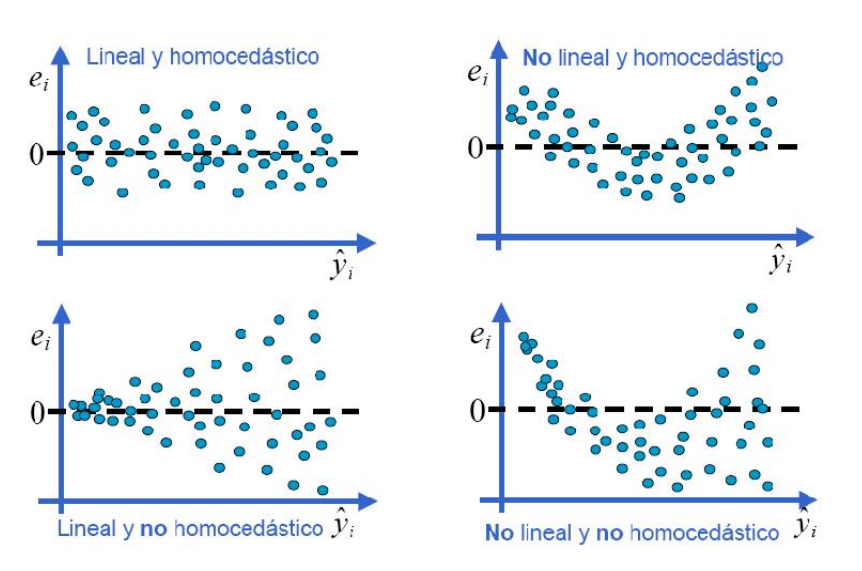
\includegraphics[scale=0.5]{img/diagmodelo.png}
\end{center}

De estos 4 gráficos, el bueno es el primero, ya que los demás no cumplen alguno.
\end{example}

\begin{example}
Vamos a ver otro ejemplo, donde arriba están los datos y abajo los residuos. Mirando sólo la fila de arriba podríamos saber si nuestro modelo para la regresión se cumple o sino.


\begin{center}
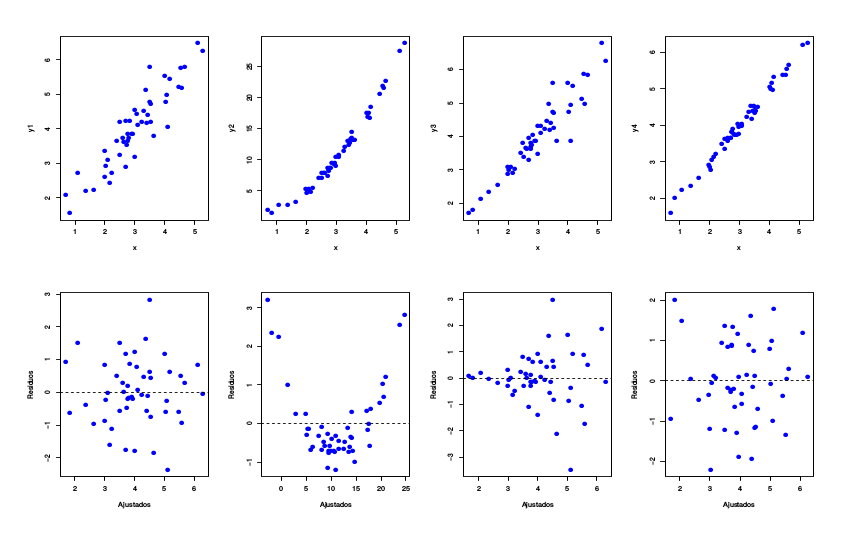
\includegraphics[scale=0.5]{img/diagmodelo_2.png}
\end{center}

Vemos que el primero y el último si tienen este modelo como aceptable, ya que en los residuos no hay ningún patrón (y se cumple que la correlación es 0).

En el segundo, podríamos suponer que es bueno, pero al diagnosticar el modelo mirando los residuos, vemos que no. El diagnóstico del modelo \textbf{magnifica los errores}.

En el cuarto, vemos más claro que es heterocedástico y que no se cumple el modelo supuesto.
\end{example}

En regresión múltiple veremos que no podemos ver los datos, ya que son demasiadas variables, pero sí podemos estudiar los residuos como acabamos de hacer en los ejemplos anteriores.


\subsection{Regresión lineal múltiple}

El ejemplo que vamos a estudiar en regresión múltiple es el consumo de gasolina en EEUU intentando predecirlo a partir de unas cuantas variables. Las variables regresoras son:

\begin{center}
\begin{tabular}{cccccccc}
State&Drivers&FuelC&Income&Miles&MPC&Pop&Tax\\\hline
AL&3559897&2382507&23471&94440&12737.00&3451586&18.0\\
AK&472211&235400&30064&13628&7639.16&457728&8.0\\
AZ&3550367&2428430&25578&55245&9411.55&3907526&18.0
\end{tabular}
\end{center}


Estos son los datos que obtenemos de $R$:

\begin{lstlisting}[style=mystyle]
reg <- lm(FuelC ~ Drivers+Income+Miles+MPC+Tax, data=fuel2001)
summary(reg)
Call:
lm(formula = FuelC ~ Drivers + Income + Miles + MPC + Tax, data = fuel2001)
Coefficients:
Estimate	Std.Error	t	value	Pr(>|t|)
(Intercept)	-4.844e+05	8.102e+05	-0.598	0.552903
Drivers	6.144e-01	2.229e-02	27.560	<	2e-16
Income	7.526e+00	1.611e+01	0.467	0.642587
Miles	5.813e+00	1.587e+00	3.664	0.000652
MPC	4.643e+01	3.488e+01	1.331	0.189820
Tax	-2.114e+04	1.298e+04	-1.629	0.110298
---
Residual standard error: 394100 on 45 degrees of freedom
Multiple R-squared: 0.9808, Adjusted R-squared: 0.9787
F-statistic: 459.5 on 5 and 45 DF, p-value: < 2.2e-16
\end{lstlisting}

\subsubsection{Notación}


\begin{itemize}
	\item $n$ es el número de observaciones, en este caso, el número de estados.
	\item $k$ es el número de atributos.
	\item $ε_i \sim N(0,σ^2)$
	\item $n\geq k+2$: esta hípótesis  es muy necesaria.\footnote{En la estadística, habría que rehacer el modelo para cuando $k>n$. ¿Y cuándo $k>n$? ¿Cuándo puede ocurrir esto? Cada vez más hay más información para cada individuo. En estudios genéticos por ejemplo, que hay millones de genes pero no se pueden hacer el estudio con millones de personas... \textbf{LA MALDICIÓN DE LA DIMENSIONALIDAD} que decimos en Introducción previa a los Fundamentos Básicos del Aprendizaje Automático.\\ Una posible solución al problema es un algoritmo que filtre los atributos que son importantes.}
\end{itemize}

Regresión simple es un caso particular de múltiple, tomando $k=1$.

\subsubsection{Modelo}

Tenemos una muestra de $n$ observaciones de las variables $Y$ y $X_1,…,X_k$. Para la observación $i$, tenemos el vector $(Y_i,x_{i1},x_{i2},…,x_{ik})$.

El modelo de regresión lineal múltiple supone que:
\[Y_i=β_0+β_1x_{i1}+…+β_kx_{ik}+ε_i,\ i=1,...,n\]

donde las variables de error $ε_i$ verifican:
\begin{enumerate}
\item $ε_i$ tiene media cero, para todo $i$.
\item Var($ε_i$) = $σ^2$, para todo $i$ (homocedasticidad).
\item Son variables independientes.
\item Tienen distribución normal.
\item $n ≥ k + 2$ (hay más observaciones que parámetros).
\item Las variables $X_i$ son linealmente independientes entre sí (no hay colinealidad).
\end{enumerate}

Las 4 primeras hipótesis se pueden reexpresar así: las observaciones de la muestra son independientes entre sí con
\[Y_i \equiv N(β_0 +β_1x_{i1} +...+β_kx_{ik},σ),\ i=1,...,n\]

En forma matricial:

\[
	\begin{pmatrix}
		Y_1\\
		Y_2\\
		\vdots \\
		Y_n
	\end{pmatrix}
	=
	\begin{pmatrix}
		1 & x_{11} & … & x_{1k} \\
		1 & x_{21} & … & x_{2k} \\
		\vdots & \vdots &  & \vdots \\
		1 & x_{n1} & … & x_{nk}
	\end{pmatrix}
	\begin{pmatrix}
		β_1\\
		β_2\\
		\vdots \\
		β_n
	\end{pmatrix}
	+
	\begin{pmatrix}
		ε_1\\
		ε_2\\
		\vdots \\
		ε_n
	\end{pmatrix}
\]


De forma más compacta, el modelo equivale a:
\[Y =Xβ+ε,\ ε \equiv N_n(0,σ^2I_n) \iff Y \equiv N_n(Xβ,σ^2I_n)\]

\begin{defn}[Matriz de diseño]
	La matriz $X$ se conoce como matriz de diseño
\end{defn}

\subsubsection{Estimación de los parámetros del modelo}

La pregunta que lógicamente se nos viene a la cabeza en este momento es: ¿Cómo estimar $β$ a partir de $Y$ y $X$?. Para ello nos serviremos de la interpretación geométrica del modelo:

Sea $\mathcal{V} ⊂ R^n$ el subespacio vectorial generado por las columnas de la matriz de diseño $X$ ($\dim(\mathcal{V}) = k + 1$).
\[μ∈\mathcal{V} \iff ∃β∈R^{k+1} : μ=Xβ\]
El modelo equivale a suponer $Y \equiv N_n(μ, σ^2I_n)$, donde $μ ∈ \mathcal{V}$.

\newpage
\begin{figure}[hbtp]
	\centering
	\inputtikz{proyecta_V}
\end{figure}

Con esto, parece razonable estimar $µ$ mediante la proyección ortogonal de $Y$ sobre $\mathcal{V}$ para obtener $\hat{Y} = X\hat{β}$. Equivalentemente: $\norm{Y-X\hat{β}}^2 \leq \norm{Y-Xβ}^2, ∀β\in ℝ^{k+1}$

\begin{defn}[Estimador mínimos cuadrados]

	Al $\hat{β}$ que minimiza
	\[\norm{Y - Xβ}^2 = \sum_{i=1}^n (Y_i - β_0 - β_1x_{i1} - … - β_kx_{ik})^2\]
	se le denomina estimador de mínimos cuadrados.
\end{defn}

Veamos qué podemos sacar de lo visto hasta ahora para averiguar quién es exactamente $\hat{β}$:

Para que $\hat{Y}$ sea la proyección de $Y$ sobre $\mathcal{V}$ es necesario y suficiente que se satisfagan las ecuaciones normales:

\begin{defn}[Ecuaciones normales]
	Tomando $e = Y - \hat{Y}$ como el vector residuo, las ecuaciones normales se satisfacen si:
	\[X'(Y - \hat{Y})=0 \iff X'e = 0\]
\end{defn}

Que se satisfagan estas ecuaciones es equivalente a decir que la resta $Y - \hat{Y}$ da un vector perpendicular a la base $\mathcal{V}$. Sustituyendo $\hat{Y} = X\hat{β}$:

\[X'(Y - X\hat{β}) = 0 \iff X'Y = X'X\hat{β}\]

Ya que las filas de $X'$ (las columnas de $X$) son independientes, sabemos que $X'X$ tiene rango completo y por tanto es invertible. Y llegamos a la expresión para nuestro estimador de mínimos cuadrados $\hat{β}$:
\begin{equation}
	\boxed{\hat{β} = (X'X)^{-1}X'Y}
\end{equation}


\begin{obs}
	En regresión simple se tiene que:
	\[
		X\equiv
		\begin{pmatrix}
			1 & x_1\\
			\vdots & \vdots \\
			1 & x_n
		\end{pmatrix}
		\text{ y que: }
		X'X =
		\begin{pmatrix}
			n & \sum x_i \\
			\sum x_i & \sum x_i^2
		\end{pmatrix}
	\]
\end{obs}

Con lo visto hasta el momento sabemos que $\hat{Y} = X\hat{β} = X(X'X)^{-1}X'Y$, es decir, que nuestra $\hat{Y}$ está expresada como producto de $Y$ por una matriz que llamaremos:

\begin{defn}[Hat matrix]
	\[H = X(X'X)^{-1}X'\]
	se conoce como hat matrix, puesto que da $Y$ gorro: $\hat{Y} = HY$.
\end{defn}

La hat matrix $H$ tiene las siguientes \textbf{propiedades}:
\begin{itemize}
	\item Es matriz de proyección ortogonal sobre $\mathcal{V}$.
	\item Es simétrica e idempotente.
	\item Tiene rango $k+1$ (la dimensión del espacio $\mathcal{V}$ sobre el que proyecta).
\end{itemize}

\begin{obs}
	Podemos servirnos de la hat matrix para expresar el vector de residuos:
	\[e = Y - \hat{Y} = Y - HY = (I - H)Y\]
	Donde $(I-H)$ es una matriz simétrica e idempotente con rango $rg(I-H)=~n-~(k~+~1)$, que proyecta sobre el espacio ortogonal $\mathcal{V}^\perp$.
\end{obs}

Para acabar esta sección enumeramos algunas propiedades de los parámetros:
\begin{itemize}
\item $\hat{β}$ es el estimador de máxima verosimilitud (EMV) de $β$:
\[L(β,σ)= \left(\frac{1}{\sqrt{2π}σ}\right)^n exp\left\{-\frac{1}{2σ^2} \norm{Y−Xβ}^2 \right\}.\]

\item El EMV de $σ^2$ es:
\[\hat{σ}^2 = \frac{\norm{Y−Xβ}^2}{n} = \frac{\norm{e}^2}{n} = \frac{\sum_{i=1}^n e_i^2}{n}\]

\item El vector $\hat{β}$ tiene distribución $N_{k+1}(β, σ^2(X′X)^{−1})$ (en la siguiente sección se demuestra).
\end{itemize}

\subsubsection{Estudio de la varianza residual}
Un estimador insesgado de $σ^2$ es la varianza residual $S_R^2$ , es decir, la suma de los residuos al cuadrado, corregida por los grados de libertad apropiados (en este caso $n-\dim{(\mathcal{V})}$):
\[S_R^2 = \frac{\sum e_i^2}{n-(k+1)} = \frac{\norm{e}^2}{n-k-1} = \frac{\norm{Y - \hat{Y}}^2}{n-k-1}\]

Si nos fijamos en que:
\[\norm{Y - \hat{Y}}^2 = Y'(I-H)(I-H)Y = Y'(I-H)Y\]

y sabiendo que la matriz $I-H$ es simétrica e idempotente, si recordamos la proposición \ref{prop:tema1_pepino} y demostramos $μ(I-H)μ'=0$, podemos determinar que la distribución de $S_R^2$:

Dado que $μ∈\mathcal{V}$ y sabiendo que $μ=XB$:
\[(I-H)μ = (I-H)XB = 0\]
Ya que el vector $(I-H)$ proyecta sobre $\mathcal{V}^\perp$.

Así llegamos a que:
\[\frac{\norm{Y-\hat{Y}}^2}{σ^2} = \frac{Y'(I-H)Y}{σ^2}=\]
\begin{equation}
	\boxed{\frac{(n-k-1)S_R^2}{σ^2} \equiv χ_{n-k-1}^2}
\end{equation}


Además si tomamos esperanzas en ambos lados de la igualdad obtenemos:
\[\frac{(n-k-1)·\mathbb{E}(S_R^2)}{σ^2} = n-k-1\]
\begin{equation}
	\boxed{\mathbb{E}(S_R^2) = σ^2}
\end{equation}

Lo siguiente que haremos es mirar si $\hat{β}$ y $S_R^2$ \textbf{son independientes}. Esto es cierto dado que se cumple que $(X'X)^{-1}X' · (I-H)=0$:
\[(X'X)^{-1}X' · (I-H) = (X'X)^{-1}X' - (X'X)^{-1}X' · X(X'X)^{-1}X' =0\]

\begin{obs}
	El lema de Fisher \ref{lemma:fisher} no es más que el resultado de aplicar los resultados vistos en esta sección al caso particular del modelo:
	\[y_i = β_0 + ε_i \iff X=\begin{pmatrix}1\\ \vdots \\ 1\end{pmatrix}\]
	En este caso tenemos que $\dim{(V)}=1$
\end{obs}


\subsubsection{Distribución de $\hat{β}$ y contrastes de hipótesis individuales sobre los coeficientes $\hat{β}_i$}
\[\esp{\hat{β}} = (X'X)^{-1}X' \underbrace{Xβ}_{\esp{Y}} = β\]
\[\var{\hat{β}} = σ^2I_n · (X'X)^{-1}X' · X(X'X)^{-1} = σ^2(X'X)^{-1}\]

Como $\hat{β}$ es una combinación lineal de $Y$ (que sigue una distribución normal):

\[
\hat{β} \equiv N_{k+1}\left(β,σ^2(X'X)^{-1}\right)
\]

Y la regresión simple, es un caso particular de esta fórmula.

\textbf{Notação}: $q_{ij}\equiv$ entrada $i,j$ de la matriz $(X'X)^{-1}$

\paragraph{Consecuencias:}

\begin{itemize}
	\item ¿Cuál es la distribución marginal de $\hat{β_j}$ a partir de la que hemos visto de la conjunta? Como vimos en el tema 1, es también una normal, con el correspondiente valor del vector $β$ como media y el elemento $j,j$ de la diagonal.
	\[ \hat{β}_j \equiv N\left(β_j, σ^2q_{jj}\right)\]

	Ahora, podemos estandarizar:

	\[
	\frac{\hat{β_j}-β_j}{σ\sqrt{q_{jj}}} \equiv N(0,1)
	\]

	Y utilizando que $S_R$ es independiente de $σ$ y la definición de $t-$student tenemos:

	\[
	\frac{\hat{β_j}-β_j}{S_R\sqrt{q_{jj}}} \equiv t_{n-k-1}
	\]

	¿Cuál es el intervalo de confianza?

	\[
		IC_{1-α}(β_j) \equiv \left[\hat{β_j}\mp t_{n-k-1;\frac{α}{2}}\underbrace{S_R\sqrt{q_{jj}}}_{\text{Error típico de }β_j} \right]
	\]

	Y, como en regresión simple, estudiamos $H_0 : β_j = 0$:
	\[
		R = \left\{ \frac{\abs{\hat{β}_j}}{S_R\sqrt{q_{jj}}} > t_{n-k-1;\frac{α}{2}} \right\}
	\]
\end{itemize}

En las traspas encontramos una salida de regresión múltiple de $R$. La columna \textit{estimate} es el vector $\hat{β}$, el p-valor es del contraste $H_0 : β_j = 0$.


\subsubsection{Combinaciones lineales de los coeficientes} Vamos a querer constrastar cosas del estilo ¿las 2 variables influyen igual?

Para ello, transformamos eso en $H_0: β_1 = β_2 \to H_0 : β_1 - β_2 = 0$, entonces tenemos una combinación lineal $a∈ℝ^{k+1}$, tal que $H_0:a'\hat{β} = 0$

Para poder hacer esto, lo primero ha sido estimar $\hat{β}$ y lo siguiente será saber su distribución.

\[a'\hat{β} = N\left(a'β,\underbrace{σ^2a'(X'X)^{-1}a}_{\left(E.T.(a'\hat{β})\right)^2}\right) \to \frac{a'\hat{β} - a'β}{S_R\sqrt{a'(X'X)^{-1}a}} \equiv t_{n-k-1}\]

Y con esto, ya podemos construir el intervalo de confianza para una combinación lineal de los parámetros:

\[
IC_{1-α}(a'β) = \left[ a'\hat{β} \mp t_{n-k-1;\frac{α}{2}}E.T.(a'\hat{β}) \right]
\]

La región de rechazo correspondiente es:

\[
R = \left\{ \frac{a'\hat{β}}{S_R\sqrt{σ^2a'(X'X)^{-1}a}} >  t_{n-k-1;\frac{α}{2}} \right\} = \left\{ \frac{a'\hat{β}}{E.T.(\hat{β})} >  t_{n-k-1;\frac{α}{2}} \right\}
\]

\paragraph{Ejercicio:} ¿Y si queremos hacer un contraste unilateral $a'β > 0$?

\subsubsection{Inferencia sobre subconjuntos de coeficientes}

Todos los contrastes hechos hasta ahora son muy fáciles porque se basan en una única normal. Nuestros contrastes han sido del tipo $β_i = 0$. En esta sección vamos a estudiar contrastes del tipo $H_0: β_1 = 0, β_3 = 0$.

La primera aproximación puede ser calcular la región de confianza de $β_1$ y la de $β_3$ y tomar la intersección. Es decir:

\begin{center}
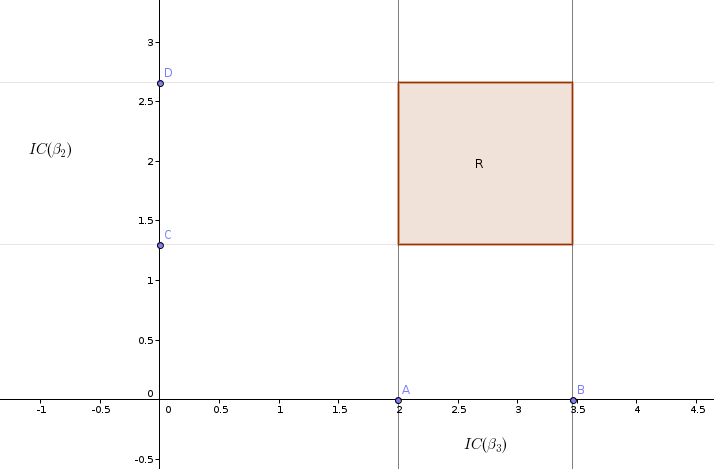
\includegraphics[scale=0.5]{img/confianzamultivariantemal.png}
\end{center}

 Pero al no ser independientes, no estamos teniendo en cuanto las correlaciones, la información que me da saber $β_1$ para saber $β_3$.

\begin{center}
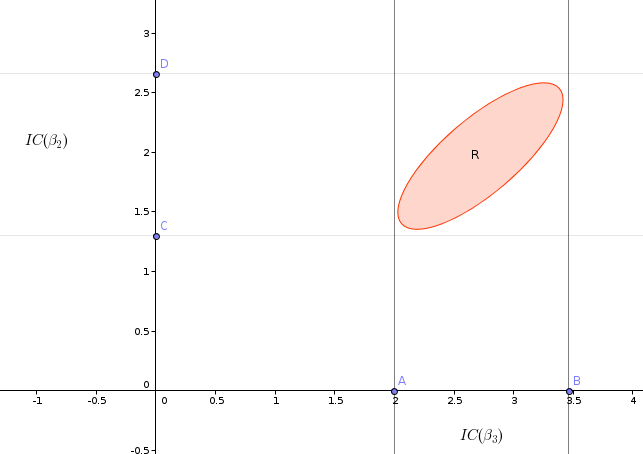
\includegraphics[scale=0.5]{img/confianzamultivariantebien.png}
\end{center}

\paragraph{Vamos a ello formalmente:}
\newcommand{\bpp}{β_{(p)}}
\newcommand{\hbpp}{\hat{β}_{(p)}}
\newcommand{\fpnk}{F_{p,n-k-1}}
Sea $β_{(p)}$ un conjunto de coeficientes de $β$. Sea $\hbpp$ el correspondiente subconjunto de estimadores.

Sea $Q_q$ la submatriz de $(X'X)^{-1}$ cuyas filas y columnas corresponden a las coordenadas del vector $\bpp$.

\[\hbpp \equiv N_p \left( \bpp, σ^2Q_p \right)\]

Si este es nuestro estimador, vamos a estandarizarlo (utilizando propiedades del tema 1).

\[
\frac{(\hbpp - \bpp)'Q_p^{-1}(\hbpp - \bpp)}{σ^2}\equiv \chi^2_p
\]

Tenemos el problema de que no conocemos $σ$ y tenemos que estimarlo. Para ello, vamos a seguir un proceso parecido a \ref{Cuentas:largas}. Para ello necesitamos:

\begin{defn}[Distribución $F_{n,m}$]

\[
F_{n,m} \equiv \frac{\chi^2_m / m}{\chi^2_n / n}
\]

Es muy habitual que aparezca la $F$ al comparar varianzas.
\end{defn}

Sabiendo lo que es una $F$, vamos a estudiar qué ocurre al cambiar $σ$ por $S_R$

\[
\frac{(\hbpp - \bpp)'Q_p^{-1}(\hbpp - \bpp)}{S_R^2} = \frac{\frac{(\hbpp - \bpp)'Q_p^{-1}(\hbpp - \bpp)}{σ^2}}{\frac{S_R^2}{σ^2}}
\]

En el numerador tenemos una $\chi^2_p$, pero nos faltaría dividir por los grados de libertad para tener una $F$, entonces:

\[
\frac{\frac{(\hbpp - \bpp)'Q_p^{-1}(\hbpp - \bpp)}{pσ^2}}{\frac{S_R^2}{σ^2}} = \frac{\chi^2_p/p}{\chi^2_{n-k-1}/n-k-1} \equiv F_{p,n-k-1}
\]

\paragraph{Conclusión}

%TODO: esto está bien seguro
\[
\frac{(\hbpp - \bpp)'Q_p^{-1}(\hbpp - \bpp)}{pS_R^2} \equiv F_{p,n-k-1}
\]
\[
1-α = P\left( (\hbpp - \bpp)'\left(S_R^2Q_p\right)^{-1}(\hbpp - \bpp) \leq p F_{p,n-k-1}\right)
\]

Esto nos da un elipsoide de confianza, es decir, sabemos que caerá en la región del elipsoide con probabilidad $1-α$:

\begin{figure}[hbtp]
	\centering
	\inputtikz{elipsoide_confianza}
\end{figure}

\begin{example}
Vamos a querer contrastar si son iguales los coeficientes $β_2,β_3$ las variables ``Income'' y ``Miles''. La hipótesis es: $H_0 : β_2=β_3$ a nivel $α=0.05$

Aquí damos los datos necesarios para completar (en la realidad, los obtendremos de $R$:
\[
S_R^2Q_{(2)} = \begin{pmatrix} 259.45&7.89\\7.89&2.52 \end{pmatrix}
\]

Vamos a proceder al contraste. Construimos el estadístico para construir la región de rechazo:

\[
t = \frac{|\hat{β_2} - \hat{β_3}|}{E.T.(\hat{β_2}-\hat{β_3})} = \frac{1.725}{15.687} \not \ge t_{45;0.025}
\]

Por tanto no podemos rechazar la hipótesis nula de que $β_2=β_3$.

El error típico se ha calculado es:
\[\sqrt{\var{\hat{β_2}-\hat{β_3}}} = \sqrt{(1,-1) S_R^2Q_p (1,-1)} = 15.687\]
Y los 45 grados de libertad los obtenemos de $R$.

\end{example}

\subsubsection{Predicción}

\paragraph{Confianza de $Y_0 | X_0$}
\[
m_0 = E(Y_0 | X_0) = β'X_o \to \hat{m_0} \equiv N\left( β'X_0 , σ^2X'_0(X'X)^{-1}X_0 \right)
\]
Ahora ya podemos calcular el intervalo de confianza para $Y_0$ dado un vector $X_0$.

\[
\left[ \hat{Y_0} \mp t_{n-k-1;\frac{α}{2}} S_R\sqrt{X_0'(X'X)^{-1}X_0} \right]
\]


\paragraph{Predicción de $Y_0$}

\[
\left[ \hat{Y_0} \mp t_{n-k-1;\frac{α}{2}} S_R\sqrt{1+X_0'(X'X)^{-1}X_0} \right]
\]

\section{Análisis de la varianza (ANOVA)}

Las variabilidades se miden mediante la suma de cosas al cuadrado. Vamos a definir 3 sumas de cuadrados:

\begin{defn}[Suma de cuadrados\IS total]
Medimos la variabilidad total con:
\[SCT = \sum_{i=1}^n (Y_i - \gor{Y})^2\]

Esta suma de cuadrados, mide la variabilidad ``real'' de los datos. Aquí no hay ningún modelo.
\end{defn}

\begin{defn}[Suma de cuadrados\IS de la regresión]
Medimos la variabilidad explicada por el modelo con:

\[SCR = \sum_{i=1}^n (\hat{Y_i} - \gor{Y})^2\]

Esta suma de cuadrados, mide la variabilidad según el modelo. En caso de $SCT = SCR$, tendríamos que el modelo es perfecto.
\end{defn}



\begin{defn}[Suma de cuadrados\IS total]
Medimos la variabilidad no explicada.

\[SCE = \sum_{i=1}^n (Y_i - \hat{Y_i})^2\]

\end{defn}


Intuitivamente, si el modelo estuviera bien construido sería razonable esperar que $SCT = SCR + SCE$.
Vamos a complicarnos la vida y utilizar la interpretación geométrica para ver que esa relación es cierta:


\paragraph{SCT vectorialmente}

\[
SCT = ||Y - \gor{Y}1_n||^2
\]

Vamos a ver una manera complicada de entender la media muestral: Proyección de un vector al espacio de proyección de los vectores con las mismas coordenadas. ¿Esto a qué viene?
\[
\gor{Y}1_n = \frac{1}{n}1_n1'_nY = MY
\]
Siendo \[M = \begin{pmatrix}\frac{1}{n} & ... & \frac{1}{n} \\ \vdots & \ddots & \vdots \\ \frac{1}{n} & ... & \frac{1}{n}\end{pmatrix}\]

Entonces, podemos construir:

\[
SCT = ||Y - \gor{Y}1_n||^2  = || Y-MY||^2 = ||(I-M) Y||^2 = Y'(I-M)Y
\]

\paragraph{SCR vectorialmente}
\[
SCR = || HY-MY||^2 = Y'(H-M)'(H-M)Y
\]

Necesitamos ver que $H-M$ es una matriz simétrica e idempotente. Recordamos que $H$ es la matriz de proyección sobre $\mathcal{V}$.

\[
(H-M)(H-M) = HH - MH - HM + MM \overset{(1)}{=} H - M
\]
$(1)$ sabemos que $HH = H$ y $MM=M$ porque ambas son idempotentes. Pero para tener una $M$ restando, necesitaríamos $MH = HM = M$.

Geométricamente, es fácil ver que $HM=M$. Esto se debe a que $M$ es la proyección sobre un espacio vectorial más pequeño e incluido en $H$, entonces al haber proyectado con $M$, volver a proyectar con $H$ no nos cambia nada.

Por otro lado, $MH = M$. En este caso, primero proyectamos en el subespacio grande, pero como acabamos proyetando sobre el pequeño.

\paragraph{Ejercicio: } Demostrar algebraicamente $MH=HM=M$.

\paragraph{SCE vectorialmente}
\[SCE = ||HY-H||^2 = Y'(I-H)Y\]

\begin{prop}[Relación de las sumas de cuadrados]
\[SCT = SCR + SCE\]
\end{prop}

\begin{proof}
\[SCT = Y'(I-M)Y = Y'(H-M+I-H)Y = Y'(H-M)Y + Y'(I-H)Y = SCR + SCE\]
\end{proof}

\begin{figure}[hbtp]
	\centering
	\inputtikz{relacion_SCE_SCT_SCR}
	\caption{Representación de los vectores $SCE,SCT,SCR$ sobre el espacio vectorial $\mathcal{V}$.}
\end{figure}

\subsubsection{Contraste de la regresión}
Queremos contrastar $H_0 : β_1 = ... = β_n = 0$.

La idea intuitiva es que si $SCR$ es muy pequeño, tenemos poca variabilidad explicada sería razonable que aceptáramos la hipótesis nula de que las variables regresoras no influyen mucho.

Por el contrario, si $SCR$ es muy \textbf{grande}, tenemos mucha variabilidad explicada, por lo que la hipóteis nula no es muy razonable y deberíamos \textbf{rechazar}. Por el contrario, si $SCR$ es \textbf{pequeña} aceptamos $H_0$.


Para ello, es imprescindible definir ``grande'' y ``pequeño''. Deberían tener las mismas unidades. No puede ser que por cambiar de unidades afecte a la validez de la hipótesis. Además, necesitamos saber la distribución de $SCR$ bajo la hipótesis nula. 

\begin{prop}[Distribución SCR en $H_0:∀i\;β_i=0$]

\[
\frac{SCR}{σ^2} \equiv \chi^2_{k}
\]
\end{prop}
\begin{proof}
Tenemos $SCR = Y'(H-M)Y$, una forma cuadrática, teniendo $H-M$ simétrica e idempotente (por construcción).

Ahora, para poder aplicar la proposición del tema 1, necesitamos $µ'(H-M)µ = 0$.

Sabemos que $µ$, bajo $H_0$ tiene todas sus coordenadas iguales, con lo que está en el subespacio $1_n$, por lo que las proyecciones sobre $V$ y sobre $1_n$ de $µ$ serán $µ$. Esto quiere decir que:
\[ Hµ = µ \;\;\; Mµ = µ \to (H-M)µ=0\]


Por otro lado, los $k$ grados de libertad:
\[
gl = \rg(H-M) = \tr(H-M) = \tr(H) - \tr(M) = (k+1)-1 = k
\]

Esto se debe a que la traza de una matriz de proyección es la dimensión del espacio en el que proyectamos.

\end{proof}

As usual, como no conocemos $σ^2$, en la práctica utilizamos:
\begin{prop}
\[
\frac{\displaystyle\frac{SCR}{kS_R^2}}{\displaystyle\frac{SCE}{n-k-1}} = \frac{\chi^2_k}{\chi^2_{n-k-1}}\sim F_{k;n-k-1}
\]
\end{prop}
\begin{proof}
Para ello necesitamos que $SCR$ y $SCE$ sean independientes. Son normas al cuadrado de vectores ortogonales. Estadísticamente, la ortogonalidad de vectores normales se traduce en independencia. 

Para ello, vamos a ver que el producto de las matrices es 0 (utilizando la propiedad \ref{prop:tema1_pepino})

\[
(H-M)(I-H) = H-H-M+\underbrace{MH}_{M} = 0
\]
Sabemos que $MH=M$ por que, por un lado es proyectar en $V$ después de haber proyectado en un subespacio de $V$ ($1_n$) y en el otro, tenemos la proyección directamente sobre $1_n$.

\end{proof}

\subsubsection{Tabla anova}
Para este caso, vamos a construir la tabla \concept{ANOVA} (análisis de la varianza)

Este es el ejemplo de una tabla ANOVA simple:
\begin{center}
\begin{tabular}{c|ccccc}
Fuente de variación & SC & gl & CM & F & p-valor\\\hline 
Explicada & SCR & k & $\frac{SCR}{k}$ & $\displaystyle\frac{SCR/k}{SCE/(n-k-1)}$ & ...\\
No explicada & SCE & n-k-1 & $\frac{SCE}{n-k-1}$ & ... & ...\\\hline
total & & & & 
\end{tabular}
\end{center}

\subsubsection{Coeficiente de determinación}
\begin{defn}[Coeficiente\IS de determinación]
Es una medida de la bondad del ajuste en el modelo de regresión múltiple \[R^2 = \frac{SCR}{SCT}\]
\end{defn}

\paragraph{Propiedades:}
\begin{itemize}
	\item $R^2≤1$ (ya que un cateto siempre es menor o igual que la hipotenusa)
	\item Vamos a ver los casos extremos.
	\subitem $R^2 = 1$ quiere decir que existe una relación lineal exacta debido a que \[R^2 = 1\implies SCR = SCT \implies SCE=0 \implies ∀i\;e_i=0\]

	De hecho, podemos interpretar $R^2$ como un coeficiente de correlación múltiple entre las $k$ variables $X$ y la $Y$.
	\subitem $R^2 = 0$ quiere decir que no existe una relación lineal debido a que \[R^2 = 0 \implies Σ(\hat{Y_i} - \gor{Y})^2 = 0 \implies \hat{Y_i}=\gor{Y} \implies \text{ ninguna X aporta información para calcular Y}\]
	\item Se verifica que el estadístico $\displaystyle F = \frac{R^2}{1-R^2} \frac{n-k-1}{k}$
	\begin{proof}
		Esta identidad se obtiene inmediatamente utilizando la definición de $R^2$. Se deja como ejercicio para quien quiera escribirse la cuenta.
	\end{proof}
\end{itemize}

Este coeficiente es útil en el contraste que estudiábamos anteriormente $H_0: ∀i\;β_i = 0$. En este contraste, es equivalente para rechazar o aceptar \begin{itemize}
	\item $SCR$ es ``grande''.
	\item $F$ es ``grande''.
	\item $R^2$ se aproxima a 1.
\end{itemize}


El coeficiente de determinación para comparar distintos modelos de regresión entre sí tiene el siguiente inconveniente:
Siempre que se añade una nueva variable regresora al modelo, $R^2$ aumenta, aunque el efecto de la variable regresora sobre la respuesta no sea significativo. ¿Porqué aumenta $R^2$? Porque la dimensión de $V$ aumenta provocando que disminuya $SCE$ (por algo que me he perdido) y al disminuir $SCR$, aumenta $SCR$ (porque su suma es constante) y aumenta $R^2$.

Por ello, definimos:


\begin{defn}[Coeficiente de determinación ajustado]
\[\gor{R}^2 = 1 - \frac{SCE/(n-k-1)}{SCT/(n-1)}\]
Esta nueva definición penaliza un aumento de las variables utilizadas. De esta manera, al aumentar $K$, sabemos que $R^2$ aumenta pero $\gor{R}^2$ puede aumentar o no. Depende de si la ganancia de información es mayor que la penalización de añadir más variables.
\end{defn}

Vamos a ver un ejemplo realmente ilustrativo.
\begin{example}

Vamos a utilizar el modelo de regresión múltiple para ajustar el grado del polinomio.

El proceso a seguir podría ser: voy calculando $R^2$ para todos los grados que vaya teniendo hasta que tenga $R^2 = 1$, que hace que podamos explicar toda la varianza con estos datos. 


Al aumentar el grado, obtenemos polinomios cada vez mejores (para estos datos).

\begin{center}
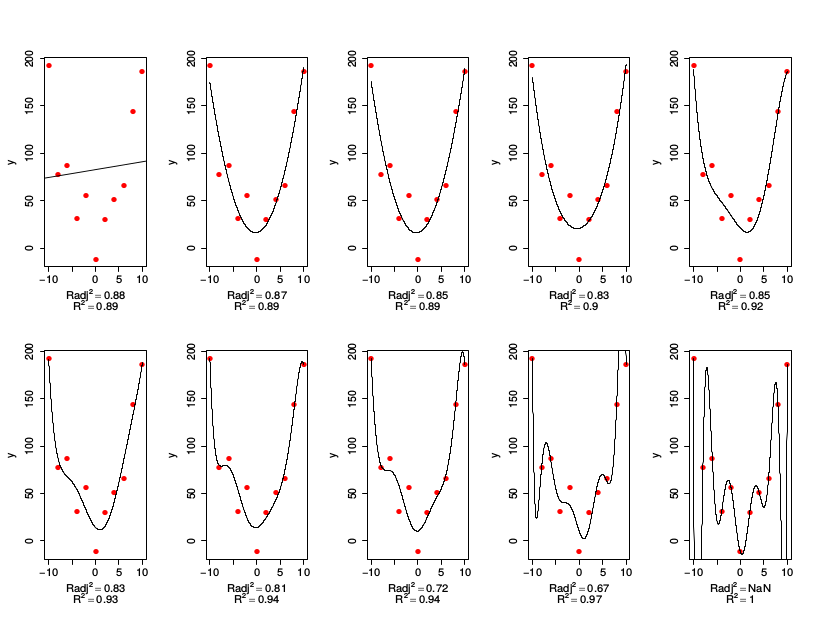
\includegraphics[scale=0.45]{img/RvsRAdj.png}
\end{center}

Si tomáramos una nueva muestra de datos, el modelo que tiene $R^2=1$ sería una mierda muy probablemente. En este caso, sería una bazofia absoluta ya que los datos han sido generados parabólicamente. Es por ello que el modelo con mayor $\gor{R}^2$ es el segundo.

\end{example}


\begin{example}

Si un modelo es demasiado simple, tendremos muy poca varianza pero mucho sesgo. Por el otro lado, si el modelo es demasiado complejo, tenemos mucha varianza pero muy poco sesgo. Vamos a verlo con un ejemplo:

\begin{center}
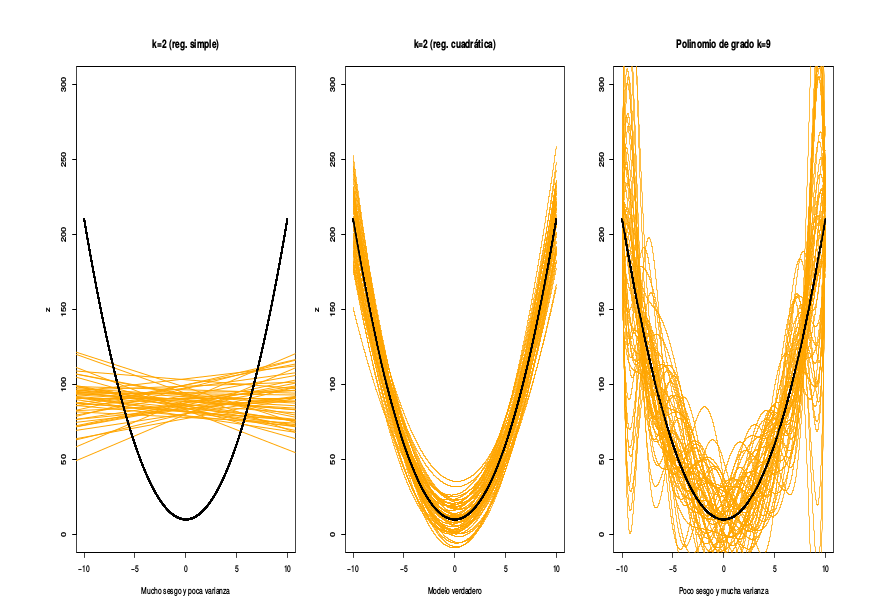
\includegraphics[scale=0.45]{img/ModeloSimpleVsModeloComplejo.png}
\end{center}

En este ejemplo corroboramos lo dicho.
	
\end{example}

\subsection{Contrastes de hipótesis lineales}
\subsection{Modelo unifactorial}




\appendix
\chapter{Ejercicios}
% -*- root: ../EstadisticaII.tex -*-

%%%%%%%%%%%%%%%%%%%%%%%%%%%%%%%%%%%%%%%%%%%%%%%%%%%%%%%%%%%%%%%%%%%%%%%%%%%%%%%%%%%%%%%%%%%%%%%
%%% 																						%%%
%%% 								HOJA 	1												%%%
%%% 																						%%%
%%%%%%%%%%%%%%%%%%%%%%%%%%%%%%%%%%%%%%%%%%%%%%%%%%%%%%%%%%%%%%%%%%%%%%%%%%%%%%%%%%%%%%%%%%%%%%%

\section{Hoja 1}

\begin{problem}[1]
Sea $\vec{Y} = (Y_1,Y_2,Y_3)' ≡ N_3(\vec{µ},Σ)$, donde \[\vec{µ} = (0,0,0)'\;
Σ =\begin{pmatrix}
1&0&0\\
0&2&−1\\
0&−1&2
\end{pmatrix}
\]


\ppart  Calcula la distribución del vector $\vec{X} = (X_1,X_2)$, donde $X_1 = Y_1 + Y_3$ y $X_2 = Y_2 + Y_3$.
\ppart ¿Existe alguna combinación lineal de las variables aleatorias $Y_i$ que sea independiente de $X_1$?

\solution
\doneby{Dejuan}


\spart 
\[
\begin{pmatrix}X_1 \\ X_2 \end{pmatrix} = \begin{pmatrix} Y_1 + Y_3 \\ Y_2 + Y_3 \end{pmatrix} = \begin{pmatrix} 1&0&1\\0&1&1 \end{pmatrix} \begin{pmatrix} Y_1\\Y_2\\Y_3 \end{pmatrix} 
\]

Ya tenemos la matriz $A$ que cumple $\vec{X} = A \vec{Y}$. Utilizando las propiedades de esperanza y varianza (\ref{propiedades:esperanzaYvarianza}):

\[\esp{\vec{X}} = \esp{A\vec{Y}} = A\esp{\vec{Y}} = \begin{pmatrix} 1&0&1\\0&1&1 \end{pmatrix} \begin{pmatrix} 0 \\0\\0\end{pmatrix} = \begin{pmatrix} 0 \\0\\0\end{pmatrix}\]

\[\var{\vec{X}} = \esp{A\vec{Y}} = AΣA' = \begin{pmatrix} 1&0&1\\0&1&1 \end{pmatrix} \begin{pmatrix}
1&0&0\\
0&2&−1\\
0&−1&2
\end{pmatrix} \begin{pmatrix} 1&0\\0&1\\1&1 \end{pmatrix} = \begin{pmatrix}3&1\\1&2\end{pmatrix}\]

\paragraph{Conclusión:}

\[\begin{pmatrix}X_1 \\ X_2 \end{pmatrix} \equiv N_1\left( \begin{pmatrix}0\\0 \end{pmatrix},\begin{pmatrix}3&1\\1&2\end{pmatrix} \right)\]


\spart Llamos $Z = a_1 Y_1 + a_2Y_2+a_3Y_3$.


Estas variables serán independientes si se distribuyen conjuntamente como una normal multidimensional y si $\cov{Z,X_1} = 0$.


Vamos a ver la covarianza. Utilizando la propiedad definida en \ref{propiedad:CovCombinacionLineal}, tenemos que

\[
\cov{a_1Y_1 + a_2Y_2 + a_3Y_3 , X_1} = \cov{A\vec{Y},B\vec{Y}}
\]

Siendo $A = (a_1,a_2,a_3)$ y $B=(1,0,1)$

Entonces \[\cov{A\vec{Y},B{\vec{Y}}} = (a_1,a_2,a_3) \begin{pmatrix} 1&0&0\\0&2&-1\\0&-1&2\end{pmatrix} \begin{pmatrix} 1\\0\\1 \end{pmatrix}\]

Operando obtenemos $\cov{A\vec{Y},X_1} = a_1 - a_2 + 2a_3$.



Ahora sólo hace falta ver que se distribuyen conjuntamente como una normal bivariante. Esto lo tenemos asegurado, pues ``\textit{El vector se distribuye normalmente porque lo podemos escribir en la forma AY, para una matriz A.}''\footnote{Cito textualmente de un correo envíado por José Ramón, profesor de la asignatura}
\end{problem}


\begin{problem}[2]

Sea $\vec{X} = (X_1 , X_2 , X_3 )$ un vector aleatorio con distribución normal tridimensional con vector de medias $\vec{µ} = (0, 0, 0)$ y matriz de covarianzas
\[ Σ = \begin{pmatrix}
4&0&−1 \\
0&5&0\\
−1&0&2
\end{pmatrix}
\]

\ppart Determina razonadamente cuáles de los siguientes pares de variables o vectores aleatorios son independientes y cuáles no:  

\textbf{(i)}: $X_1$ y $X_2$

\textbf{(ii)}: $(X_1 , X_3 )$ y $X_2$ 

\textbf{(iii)}: $X_1$ y $X_1 + 3X_2 − 2X_3$

\ppart Determina una matriz B tal que la variable aleatoria $(X_2 , X_3 )B(X_2 , X_3)'$ tenga distribución $χ^2_2$.

\solution

\spart 

\textbf{(i)} $X_1$ y $X_2$ son independientes porque son marginales de una distribución multivariante conjunta y tienen covarianza 0 (elemento $a_{12}$ de la matriz)

\textbf{(ii)} $X_1$ y $X_2$ son independientes porque son marginales de una distribución multivariante conjunta y tienen de matriz de covarianzas el vector idénticamente nulo. Vamos a verlo, aunque para ello construimos $\vec{Z} = (X_1,X_3,X_2)$, cuya matriz de covarianzas es:\[ Σ_z = \begin{pmatrix}
4&-1&0\\
-1&5&0\\
0&0&2
\end{pmatrix}\]
Entonces $\cov{(X_1,X_3)',X_2} = \begin{pmatrix}\cov{X_1,X_2} \\ \cov{X_3,X_2}\end{pmatrix} = \begin{pmatrix}0\\0\end{pmatrix}$

\textbf{(iii)} $X_1$ y $X_1 + 3X_2 − 2X_3$. Utilizamos: $\cov{X_1 + 3X_2 − 2X_3,X_1} = \cov{A\vec{X},B\vec{X}} = AΣB' = BΣA'$
\[
\cov{X_1 + 3X_2 − 2X_3,X_1} =
(1,3,-2) \begin{pmatrix}
4&0&−1 \\
0&5&0\\
−1&0&2
\end{pmatrix} \begin{pmatrix}1\\0\\0\end{pmatrix} = ... = 6
\]

Como la covarianza no es cero, entonces existe una relación lineal entre las variables y por ello no son independientes.

\spart 

Una $\chi^2_k$ es la distribución que tiene la suma de variables normales estandarizadas al cuadrado. Los $k$ grados de libertad corresponden a la cantidad de variables normales que sumamos.

Vemos que si tomamos $B=I$, obtenemos:

\[(X_2,X_3) \begin{pmatrix} 1&0\\0&1 \end{pmatrix} \begin{pmatrix}X_2\\X_3\end{pmatrix} = X_2^2 + X_3^2\]

Ya tenemos la suma los cuadrados de normales. Ahora sólo falta que estén estandarizadas, es decir que $X_i \sim N(0,1)$.

Ya están centradas en 0, con lo que sólo falta dividir por la varianza, es decir:

\[(X_2,X_3) \begin{pmatrix} \frac{1}{5}&0\\0&\frac{1}{2} \end{pmatrix} \begin{pmatrix}X_2\\X_3\end{pmatrix} = \frac{1}{5}X_2^2 + \frac{1}{2}X_3^2 = Z_2^2 + Z_3^2\]

donde 
\[Z_2 = \frac{1}{5}X_2^2 = \left(\frac{X_2}{\sqrt{5}}\right)^2 \to Z_2 \sim N(0,1)\]
\[Z_3 = \frac{1}{2}X_2^2 = \left(\frac{X_2}{\sqrt{2}}\right)^2 \to Z_3 \sim N(0,1)\]


\end{problem}
\begin{problem}[3]
Sea $(X, Y )$ un vector aleatorio con distribución normal bidimensional. Tanto $X$ como $Y$ tienen
distribución normal estándar. La covarianza entre $X$ e $Y$ es $ρ$, donde $|ρ| < 1$.

\ppart Determina cuál es la distribución del vector $(2X − 3Y , X + Y ) $.
\ppart Determina cuál es la distribución de la variable $(X^2 − 2ρXY + Y^2 )/(1 − ρ^2 )$.

\solution

\doneby{Dejuan}

\spart 
Llamamos 
\[
C = \begin{pmatrix} 2&-3\\1&1 \end{pmatrix}\begin{pmatrix}X\\Y\end{pmatrix}
\]

Tenemos que calcular $\esp{C},\var{C}$. Para ello, utilizamos las fórmulas de siempre

\[
\esp{C} = \esp{A\begin{pmatrix}X\\Y\end{pmatrix}} = A\esp{(X,Y)'} = A(0,0)' = \begin{pmatrix}0\\0\end{pmatrix}
\]
\[
\var{C} = \var{C(X,Y)'} = CΣC' = \begin{pmatrix} 2&-3\\1&1 \end{pmatrix} \begin{pmatrix} 1&\rho\\\rho &1\end{pmatrix}\begin{pmatrix} 2&1\\-3&1 \end{pmatrix} 
\]

La distribución del vector $(X,Y) \sim N_2\left(\esp{C},\var{C}\right)$


\spart 

Sea \[Z = \frac{Z_n}{Z_d} = \frac{(X^2 − 2ρXY + Y^2 )}{(1 − ρ^2 )}\]

Vemos que \[ Z_n = (X,Y)\begin{pmatrix} a&b\\c&d \end{pmatrix}\begin{pmatrix} X\\Y \end{pmatrix} = aX^2 + cXY+bXY+dY^2\implies \left\{ \begin{array}{c} a=d=1\\c+b=-2\rho \to c=b=-\rho \end{array}\right.\]

Ahora, dividimos todo por $Z_d$. ¿Qué hemos obtenido?

\[
\frac{1}{1-\rho^2}\begin{pmatrix}1&-\rho\\-\rho&1\end{pmatrix}
\]


Casualmente, esta matriz es la inversa de $Σ$

\[
\begin{pmatrix}1&\rho\\\rho&1\end{pmatrix}\frac{1}{1-\rho^2}\begin{pmatrix}1&-\rho\\-\rho&1\end{pmatrix} = \begin{pmatrix}1&0\\0&1\end{pmatrix}
\]

Con lo que \[Z = (X,Y)Σ^{-1}(X,Y)' = (X-0,Y-0)Σ^{-1}(X-0,Y-0)' \sim \chi^2_2\]

\end{problem}

\begin{problem}[4]
\label{ejrc:4-hoja1}
Sean $Y_1$ e $Y_2$ dos variable aleatorias independientes con distribución normal estándar.

\ppart  Demuestra que el vector $\vec{Y} = (Y_1 , Y_2 )$ tiene distribución normal bidimensional y calcula la distribución del vector $\vec{X} = (2Y_1 + Y_2 , Y_2 − 2Y_1 )$.

\ppart  ¿Son las dos distribuciones marginales de X independientes? Determina una matriz B tal que $X'BX$ tenga distribución $χ^2$ con 2 grados de libertad.
\solution

\doneby{Dejuan}

\spart
\doneby{Jorge}

Tomemos la función característica del vector aleatorio que tiene ambas v.a. $Y=(Y_1,Y_2)$:

\[φ_Y(t) = \mathbb{E}(e^{it'Y}) = \mathbb{E}(e^{it_1Y_1+it_2Y_2})=\]

Puesto que $Y_1,Y_2$ son independientes:

\[= \mathbb{E}(e^{it_1Y_1})·\mathbb{E}(e^{it_2Y_2}) = φ_{Y_1}(t_1)·φ_{Y_2}(t_2) = e^{-\frac{t_1^2}{2}}·e^{-\frac{t_2^2}{2}}= e^{-\frac{t_1^2+t_2^2}{2}}\]

Que coincide con la función característica de una normal bidimensional $Y\sim N_2(0,I)$.

El vector de $n$ normales independientes se distribuye normalmente. En este caso, como $Y_1,Y_2$ son normales independientes, $(Y_1,Y_2) \sim N(µ,Σ)$, donde:

\[µ = \begin{pmatrix}0\\0\end{pmatrix}\;\;\; Σ = \begin{pmatrix}1&0\\0&1\end{pmatrix}\]

\[\vec{X} = (2Y_1 + Y_2 , Y_2 − 2Y_1 ) \to \begin{pmatrix}X_1\\X_2\end{pmatrix} = \begin{pmatrix}2&1\\1&-2\end{pmatrix}\begin{pmatrix}Y_1\\Y_2\end{pmatrix}\]

Entonces, vamos a calcular la distribución de $\vec{X}$

\[
\esp{\vec{X}} = \esp{A\vec{Y}} = A\esp{Y} = \begin{pmatrix}0\\0\end{pmatrix}
\]
\[
\var{\vec{X}} = \var{A\vec{Y}} = A\var{\vec{Y}}A' = AA' = AA = \begin{pmatrix} 5&0\\0&5\end{pmatrix}
\]

\spart $X_i \sim N(0,5)$. Además, $\corr{X_1,X_2} = 0$.

Sí son independientes porque vienen de un vector normal y son incorreladas.


\textbf{$\chi^2$:} Una $\chi^2_k$ es una suma de $k$ normales estandarizadas, asique si tomamos $B = Σ^{-1} = \begin{pmatrix}1/5&0\\0&1/5\end{pmatrix}$ tendremos normales al cuadrado estandarizadas.

\[
(X_1,X_2)\begin{pmatrix}1/5&0\\0&1/5\end{pmatrix}\begin{pmatrix}X_1\\X_2\end{pmatrix} = \frac{1}{5}X_1^2 + \frac{1}{5}X_2^2 = Z\sim \chi^2_2
\]



\end{problem}

\begin{problem}[5]

Sea $(X, Y )$ un vector aleatorio con función de densidad

\[
f (x, y) = \frac{1}{2π}\exp\left[\frac{1}{2}\left(x^2 − 2xy + 2y^2\right)\right]
\]

\ppart Calcula la distribución condicionada de $X$ dado $Y = y$, y la de $Y$ dado $X = x$.

\solution

Mirando la función de densidad y comparándola con la de la normal, podemos escribir:
\[
\begin{pmatrix}X\\Y \end{pmatrix} \equiv N_2\left(\begin{pmatrix}0\\0\end{pmatrix},\begin{pmatrix}1&-1\\-1&2\end{pmatrix}^{-1}\right)
\]

Aplicando las fórmulas vistas en teoría \ref{form::EspVarCondicionada}

\[
E(X|Y=y) = μ_y + Σ_{21}Σ_{11}^{-1}(X-μ_x) = 0 + \frac{1}{1}(y-0) = y
\]
\[
E(Y|X=x) = μ_x + Σ_{21}Σ_{11}^{-1}(Y-μ_y) = 0 + \frac{1}{2}(x-0) = \frac{x}{2}
\]

\end{problem}

\begin{problem}[6]
Sea $\vec{X} = (X_1 , X_2 )$ un vector aleatorio con distribución normal bidimensional con vector de medias $(1, 1)$ y matriz de covarianzas
\[Σ = \begin{pmatrix} 3&1\\1&2\end{pmatrix}\]

Calcula la distribución de $X_1 + X_2$ condicionada por el valor de $X_1 − X_2$ .
\solution

\[\begin{pmatrix}Z_1\\Z_2\end{pmatrix} = \begin{pmatrix}1&1\\1&-1\end{pmatrix}\begin{pmatrix}X_1\\X_2\end{pmatrix}\]

Entonces, calculando como siempre obtenemos:

\[
\begin{pmatrix}Z_1\\Z_2\end{pmatrix} \equiv N_2 \left(\begin{pmatrix}2\\0\end{pmatrix},\begin{pmatrix}7&1\\1&3\end{pmatrix}\right)
\]

Sabemos que la distribución va a ser normal, por lo que necesitamos $\esp{Z_1 | Z_2}$ y $\var{Z_1 | Z_2}$


Utilizando las fórmulas tenemos:

\[
\esp{Z_1|Z_2} = µ_1 + Σ_{12}Σ_{22}^{-1}(Z_2 - µ_2) = 2 + 1 \frac{1}{3}(Z_2 - 0) = \frac{7}{3}Z_2
\]

\[
\var{Z_1|Z_2} = Σ_{11} - Σ_{12}Σ_{22}^{-1}Σ_{21} = 7 - 1\frac{1}{3}1 = \frac{20}{3}
\]

Entonces, \[
(Z_2 | Z_1) = (X_1+X_2 | X_1 - X_2) \sim N_2\left( \frac{7}{3}(X_1 - X_2), \frac{20}{3} \right)
\]


\end{problem}

\begin{problem}[7]
Sea $X = (X1,X2,X3)'$ un vector aleatorio con distribución normal tridimensional con vector de medias $(0,0,0)'$ y matriz de covarianzas
\[
Σ =
\begin{pmatrix}
1&2&−1\\
2&6&0\\
−1&0&4
\end{pmatrix}
\]


Definamos las v.a. $Y_1 = X_1 + X_3, Y_2 = 2X_1 − X_2 $ e $ Y_3 = 2X_3 − X_2$. Calcula la distribución de $Y_3$ dado que $Y_1=0$ e $Y_2=1$.

\solution


Lo primero es descubrir la matriz de la combinación lineal y calcular la distribución, esto es:
\[
\begin{pmatrix} Y_1\\Y_2\\Y_3\end{pmatrix} = \begin{pmatrix}1&0&1\\2&-1&0\\0&-1&2\end{pmatrix}\begin{pmatrix}X_1\\X_2\\X_3\end{pmatrix} \equiv N_3 \left( \begin{pmatrix}0\\0\\0\end{pmatrix}, \begin{pmatrix}3&-2&4\\-2&2&-2\\4&-2&22 \end{pmatrix} \right)
 \]



Ahora vamos a calcular las condicionadas.  Sabemos que $Y_3 | Y_1=0, Y_2=1 \sim N_1 (µ_{2.1},Σ_{2.1})$. 

Hacemos la división:

\[
Σ = \left(\begin{array}{c|c}Σ_{11} & Σ_{12}\\\hlineΣ_{21} & Σ_{22}\end{array}\right) = \left(\begin{array}{cc|c} 3 & -2 & 4\\-2&2&-2\\\hline 4&-2&22\end{array}\right)
\]

\[
E(Y_3|Y_1=0,Y_2 = 1) = µ_2 + Σ_{21}Σ_{11}^{-1}\begin{pmatrix}Y_1 - µ_1\\Y_2-µ_2\end{pmatrix} =  0 + (4,-2) \begin{pmatrix} 3&-2\\-2&2\end{pmatrix}^{-1} \begin{pmatrix}0-0\\1-0\end{pmatrix}
\]

\[
V(Y_3|Y_1=0,Y_2=1) = Σ_22 - Σ_{21}Σ_{11}^{-1}Σ_{12} =  22 - \left(4,-2\right) \begin{pmatrix} 3&-2\\-2&2 \end{pmatrix}^{-1} \begin{pmatrix}4\\-2\end{pmatrix} 
\]

Terminando las cuentas: $E(Y_3|Y_1=0,Y_2 = 1) = 1$ y $V(Y_3|Y_1=0,Y_2=1) = 16$.

Entonces, la distribución de $(Y_3|Y_1=0,Y_2=1) = N_1(1,16)$

\end{problem}

\begin{problem}[8]
Sea $Y = (Y_1,...,Y_n)$ un vector normal multivariante tal que las coordenadas $Y_i$ tienen distribución
$N(0, 1)$ y, además, $\cov{Y_i , Y_j} = \rho$, si $i≠j$.

\ppart Escribe el vector de medias y la matriz de covarianzas del vector $X = (Y_1+Y_2,Y_1−Y_2)'$ . ¿Son $Y_1+Y_2 $ e $Y_1−Y_2$ dos variables aleatorias independientes?

\ppart Si $Σ$ es la matriz de covarianzas de $X$, ¿cuál es la distribución de la variable aleatoria $Z = X'Σ^{−1}X$?

\ppart Si $ρ = 1/2$, calcula la varianza de la media muestral $\gor{Y}= (Y_1 + · · · + Y_n )/n$ (en función del tamaño muestral $n$).

\solution
\doneby{Dejuan}

\spart 
La matriz de combinación lineal es:
\[\vec{X} = A\vec{Y} = \begin{pmatrix}1&1\\1&-2\end{pmatrix}\begin{pmatrix}Y_1\\Y_2\end{pmatrix} = \begin{pmatrix}X_1\\X_2\end{pmatrix}\]

El vector de medias es $µ = \esp{A\vec{Y}} = A\esp{\vec{Y}} = (0,0)'$

La matriz de covarianzas:

\[
\var{A\vec{Y}} = A\var{\vec{Y}}A' = \begin{pmatrix}1&1\\1&-2\end{pmatrix}\begin{pmatrix}1&\rho\\\rho&1\end{pmatrix}\begin{pmatrix}1&1\\1&-2\end{pmatrix} = ... = \begin{pmatrix}2+\rho&0\\0&2+\rho \end{pmatrix}
\]

Como $\corr{X_1,X_2} = 0$ y ambas variables vienen de un vector normal, concluimos que son independientes.


Otra manera mucho más corta es utilizar la \ref{prop:tema1_pepino}.

En este caso, $A = (1,1,0,...,0)$ y $B = (1,-1,0,...,0)$. Como $AB' = 0\implies $ $AY=(Y_1+Y_2)$ y $BY = (Y_1-Y_2)$ son independientes. 

\textcolor{red}{¿Boom?}

\spart 

Una $\chi^2_2$ ya que estamos sumando 2 variables normales estandarizadas (se estandarizan al tener la forma cuadrática $Σ^{-1}$ y tener vector de medias nulo).

\spart 

Tenemos la matriz de combinación lineal $A = \left( \frac{1}{n}, ...,\frac{1}{n}\right)$. Como sólo nos piden la varianza:

\[
\var{A\vec{Y}} = A\var{\vec{Y}}A' = \frac{1}{n^2}1_nΣ1_n' = 
\]
\[
\frac{1}{n^2}(1,1,...,1) 
\begin{pmatrix}
	1		& 	\frac{1}{2}	& \dots			& 	\dots		& 	\frac{1}{2} \\
\frac{1}{2}	& 			1	& \frac{1}{2}	& 	\dots		& 	\frac{1}{2} \\
	\vdots 	& 	  			& \ddots 		& 				& 	\vdots 		\\
\frac{1}{2}	& 				& \dots			& 	\frac{1}{2}	& 	1			
\end{pmatrix}\begin{pmatrix}1\\1\\\vdots\\1\end{pmatrix} = ... = \frac{1}{n^2}\frac{n(n+1)}{2} = \frac{n+1}{2n}
\]

\[\var{\gor{Y}} = \var{A\vec{Y}} = \frac{n+1}{2n}\]

\end{problem}

\begin{problem}[9]
Demuestra que si $X$ es un vector aleatorio con distribución $N_k (μ, Σ)$, entonces existen $λ_1,... ,λ_k ∈ℝ^+$ y v.a.i.i.d. $Y_1 , . . . , Y_k$ con distribución $χ_1^2$ tales que $||X −μ||^2$ se distribuye igual que $λ_1 Y_1 +· · ·+λ_k Y_k$.

En particular, deduce que si $Σ$ es simétrica e idempotente y $μ = 0$, entonces $||X||^2$ tiene distribución $\chi_r^2$ donde $r$ es la traza de $Σ$

\solution

\end{problem}

%%%%%%%%%%%%%%%%%%%%%%%%%%%%%%%%%%%%%%%%%%%%%%%%%%%%%%%%%%%%%%%%%%%%%%%%%%%%%%%%%%%%%%%%%%%%%%%
%%% 																						%%%
%%% 								HOJA 	2												%%%
%%% 																						%%%
%%%%%%%%%%%%%%%%%%%%%%%%%%%%%%%%%%%%%%%%%%%%%%%%%%%%%%%%%%%%%%%%%%%%%%%%%%%%%%%%%%%%%%%%%%%%%%%

\section{Hoja 2}


\begin{problem}[1] Calcula la distribución exacta bajo la hipótesis nula del estadístico de Kolmogorov-Smirnov para muestras de tamaño 1.

\solution



La hipótesis sería $H_0 : F = F_0$ continua, con $X \sim F$

En este caso,

\[D=||F_1 - F_0||_{\inf} = (1) = \max\{F_0(x), 1 - F_0(x)\}\]

$(1)$ hay 2 posibles caminos. Al dibujar lo que nos dicen (una muestra de tamaño 1) podemos sacarlo por intuición. Sino, aplicamos la fórmula de los estadísticos.

Ahora calculamos:

\[ P_{F_0}(D\leq x) = P_{F_0} = \left\{\max \{ ... \}\leq x\right\} = P_{F_0} = P_{F_0}\{ 1-x \leq F_0(x) \leq x \}\]

\textcolor{red}{No entiendo porqué } $P_{F_0} \left\{\max \{ ... \}\leq x\right\} = \{ 1-x \leq F_0(x) \leq x \}$ y no es $\{ x \leq F_0(x) \leq 1-x \}$

Resolvemos la desigualdad, aplicando que $F_0$ es una uniforme.

\[
P\{1-x \leq U \leq x\} = \left\{ \begin{array}{cc} 0 & x\leq \frac{1}{2} \\ 2x-1 & x\geq \frac{1}{2}\end{array} \right. \implies D \sim \mathcal{U}\left(\frac{1}{2},1\right)
\]

Ya que $1-x > x \dimplies x\le \frac{1}{2}$

\end{problem}
\begin{problem}[2] Se desea contrastar la hipótesis nula de que una única observación X procede de una distribución N(0,1). Si se utiliza para ello el contraste de Kolmogorov-Smirnov, determina para qué valores de X se rechaza la hipótesis nula a nivel α = 0,05.
\solution

Este ejercicio está muy relacionado con el primero. Es una aplicación al caso de la normal.


Mirando en la tabla, encontramos que para $α = 0.05$, entonces $d_α = 0.975$. Con esta inormación podemos construir la región crítica:
\[ R = \left\{\max\{\Phi(x), 1 - \Phi(x))\} > 0.975\right\} = \{\Phi(x) > 0.975\} \cup \{1 - \Phi(x) > 0.975\} =\]
\[ \{ X>\Phi^{-1}(0.975)\} \cup \{X < \Phi^{-1}(0.025)\}\]

Consultando las tablas, vemos que $\Phi^{-1}(0.025) = 1.96$ y por simetría, $\Phi^{-1}(0.975) = -1.96$

\[R = \{|X| > 1.96\}\]


\obs Es interesante saber que, al ser simétrica la normal, la interpretación gráfica es muy fácil. Si dividimos la normal en 3 intervalos, \[(-∞ , -1.96) , (-1.96,1.96) , (1.96, ∞)\], el área encerrada en las colas es el nivel de significación, en este caso: \[\text{Area }\left((-∞ , -1.96)\cup (1.96, ∞)\right) = 0.05\]

\end{problem}



\begin{problem}[3] Da una demostración directa para el caso k = 2 de que la distribución del estadístico del contrast $\chi^2$ de bondad de ajuste converge a una distribución $\chi_1^2$ , es decir,
\[
T = \frac{(O1 − E1)^2}{E1} +
\frac{(O2 − E2)^2}{E2} \convs[d] \chi_1^2\]

\label{ej::2.3}

[Indicación: Hay que demostrar que $T = X^2_n$ , donde $X_n\convs[d] N(0,1)$. Para reducir los dos sumandos a uno, utilizar la relación existente entre O1, E1 y O2, E2.]
\solution

Si tenemos $n$ datos, vamos a construir la tabla de contingencia. Creo que consideramos una binomial porque, al sólo tener 2 clases, o eres de una o eres de la otra con una probabilidad $p$.

\begin{center}
\begin{tabular}{c|cc}
 & $A_1$ & $A_2$ \\\hline
 Obs & $n\gor{p}$ & $n(1-\gor{p})$\\
 Esp  & $np_0$ & $n(1-p_0)$\\
\end{tabular}
\end{center}

\[ T = \sum_{i=1}^2 \frac{(O_i - E_i)^2}{E_i} = \frac{n^2(\gor{p}-p_0)^2}{n} + \frac{n^2(\gor{p}-p_0)}{n(1-p_0)}  = ... \]
Simplificando, llegamos a:

\[
T = \left(\frac{|\gor{p}-p_0|}{\sqrt{\frac{p_0(1-p_0)}{n}}} \right)
\]

Está contando un montón de cosas interesantes que me estoy perdiendo.



Entre ellas, tenemos que $\sqrt{T} \convs[d]N(0.1)$ por el teorema central del límite ( es el caso particular para una binomial), con lo que $T\convs[d] \chi^2$. ¿Porqué 1 grado de libertad? Porque sólo estamos estimando 1 parámetro, el $\gor{p}$.

Esto responde también al problema 11. 

\end{problem}



\begin{problem}[4] El número de asesinatos cometidos en Nueva Jersey cada día de la semana durante el año 2003 se muestra en la tabla siguiente:

\begin{center}
\begin{tabular}{c|ccccccc}
Día & Lunes & Martes & Miércoles & Jueves & Viernes & Sábado & Domingo \\\hline
Frecuencia & 42 & 51 & 45 & 36 & 37 & 65 & 53
\end{tabular}
\end{center}

\ppart Contrasta a nivel α = 0,05, mediante un test $χ2$, la hipótesis nula de que la probabilidad de que se cometa un asesinato es la misma todos los días de la semana.

\ppart ¿Podría utilizarse el test de Kolmogorov-Smirnov para contrastar la misma hipótesis? Si tu
respuesta es afirmativa, explica cómo. Si es negativa, explica la razón.


\ppart Contrasta la hipótesis nula de que la probabilidad de que se cometa un asesinato es la misma desde el lunes hasta el viernes, y también es la misma los dos días del fin de semana (pero no es necesariamente igual en fin de semana que de lunes a viernes).

\solution

\spart Tenemos $n = 329$, $E_i = \frac{329}{7} = 47$ y $H_0 : p_i = \frac{1}{7}$

Calculamos el estadístico \[T = \sum_{i=1}^7 \frac{O_i^2}{E_i} - 329 = \left(\frac{42^2}{47} + \frac{51^2}{47} + \frac{45^2}{47} + ... + \frac{53^2}{47}\right) - 329 = 13.32\]

Por otro lado, $\chi^2_{6;0.05} = 12.59$, con lo que rechazamos la hipótesis.

\spart No podría utilizarse al tratarse de algo discreto y KS sólo sirve para continuas.

\spart

Tenemos la siguiente tabla:

\begin{center}
\begin{tabular}{c|ccccccc}
Día & Lunes & Martes & Miércoles & Jueves & Viernes & Sábado & Domingo \\\hline
Frecuencia & p & p & p & p & p & q & q
\end{tabular}
\end{center}


\obs
Podríamos plantearnos contrastar que es uniforme de lunes a viernes ($H_1$) y otra uniforme distinta en fines de semana ($H_2$). Entonces tendríamos $H_0 : H_1 \cap H_2$, y construir la región $R = R_1 \cup R_2$. ¿Cuál es el problema de este camino?

El nivel de significación, ya que $P_{H_0}(R_1 \cup R_2) = P_{H_0}(R_1) + P_{H_0}(R_2) - P_{H_0}(R_1\cap R_2) = 2α - α^2 \sim 2α$. 

Podríamos tomar, chapucerillamente $α = \frac{α}{2}$ para que al final, $P_{H_0} ( R_1 \cup R_2) = α$. Aquí surge otro problema, que es que estamos despreciando la probabilidad de la intersección y tomándolo como independiente cuando no tiene porqué serlo. Es una aproximación ``buena'' que a veces se utiliza, pero pudiendo hacerlo bien... \paragraph{Vamos a hacerlo bien:}



Tenemos que $5p + 2q = 1 \implies q = \frac{1-5p}{2}$. Pero para utilizar el contraste de homogeneidad $\chi^2$ necesitamos tener $p$ (y $q$). Como no disponemos de ellos, vamos a estimarlos. ¿Cómo? Con el estimador de máxima verosimilitud que es el molón. En el apéndice hay un pequeño recordatorio: \fref{sec:estimadorMaximaVerosimilitud}

En este caso, nuestra función de densidad es: \[f(x) = \left\{ \begin{array}{cl} p & x∈[\text{lunes,martes,miércoles,jueves,viernes}]\\\frac{1-5p}{2}&x∈[\text{sábado,domingo}] \end{array}\right.\]

¿Cuál es la probabilidad de 7 asesinatos entre semana? Pues la intersección de los 7 sucesos, es decir $p·p·...·p = p^7$. Razonando así, tenemos \[ e.m.v.(p) =L(p;\text{datos})= p^{42+51+...+37} \left( \frac{1-5p}{2} \right)^{65+53} \]

Ahora, despejamos tomando $l(p) = \ln(L(p)) = 211 \ln(p) + 118\ln\left(\frac{1-5p}{2}\right)$ y maximizamos:

\[
l'(p) = 0 \implies ... \left\{\begin{array}{c} \gor{p} = 0.128\\ \gor{q} = 0.179 \end{array}\right.
\]


Ahora que ya tenemos $p$ y $q$, las frecuencias esperadas son:

\[E_i = n·\left( p,p,p,p,p,q,q\right) = (42.2,...,42.2,58.91,58.91)\]
 
Ya estamos en condiciones de construir el estadístico:

\[
T = \sum_{i=1}^7 \frac{O_i^2}{\gor{E}_i^2} - n = ... = 5.4628
\]

Y comparamos con la $\chi^2$. ¿Cuántos grados de libertad? Si tenemos $7$ clases, siempre perdemos uno, con lo que serían 6. Sin embargo hemos estimado un parámetro, con lo que son $5$ grados de libertad. Entonces: $ c = \chi^2_{5;0.05} = 11.07$

Como $T < c$, no podemos rechazar la hipótesis.



\end{problem}



\begin{problem}[5] Para estudiar el número de ejemplares de cierta especie en peligro de extinción que viven en un
bosque, se divide el mapa del bosque en nueve zonas y se cuenta el número de ejemplares de cada
zona. Se observa que 60 ejemplares viven en el bosque repartidos en las 9 zonas de la siguiente
forma:


\begin{center}
\begin{tabular}{|c|c|c|}
\hline
8&7&3 \\\hline
5&9&11 \\\hline
6&4&7 \\\hline
\end{tabular}
\end{center}

Mediante un contraste de hipótesis, analiza si estos datos aportan evidencia empírica de que los
animales tienen tendencia a ocupar unas zonas del bosque más que otras.

Tomamos $α = 0.01$
\solution

$T = 7.47$, $\chi^2_{8;0.001} = 20.09$

Aceptamos la hipótesis $H_0 : $ la especie se reparte uniformemente.

\end{problem}
\begin{problem}[6] Se ha desarrollado un modelo teórico para las diferentes clases de una variedad de moscas. Este
modelo nos dice que la mosca puede ser de tipo L con probabilidad p
2
, de tipo M con probabilidad
q
2 y de tipo N con probabilidad 2pq (p + q = 1). Para confirmar el modelo experimentalmente
tomamos una muestra de 100 moscas, obteniendo 10, 50 y 40, respectivamente.
\ppart
Hallar la estimación de máxima verosimilitud de p con los datos obtenidos.
\ppart
¿Se ajustan los datos al modelo teórico, al nivel de significación 0’05?
\solution

\doneby{Jorge}

\approvedby{Dejuan}

\spart
Primero calculamos la función de verosimilitud para $p$:
\[L_n(p) = L_n(p) = \prod_{i=0}^n f(x_i;p) = (p^2)^{10} · (q^2)^{50} · (2pq)^{40}\]

El EMV lo obtendremos maximizando $\log L_n(p)$:
\[\log L_n(p) = 20 \log p + 100 \log q + 40 \log 2pq\]
\[\frac{\partial}{\partial p} \log L_n(p) = \frac{20}{p} - \frac{100}{1-p} + 40 \frac{2-4p}{2p(1-p)} = 0 \]

Maximizamos con $\hat{p}=\frac{3}{10} \implies \hat{q}=\frac{7}{10}$.

\spart
En este caso tomamos $H_0 \equiv P(X∈L)=p^2, P(X∈M)=q^2, P(X∈N)=2pq$

Usando el estado el contraste de bondad de ajuste de la $χ^2$, el estadístico de Pearson queda:
\[T = \sum_{i=1}^3 \frac{\left(O_i - \hat{E}_i\right)^2}{\hat{E}_i} = \sum_{i=1}^3 \frac{O_i^2}{\hat{E}_i} - n =\]
\[ = \frac{10^2}{p^2·100} + \frac{50^2}{(1-p)^2 · 100} + \frac{40^2}{2p(1-p)·100} - 100 ≈ 0.22\]

Puesto que en este caso $k=3$ y hemos estimado 1 parámetro ($p$), tenemos que $T$ se distribuye como una $χ^2_{3-1-1}$. En las tablas nos encontramos con que $χ^2_{1;0.05}=3.84 > T$ y no rechazamos $H_0$, es decir los datos se ajustan al modelo teórico.

\end{problem}
\begin{problem}[7]
\ppart
Aplica el test de Kolmogorov-Smirnov, al nivel 0.05, para contrastar si la muestra (3.5, 4, 5, 5.2, 6) procede de la $U(3,8)$.
\ppart
Aplica el test de Kolmogorov-Smirnov, al nivel 0.05, para contrastar la hipótesis de que la
muestra (0, 1.2, 3.6) procede de la distribución $N(µ~=~1;σ~=~5)$.
\solution
\doneby{Jorge}

\approvedby{Dejuan}

\spart
La función de distribución de una $U(3,8)$ es:
\[
	F(x)=
	\begin{cases}
		0 & ,x<3 \\
		\frac{x-3}{5} & ,3≤x≤8 \\
		1 & ,x>8
	\end{cases}
\]

\begin{center}
	\begin{tabular}{ c | c | c | c | c }	
		$x_{(i)}$ & $\frac{i}{n}$ & $F_0(x_{(i)})$ & $D_n^{+}$ & $D_n^{-}$ \\ \hline
		3.5 & 0.2  & 0.1  & 0.1  & 0.1   \\ \hline
		4   & 0.4  & 0.2  & 0.2  & 0     \\ \hline
		5   & 0.6  & 0.4  & 0.2  & 0     \\ \hline
		5.2 & 0.8  & 0.44 & 0.36 & -0.16 \\ \hline
		6   & 1    & 0.6  & 0.4  & -0.2
	\end{tabular}
\end{center}

Tendremos por tanto que $D_n=\norm{F_n-F_0}_∞=0.4$. Si nos vamos a la tabla del contraste K-S vemos que $c=0.565$ para $α=0.05$.

Como $D_n<c$ \textbf{no rechazamos} la hipótesis nula de que las muestras vienen de la uniforme.

\spart
\begin{center}
	\begin{tabular}{ c | c | c | c | c }	
		$x_{(i)}$ & $\frac{i}{n}$ & $F_0(x_{(i)})$ & $D_n^{+}$ & $D_n^{-}$ \\ \hline
		0 & 0.3 & 0.42 & -0.12 & 0.42   \\ \hline
		1.2 & 0.6 & 0.52 & 0.08 & 0.22     \\ \hline
		3.6 & 1 & 0.7 & 0.3 & 0.1
	\end{tabular}
\end{center}

Tendremos por tanto que $D_n=\norm{F_n-F_0}_∞=0.42$. Si nos vamos a la tabla del contraste K-S vemos que $c=0.708$ para $α=0.05$.

Como $D_n<c$ \textbf{no rechazamos} la hipótesis nula de que las muestras vienen de la $N(1,5)$.

\end{problem}



\newpage
\begin{problem}[8] Se ha clasificado una muestra aleatoria de 500 hogares de acuerdo con su situación en la ciudad
(Sur o Norte) y su nivel de renta (en miles de euros) con los siguientes resultados:
\begin{center}
	\begin{tabular}{c c c}
		\hline
		Renta & Sur & Norte\\ \hline
		0 a 10 & 42 & 53 \\
		10 a 20 & 55 & 90 \\
		20 a 30 & 47 & 88 \\
		más de 30 & 36 & 89\\ \hline
	\end{tabular}
\end{center}

\ppart
A partir de los datos anteriores, contrasta a nivel α = 0,05 la hipótesis nula de que en el sur los
hogares se distribuyen uniformemente en los cuatro intervalos de renta considerados.

\ppart
A partir de los datos anteriores, ¿podemos afirmar a nivel α = 0,05 que la renta de los hogares
es independiente de su situación en la ciudad?
\solution


\spart
Tenemos $H_0: p_i=\frac{1}{4}$ y usando el contraste de bondad de ajuste de la $χ^2$:
\[T = \sum_{i=1}^4 \frac{O_i^2}{E_i} - n_{\text{sur}} = \frac{42^2 + 55^2 + 47^2 + 36^2}{\frac{1}{4}·180} - 180 = 4.31\]

En las tablas encontramos que $χ^2_{k-1;α} = χ^2_{3;0.05} = 7.815$. Como $T<χ^2_{3;0.05}$, \textbf{no podemos rechazar} la hipótesis nula de que en el sur los hogares se distribuyen uniformemente en los cuatro intervalos de renta considerados.

\spart
Lo primero que haremos es estimar las probabilidades de que la v.a. caiga en cada una de las 6 clases que tenemos ($A_i$ serán los intervalos de renta y $B_i$ si el hogar es del norte o del sur):
\[p(x∈A_1) = \frac{42+53}{500} = 0.19\]
\[p(x∈A_2) = \frac{55+90}{500} = 0.29\]
\[p(x∈A_3) = \frac{47+88}{500} = 0.27\]
\[p(x∈A_4) = \frac{36+89}{500} = 0.25\]

\[p(x∈B_1) = \frac{42+55+47+36}{500} = 0.36\]
\[p(x∈B_2) = \frac{53+90+88+89}{500} = 0.64\]

Bajo la $H_0$ consideramos $A_i$ independiente de $B_i$, de modo que $p_{i,j} = p_i·p_j$ tal y como se muestra en la siguiente tabla:

\begin{center}
	\begin{tabular}{c | c}
		$p_{1,1} = 0.0684$ & $p_{1,2} = 0.1216$\\ \hline
		$p_{2,1} = 0.1044$ & $p_{2,2} = 0.1856$\\ \hline
		$p_{3,1} = 0.0972$ & $p_{3,2} = 0.1728$\\ \hline
		$p_{4,1} = 0.09$ & $p_{4,2} = 0.16$
	\end{tabular}
\end{center}

Sabiendo que $\hat{E}_{ij} = n·p_{i,j}$:

\begin{center}
	\begin{tabular}{c | c}
		$\hat{E}_{1,1} = 34.2$ & $\hat{E}_{1,2} = 60.8$\\ \hline
		$\hat{E}_{2,1} = 52.2$ & $\hat{E}_{2,2} = 92.8$\\ \hline
		$\hat{E}_{3,1} = 48.6$ & $\hat{E}_{3,2} = 86.4$\\ \hline
		$\hat{E}_{4,1} = 45$ & $\hat{E}_{4,2} = 80$
	\end{tabular}
\end{center}

\[T=\sum_{j=1}^2 \sum_{i=1}^4 \frac{O_{ij}^2}{\hat{E}_{ij}} - n = 8.39\]

Si nos vamos a las tablas vemos que $χ^2_{(k-1)(p-1); α} = χ^2_{3·1; 0.05} = 7.815 < T$ y por tanto \textbf{rechazamos la hipótesis nula} de que la renta de los hogares es independiente de su situación en la ciudad.

\doneby{Dejuan}
\[T=\sum_{j=1}^2 \sum_{i=1}^4 \frac{O_{ij}^2}{\hat{E}_{ij}} - n = 5.91 < 7.815\] y por tanto \textbf{aceptamos la hipótesis nula} de que la renta de los hogares es independiente de su situación en la ciudad.


\end{problem}
\begin{problem}[9] A finales del siglo XIX el físico norteamericano Newbold descubrió que la proporción de datos
que empiezan por una cifra d, p(d), en listas de datos correspondientes a muchos fenómenos
naturales y demográficos es aproximadamente:
p(d) = log10
d + 1
d
!
, d = 1,2,...,9.
Por ejemplo, p(1) = log10 2 ≈ 0,301030 es la frecuencia relativa de datos que empiezan por 1. A raíz
de un artículo publicado en 1938 por Benford, la fórmula anterior se conoce como ley de Benford.
El fichero poblacion.RData incluye un fichero llamado poblaciones con la población total de los
municipios españoles, así como su población de hombres y de mujeres.
(a) Contrasta a nivel α = 0,05 la hipótesis nula de que la población total se ajusta a la ley de Benford.
(b) Repite el ejercicio pero considerando sólo los municipios de más de 1000 habitantes.
(c) Considera las poblaciones totales (de los municipios con 10 o más habitantes) y contrasta a nivel
α = 0,05 la hipótesis nula de que el primer dígito es independiente del segundo.
(Indicación: Puedes utilizar, si te sirven de ayuda, las funciones del fichero benford.R).
\solution

\end{problem}
\begin{problem}[10] Se ha llevado a cabo una encuesta a 100 hombres y 100 mujeres sobre su intención de voto. De
las 100 mujeres, 34 quieren votar al partido A y 66 al partido B. De los 100 hombres, 50 quieren
votar al partido A y 50 al partido B.
\ppart
Utiliza un contraste basado en la distribución $χ^2$ para determinar si con estos datos se puede
afirmar a nivel $α = 0,05$ que el sexo es independiente de la intención de voto.
\ppart
Determina el intervalo de valores de α para los que la hipótesis de independencia se puede
rechazar con el contraste del apartado anterior.
\solution

Este ejercicio ha caido en un examen.

\doneby{Jorge}

\approvedby{Dejuan}

\spart
Procediendo como en el ejercicio anterior obtendremos que bajo la hipótesis nula de independencia:
\[p_{A,\text{mujer}} = p_{A, \text{hombre}} = 0.21\]
\[p_{B,\text{mujer}} = p_{B, \text{hombre}} = 0.29\]

Por tanto:
\[T=\sum_{j=1}^2 \sum_{i=1}^2 \frac{O_{ij}^2}{\hat{E}_{ij}} = 5.25\]

Si nos vamos a las tablas vemos que $χ^2_{(k-1)(p-1); α} = χ^2_{1; 0.05} = 3.841 < T$, y por tanto \textbf{rechazamos la hipótesis nula} de que el sexo es independiente de la intención de voto.

\paragraph*{En clase: } hemos contrastado homogeneidad (las intenciones de voto se distribuyen igual) en vez de independencia, pero viene a ser lo mismo.

\spart
El p-valor asociado a $T=5.25$ es $\left[1 - F_{χ^2_{1}}(5.25)\right] = 0.02$, por tanto para $α~∈~[0.02,1]$ rechazamos la hipótesis de independencia del apartado anterior.

Para calcular el p-valor, utilizamos que una $\chi^2_1$ es una normal al cuadrado, es decir:

\[p = P(X>5.25) = P ( Z^2 > 5.25) = P(|Z| > 2.29) = 0.022\]

siendo $Z\sim N(0,1)$



\end{problem}
\begin{problem}[11] Sea X1,...,Xn una muestra de una distribución Bin(1, p). Se desea contrastar H0 : p = p0. Para ello hay dos posibilidades: 

\ppart  Un contraste de proporciones basado en la región crítica
$R = \{|\gor{p} − p_0|\} > z\frac{α}{2} p p0(1 − p0)/n $
\ppart un contraste $χ2$ de bondad de ajuste con k = 2 clases. ¿Cuál es la relación entre ambos contrastes?
\solution

Consultar el ejercicio \ref{ej::2.3}.

\end{problem}

\begin{problem}[12] En un estudio de simulación se han generado 10000 muestras aleatorias de tamaño 10 de una
distribución $N(0,1)$. Para cada una de ellas se ha calculado con R el estadístico de Kolmogorov-Smirnov
para contrastar la hipótesis nula de que los datos proceden de una distribución normal
estándar, y el correspondiente p-valor.
\ppart
Determina un valor x tal que la proporción de estadísticos de Kolmogorov-Smirnov mayores
que x, entre los 10000 obtenidos, sea aproximadamente igual a 0.05. ¿Cuál es el valor teórico al que
se debe aproximar la proporción de p-valores menores que 0.1 entre los 10000 p-valores obtenidos?
\ppart
¿Cómo cambian los resultados del apartado anterior si en lugar de considerar la distribución
normal estándar se considera una distribución uniforme en el intervalo (0,1)?
\solution

\doneby{Jorge}

\spart
\begin{itemize}
	\item La $x$ que nos piden es $f_{D,α=0.05}$ ($f_D$ es la función de densidad del estadístico K-S). Si acudimos a la tabla vemos que para $n=10$ $x = f_{D,0.05} = 0.41$. Un poco más explicado el razonamiento:
	\[
		\underbrace{\frac{\#\{i : D_i > x\}}{10000}}_{P(D>x)} \simeq 0.05
	\]

	\item Precisamente el $10\%$ de los p-valores debería ser menor que $0.1$, ya que hacer un contraste nivel de significación $α=0.1$ significa que en el $10\%$ de los casos rechazamos la hipótesis nula, es decir, en le $10\%$ de los casos los p-valores son $<0.1$.

	Esto se debe al concepto de nivel de significación, ya que si el nivel de significación es $0.01$, entonces nos estamos equivocando en 1 de cada 100 contrastes que hagamos, es decir:

	\[
		\frac{\# \{ i : p^{(i)} < α\}}{10000} \simeq α
	\]
\end{itemize}

\spart
\begin{itemize}
	\item Al contrastar con una distribución $U(0,1)$ cabría esperar que las $1000$ $D_i$ tomaran valores más altos, pues la distancia entre $F_n$ (que se monta a partir de datos que vienen de una $N(0,1)$) y $F_0=F_{U(0,1)}$ sería más grande que al tomar como $F_0$ la de una $N(0,1)$. Por tanto \textbf{el valor $x$ debería ser mayor}.

	\item Por otra parte la proporción de p-valores menores que $0.1$ debería aumentar, ya que el test debería devolver p-valores más pequeños (pues debería de rechazar la hipótesis de que los datos vienen de una $U(0,1)$).
\end{itemize}

\paragraph{Solución de clase:}

Al tener muchas muchas muestras, las frecuencias deberían ser las probabilidades.

\end{problem}


%%%%%%%%%%%%%%%%%%%%%%%%%%%%%%%%%%%%%%%%%%%%%%%%%%%%%%%%%%%%%%%%%%%%%%%%%%%%%%%%%%%%%%%%%%%%%%%
%%% 																						%%%
%%% 								HOJA 	3												%%%
%%% 																						%%%
%%%%%%%%%%%%%%%%%%%%%%%%%%%%%%%%%%%%%%%%%%%%%%%%%%%%%%%%%%%%%%%%%%%%%%%%%%%%%%%%%%%%%%%%%%%%%%%

\newpage
\section{Hoja 3}
\begin{problem}[1] La Comunidad de Madrid evalúa anualmente a los alumnos de sexto de primaria de todos los colegios sobre varias materias. Con las notas obtenidas por los colegios en los años 2009 y 2010 (fuente: diario El País) se ha ajustado el modelo de regresión simple:
\[Nota2010 = β_0 + β_1Nota2009 + ε,\]
en el que se supone que la variable de error ε verifica las hipótesis habituales. Los resultados
obtenidos con R fueron los siguientes:\\[1em]

Coefficients:

\begin{tabular}{c | c | c | c | c}
	~ & Estimate & Std. Error & t-value & Pr(>|t|) \\
	(Intercept) & 1.40698 & 0.18832 & 7.471 & 1.51e-13 \\
	nota09 & 0.61060  & 0.02817 & 21.676 & < 2e-16
\end{tabular}

 Residual standard error: 1.016 on 1220 degrees of freedom

 Multiple R-squared: 0.278,Adjusted R-squared: 0.2774

 F-statistic: 469.8 on 1 and 1220 DF,  p-value: < 2.2e-16 \\[1em]

También se sabe que en 2009 la nota media de todos los colegios fue 6,60 y la cuasidesviación típica fue 1,03 mientras que en 2010 la media y la cuasidesviación típica fueron 5,44 y 1,19, respectivamente.

\ppart ¿Se puede afirmar a nivel $α = 0,05$ que existe relación lineal entre la nota de 2009 y la de 2010? Calcula el coeficiente de correlación lineal entre las notas de ambos años.

\ppart Calcula un intervalo de confianza de nivel $95\%$ para el parámetro $β_1$ del modelo.

\ppart Calcula, a partir de los datos anteriores, un intervalo de confianza de nivel $95\%$ para la nota
media en 2010 de los colegios que obtuvieron un 7 en 2009.


\solution
\doneby{Jorge}

\approvedby{Dejuan}

\spart
Poniendo $H_0: β_1=0$ (no hay relación lineal entre las notas de uno y otro año) tendremos:
\[\frac{\hat{β_1}}{S_R / \sqrt{S_{xx}}} \equiv t_{n-2}\]

La salida nos dice que este estadístico sale $21.676$, y el p-valor asociado es $<2e-16<0.05=α$. Por tanto rechazamos la hipótesis nula $H_0$, y podemos afirmar que existe relación lineal entre la nota de 2009 y la de 2010.

{\color{gray} \underline{Jorge}: no lo tengo muy claro, pero creo que la segunda pregunta de este apartado pide $\hat{β_1}$. Y según la salida de R eso es 0.61}

\spart
La definición del intervalo de confianza de nivel $95\%$ para $β_1$ es:
\[IC_{1-α}(β_1) = \left[ \hat{β_1} \mp t_{n-2;\frac{α}{2}} \frac{S_R}{\sqrt{S_{xx}}} \right] \overbrace{=}^{\text{salida R}} \left[ 0.61 \mp t_{1220;0.025} · 0.02 \right]\]

Si buscamos en las tablas de la $t$, no encontramos para más grados de libertad que $100$. ¿Por qué? Porque una $t$ con tantos grados de libertad es indistinguible a una normal, con lo que: $t_{1220;0.025} = 1.96$.

\spart
En este caso nos piden estimar $m_0 = E(Y_0|X_0=7)$, y sabemos que el intervalo de confianza para este parámetro
está definido como:
\[IC_{0.95}(m_0) = \left[ \hat{m}_0 \mp t_{n-2;\frac{α}{2}} · S_R\sqrt{\frac{1}{n} + \frac{(x_0 - \overline{x})^2}{S_{xx}}} \right]\]

\[\hat{Y_0} = \hat{m}_0 = \hat{β}_0 + \hat{β}_1x_0 = 1.4 + 0.61·7 = 5.67\]
\[S_R = 1.016, \overline{x}=6.60, S_{xx} = (n-1)·S_x= 1221·1.03^2 \]
\[ \sqrt{\frac{1}{1220}+\frac{(7-6.6)^2}{1221·1.03}} = 0.31 \]

$S_{x}$ sabemos que es $1.03^2$ porque $S_{x}$ es la cuasivarianza y en el enunciado nos dan la cuasi-desviación típica.


El resultado final es:
\[
IC = [5.67 \mp \underbrace{(1.96)(1.016)(0.031)}_{0.06}]
\]

\end{problem}



\begin{problem}[2]
Dada una muestra de 10 observaciones, se ha ajustado un modelo de regresión simple por mínimos cuadrados, resultando:
  \[Y_i =1+3x_i,\ R^2 =0.9,\ S_R^2 =2\]
Calcula un intervalo de confianza para la pendiente de la recta con un nivel de confianza 0.95. ¿Podemos rechazar, con un nivel de significación de 0.05, la hipótesis nula de que la variable x no influye linealmente en la variable Y?

\solution 

{\color{blue} Solución de clase:}

Con los datos del ejercicio tendremos:
\[S_R^2 = 2 = \frac{SCE}{n-2} \implies SCE = 2·8 = 16\]
y también:
\[R^2=0.9=\frac{SCR}{SCT} = 1 - \frac{SCE}{SCT} = 1 - \frac{16}{SCT} \implies SCT = 160
\]

Para obtener el error típico de $\hat{β}_1$ necesitamos obtener $\sqrt{S_{xx}}$:
\begin{align*}
	SCR &= \sum_{i=1}^n (\hat{Y}_i - \overline{Y})^2 = \sum_{i=1}^n (\overline{Y} + \hat{β}_1(x_i - \overline{x}) - \overline{Y})^2 = \hat{β}_1^2·S_{xx} \\
	%
	&\implies S_{xx}=\frac{SCR}{\hat{β}_1^2} = \frac{SCT - SCE}{9} = \frac{144}{9} = 16
\end{align*}

De modo que ya podemos calcular $ET(\hat{β}_1) = \frac{S_R}{\sqrt{S_{xx}}} = \frac{\sqrt{2}}{4} ≈ 0.35$, y por tanto nuestro intervalo de confianza para $β_1$ será:
\[IC_{0.95}(β_1) = \left[ \hat{β}_1 \mp t_{8,0.025} · ET(\hat{β}_1) \right] = \left[ 3 \mp 0.8152 \right]\]

\textbf{¿Podemos rechazar, con un nivel de significación de 0.05, la hipótesis nula de que la variable x no influye linealmente en la variable Y?}

Para este contraste tendremos $H_0: β_1=0$, y si nos construimos una tabla nos resultará más fácil llegar al estadístico $F$ que necesitamos para hallar la región de rechazo:

\begin{center}
	\begin{tabular}{ c c c c c }
	  Fuente & $SC$ & $gl$ & $CM$ & $F$ \\ \hline
	  Explicada & 144 & 1 & 144 & 72 \\
	  No explicada & 16 & 8 & 2 \\ \hline
	  Total & 160 & 9
	\end{tabular}
\end{center}

Sabemos que $R=\left\{ F > F_{1,8;0.05} \right\}$, y puesto que $72=F > F_{1,8;0.05}$ rechazamos $H_0$.

\doneby{Jorge}

A la vista del modelo de regresión lineal presentado en el enunciado tendremos $\hat{β}_0=1$ y $\hat{β}_1=3$. Sabemos que un intervalo de confianza $0.95$ para $β_1$ es:
\[IC_{1-α}(β_1) = \left[ \hat{β_1} \mp t_{n-2;\frac{α}{2}} \frac{S_R}{\sqrt{S_{xx}}} \right]\]

{\color{gray} \underline{Jorge}: me imagino que con $R$ se refiere a $S_{xx} = \frac{\sum_i (x_i - \overline{x})^2}{n}$, porque si no, no se me ocurre cómo calcularla sin saber $\overline{x}$ ni cada $x_i$}.

Tenemos que $t_{8;0.025} = 3.83$, por lo que el intervalo de confianza queda:

\[IC_{0.95}(β_1) = \left[ 3 \mp 3.83 · \frac{\sqrt{2}}{0.94} \right]\]

Veamos ahora si podemos decir que la variable x no influye linealmente en la variable~Y ($H_0: β_1=0$):

Sabemos que $\frac{\hat{β}_1 - β_1}{S_R / \sqrt{S_{xx}}} \equiv t_{n-2}$ sigue una t-student con n-2 grados de libertad, y bajo $H_0$ tendremos que $\frac{\hat{β}_1 }{S_R / \sqrt{S_{xx}}} \equiv t_{n-2}$. Si queremos rechazar $H_0$ con nivel de significação $α=0.05$ la región de rechazo será:

\[R = \left\{ \frac{\hat{β}_1 }{S_R / \sqrt{S_{xx}}} > t_{n-2;\frac{α}{2}} \right\} = \left\{ \frac{3}{\sqrt{2} / 0.94} > t_{8;0.025} \right\} = \left\{ 1.5 > 3.83 \right\}\]

Por tanto \textbf{no caemos en la región de rechazo} que nos permitiría afirmar que x inluye linealmente en la variable Y.

\doneby{Dejuan}

Lo primero es saber qué es $R^2$. En el ejercicio anterior, vemos que hay un ``Adjusted R-squared''. Gracias a nuestro conocimiento del inglés, R-squared es $R^2$, lo que nos conduce a pensar que ese $R^2$ es el ``adjusted r-squared''. La \href{https://en.wikipedia.org/wiki/Coefficient_of_determination}{definicion}  dice 
\[
R^2 = 1 - \frac{\sum (y_i-\hat{y})^2}{\sum (y_i-\gor{y})^2} = 1-\frac{\sum e_i^2}{\sum (y_i-\gor{y})^2} = 1 - \frac{S_R(n-2)}{S_{xx}}
\]

Entonces, despejamos $S_{xx}$ de la ecuación:

\[
0.9 = 1 - \frac{S_R(n-2)}{S_{xx}} = 1 - \frac{\sqrt{2}·8}{S_{xx}} \to 0.1 = \frac{16}{S_{xx}} \to S_{xx} = 160
\]

Ahora ya podemos construir el intervalo de confianza:

\[ IC_{1-α}(β_1) = \left[ \hat{β_1} \mp t_{n-2;\frac{α}{2}} \frac{S_R}{S_{xx}} \right] = \left[ 3\mp 3.83·\frac{\sqrt{2}}{160} \right] = \left[ 3\mp 0.034\right]\]


Veamos ahora si podemos decir que la variable x no influye linealmente en la variable~Y ($H_0: β_1=0$): Deberíamos poder rechazar (y por bastante), ya que si nuestra estimación es $\hat{β_1} = 3$ y en realidad es 0... vaya mierda de estimación hemos hecho. Además, que $R^2 = 0.9$ valor cercano a 1 (valor máximo que puede tomar) también nos dice que el modelo construido es muy bueno.

Sabemos que $\frac{\hat{β}_1 - β_1}{S_R / \sqrt{S_{xx}}} \equiv t_{n-2}$ sigue una t-student con n-2 grados de libertad, y bajo $H_0$ tendremos que $\frac{\hat{β}_1 }{S_R / \sqrt{S_{xx}}} \equiv t_{n-2}$. Si queremos rechazar $H_0$ con nivel de significación $α=0.05$ la región de rechazo será:

\[R = \left\{ \frac{\hat{β}_1 }{S_R / \sqrt{S_{xx}}} > t_{n-2;\frac{α}{2}} \right\} = \left\{ \frac{3}{\sqrt{2} / 160} > t_{8;0.025} \right\} = \left\{ 339.41 > 3.83 \right\}\implies \]

\end{problem}



\begin{problem}[3]

3. Supongamos que la muestra $(x_1,Y_1),…,(x_n,Y_n)$ procede de un modelo de regresión lineal simple en el que se verifican las hipótesis habituales. Consideramos el siguiente estimador de la pendiente
del modelo (se supone $x_1≠\overline{x}$):
\[\tilde{β}_1 = \frac{Y_1 - \overline{Y}}{x_1 - \overline{x}}\]

\ppart ¿Es $\tilde{β}_1$ un estimador insesgado?

\ppart Calcula la varianza de $\tilde{β}_1$.

\ppart Supongamos que la varianza de los errores del modelo, $σ^2$, es un parámetro conocido. Escribe la fórmula de un intervalo de confianza de nivel $1 − α$ para $β_1$ cuyo centro sea el estimador $\tilde{β}_1$.

\solution
\doneby{Jorge}

\textbf{Corregido en clase, aunque el apartado b se ha hecho de otra manera}

\spart

Para este cálculo utilizamos: 
$$ \esp{Y_i} = β_0 + β_1x_i + \esp{ε_i} = β_0 + β_1x_i$$
Ya que $ε_i \equiv N(0,σ^2)$

Además, como las $x$ son constantes: $\esp{x_1 - \gor{x}} = x_1 - \gor{x}$.

Vamos a calcular el sesgo:


\[\esp{\tilde{β}_1} = \frac{1}{x_1 - \overline{x}} (\esp{Y_1} - \esp{\overline{Y}}) = \frac{1}{x_1 - \overline{x}} (β_0+β_1x_1 - \esp{\overline{Y}})\]

Vamos a ver el valor de $\esp{\overline{Y}}$:
\[\esp{\overline{Y}} = \frac{1}{n} \sum_{i=0}^n \esp{Y_i} = \frac{1}{n} \sum_{i=0}^n (β_0 + β_1 x_i) = β_0 + β_1\overline{x}\]

Por tanto al sustituir en la primera ecuación de este apartado obtenemos que $\esp{\tilde{β}_1}=β_1$, y por tanto el estimador es insesgado.

\spart
\[\var{\tilde{β}_1} = \var{\frac{Y_1 - \overline{Y}}{x_1 - \overline{x}}} = \frac{1}{(x_1-\overline{x})^2} \left[ \var{Y_1} + \var{\overline{Y}} - 2\cov{Y_1, \overline{Y}} \right]\]

Ya sabemos que en el modelo de regresión lineal $\var{Y_i}=σ^2,\ ∀i$, luego lo siguiente que haremos es calcular los otros dos términos del corchete por separado:
\[\var{\overline{Y}} = \var{\frac{\sum Y_i}{n}} \overset{Y_i \text{ independientes}}{=} \frac{1}{n^2}\sum \var{Y_i} = \frac{σ^2}{n}\]

Ahora miramos la covarianza:
\[\cov{Y_1,\overline{Y}} = \cov{ (1,0,0,…,0) \overrightarrow{Y}, \frac{1}{n}(1,1,1,…,1) \overrightarrow{Y}} = (1,…,0) · σ^2I · \frac{1}{n} \left(\begin{array}{c} 1\\ 1\\ \vdots\\ 1 \end{array}\right) = \frac{σ^2}{n}\]

Y sustituyendo en la primera ecuación del apartado obtenemos que:
\[\var{\tilde{β}_1} = \frac{σ^2}{(x_1 - \overline{x})^2} \left(1 - \frac{1}{n}\right)\]


\spart
Puesto que podemos expresar $\tilde{β}_1$ como:
\[\tilde{β}_1 = \frac{1}{x_1 - \overline{x}} \left( (1,…,0) - \frac{1}{n}(1,…,1)\right) · \overrightarrow{Y}\]

Donde:
\[\overrightarrow{Y} = \left(\begin{array}{c} Y_1\\ Y_2\\ \vdots\\ Y_n \end{array}\right)\]
es un vector de normales $Y_i$ independientes. Así que podemos decir que $\tilde{β}_1$ es una combinación lineal de normales, y por tanto seguirá una distribución normal:
\[\tilde{β}_1 \equiv N\left(β_1,\ \underbrace{\frac{σ^2}{(x_1 - \overline{x})^2} \left(1 - \frac{1}{n}\right)}_{v}\right)\]

Por tanto $\frac{\tilde{β}_1 - β_1}{\sqrt{v}} \equiv N(0,1)$, y podemos definir el intervalo de confianza:
\[IC_{1-α}(β_1) = \left[ \tilde{β_1} \mp Z_{\frac{α}{2}} · \sqrt{v} \right]\]

Si te preguntas porqué es $\mathcal{Z}$ y no $\mathcal{T}$, revisa la construcción del intervalo de confianza para $β_1$ (en \ref{subsubsec:ICparaB1})

\end{problem}


\begin{problem}[4]
Se considera el siguiente modelo de regresión simple a través del origen:
\[Y_i =β_1x_i+ε_i,\ ε_i ≡N(0,σ^2)\text{ independientes},\ i=1,...,n.\]

\ppart Calcula el estimador de mínimos cuadrados de $β_1$ y deduce su distribución.

\ppart  Sean $e_i,\ i = 1,...,n$ los residuos del modelo. Comprueba si se cumplen o no las siguientes propiedades:  $\sum_{i=1}^n e_i = 0$ y  $\sum_{i=1}^n e_ix_i = 0$.

\ppart Si la varianza de los errores $σ^2$ es conocida, deduce la fórmula de un intervalo de confianza de nivel $1 − α$ para el parámetro $β_1$.

\solution

\spart 

\[
\hat{β_1} = \frac{\sum x_iy_i}{\sum x_i^2}
\]

Entonces, $ø(β) = \sum(y_i-βx_i)^2$. Derivando e igualando a 0, obtendríamos el estimador. Luego habría que calcular is es mínimo o máximo. Pero máximo no puede ser, porque siempre se puede construir una recta peor. Por otro lado, la función $ø$ es convexa, con lo que el punto tiene que ser mínimo.

Otra manera de hacerlo es utilizando lo que hemos visto en regresión múltiple para modelos lineales, definiendo la matriz de diseño $X$ como...

Vamos a calcular su esperanza y su varianza para la distribución:

\[
\esp{\hat{β}} = β
\]

\[
\var{\hat{β}} = \frac{\sum x_i^2σ^2}{\left(\sum x_i^2\right)^2} = \frac{σ^2}{\sum x_i^2}
\]

\spart 

Como no hay término independiente, los residuos no suman 0. Esto tiene varios razonamientos intuitivos.



Si en la matriz de diseño no hay una columna que sea todo 1's, (porque no haya término independiente) entonces el vector de residuos no es ortogonal a $V$.


\spart 

\[IC = \left[ \hat{β}_1 \mp Z_{\frac{α}{2}}\frac{σ}{\sqrt{\sum x_i^2}} \right]\]

Al no conocer $σ$, tendríamos que cambiar $σ$ por $S_R$ que es un dato que sí tenemos. Entonces, construiríamos:

\[IC = \left[ \hat{β}_1 \mp t_{n-1;\frac{α}{2}}\left(\frac{S_R}{\sqrt{\sum x_i^2}}\right) \right]\]

\end{problem}


\begin{problem}[5]


\[Y_i = βx_i + E_i\] 
con $ε_i \sim N(0,σ^2x_i^2)$.

Este es un modelo heterocedástico.

\ppart ¿insesgado?

\solution

\spart Es razonable que sea insesgado, ya que en media sí puede tener sentido. El problema será la varianza... vamos a calcular la distribución del estimador de mínimos cuadrados:

Como hemos calculado en el ejercicio anterior:
\[
\esp{β_1} = β_1 
\]
\[
\var{β_1} = \var{\frac{\sum x_iy_i}{\sum x_i^2}} = ... = σ^2 \frac{\sum x_i^4}{\left( \sum x_i^2\right)^2}
\]


Vamos a pensar... ¿De qué puntos nos podemos fiar más? ¿De los pequeños o de los grandes? Al ser heterocedástico, donde menor varianza hay es en los $x_i$ cercanos al origen, con lo que deberíamos fiarnos más de ellos. Esta ``confianza'' la implementamos con una ponderación, obteniendo el \concept{Mínimos cuadrados ponderados}



Los cálculos se dejan para el lector, aunque el resultado será:

\begin{itemize}
	\item Ambos son insesgados.
	\item En términos de varianza, es mejor el ponderado.
	\item ¿Cuál es el problema de ponderar? Que no sabemos con exactitud que $ε_i \sim N(0,σ^2x_i^2)$. ¿Y si fuera $ε_i \sim N(0,σ^2x_i^4)$? Entonces no podríamos aplicar los pesos calculados y es muy problemático en ese sentido.
	
\end{itemize}

\end{problem}


\begin{problem}[9]
Se considera el siguiente modelo de regresión lineal múltiple:
\begin{equation}
	\label{eq:ej9_hoja3}
	Y_i=β_0 + β_1x_{i1} + β_2x_{i2} + β_3x_{i3} + \epsilon_i,\ \epsilon_i \equiv N(0, σ^2)
\end{equation}

Se dispone de $n = 20$ observaciones con las que se ajustan todos los posibles submodelos del modelo \ref{eq:ej9_hoja3}, obteniéndose para cada uno de ellos las siguientes sumas de cuadrados de los errores (todos los submodelos incluyen un término independiente).

\scalebox{0.8} {
	\begin{tabular}{ c c | c c }
		Variables incluidas en el modelo & $SCE$ & Variables incluidas en el modelo & $SCE$ \\ \hline
		Sólo término independiente & 42644.00 & $x_1$ y $x_2$ & 7713.13 \\
		$x_1$ & 8352.28 & $x_1$ y $x_3$ & 762.55 \\
		$x_2$ & 36253.69 & $x_2$ y $x_3$ & 32700.17 \\
		$x_3$ & 36606.19 & $x_1, x_2$ y $x_3$ & 761.41
	\end{tabular}
}

(\textbf{Ejemplo en negrita}: Para el modelo ajustado $\hat{Y}_i = \hat{β}_0 + \hat{β}_2x_{i2} + \hat{β}_3x_{i3}$, la suma de cuadrados de los errores es 32700.17).

\ppart Calcula la tabla de análisis de la varianza para el modelo \ref{eq:ej9_hoja3} y contrasta a nivel α = 0,05 la hipótesis nula $H_0: β_1 =β_2 =β_3 =0$.

\ppart En el modelo \ref{eq:ej9_hoja3}, contrasta a nivel $α=0.05$ las dos hipótesis nulas siguientes:
\begin{itemize}
	\item $H_0: β_2 = 0$
	\item $H_0: β_1 = β_3 = 0$
\end{itemize}

\ppart Calcula el coeficiente de correlación entre la variable respuesta y la primera variable regresora sabiendo que es positivo.

\solution
\textbf{OJO : en clase dijo que este era uno de los problemas difíciles de un control}

\spart
Bajo $H_0: β_1 =β_2 =β_3 =0$ tendremos que $Y_i=β_0 + ε_i$ y que $\hat{β}_0 = \overline{Y}$, y por tanto:
\[SCE_0=\sum (Y_i - \hat{Y}_i)^2 \underbrace{=}_{H_0} \sum (Y_i - \overline{Y})^2 = SCT\]

En este caso tenemos que llevar a cabo el cálculo del estadístico del contraste de la regresión (véase \ref{prop:estad_contr_regresion}) $F = \frac{SCR/k}{SCE/(n-k-1)}$. Como sabemos que $SCT = SCE + SCR \implies SCR = SCE_0-SCE = 42644.00 - 761.41 = 41882.59$ podemos obtener la tabla con la que conseguimos el estadístico:

\begin{center}
	\begin{tabular}{ c c c c c }
		Fuente & $SC$ & gl & $CM$ & $F$ \\ \hline
		Explicada & $SCR=41882.59$ & $k=3$ & $13960.86$ & $293.37$ \\
		No explicada & $SCE=761.41$ & $n-k-1=16$ & $47.59=S_R^2$ \\ \hline
		Total & $42644$ & $19$
	\end{tabular}
\end{center}

Sabemos que la región de rechazo será: $R = \{ F > F_{3,16;0.05} = 3.24 \}$, y por tanto \textbf{rechazamos $H_0$}.

\spart
\begin{itemize}
	\item $H_0: β_2=0$. En este caso contrastamos el incremento de variabilidad relativa entre el modelo en el que solo tenemos en cuenta $x_1,x_3$, frente al modelo completo en el que tenemos en cuenta $x_1,x_2,x_3$:

	\[F = \frac{\frac{SCE_0 - SCE}{p=1}}{\frac{SCE}{n-k-1}} = \frac{SCE_0 - SCE}{S_R^2} = \frac{762.55 - 761.41}{47.59} ≈ 0.024\]

	En este caso la región de rechazo es $R = \{ F > F_{1,16;0.05} = 4.49 \}$, y por tanto no rechazamos la hipótesis nula $H_0$.

	\item $H_0= β_1=β_3=0$, aplicando el mismo criterio que en caso anterior obtenemos:

	\[F = \frac{\frac{SCE_0 - SCE}{2}}{S_R^2} = \frac{\frac{36253.69 - 761.41}{2}}{47.59} = 372.9\]

	Puesto que $F_{2,16;0.05}=3.63$, rechazamos esta hipótesis nula.
\end{itemize}

\spart
Correlación entre $Y$ y $x_1$:
\[r^2 = R^2 = 1 - \frac{SCE}{SCT} = 1 - \frac{8352.28}{42644} = 0.8041\]

De modo que tendremos $r=\pm \sqrt{0.8041}$, y con la ayuda del enunciado podemos decir que $r = +\sqrt{0.8041} = 0.8967$

\end{problem}



\begin{problem}[12]
Considera el modelo de regresión múltiple $T=Xβ + ε$, donde $ε$ verifica las hipótesis habituales.

\spart Define el vector de valores ajustados $\gor{Y} = (\gor{Y_1},...,\gor{Y_n})$
\solution
\ppart
\[\hat{Y} = X\hat{β} = HY\]
\[\hat{Y} \equiv N(Xβ,σ^2H)\]
Sabemos que esa es la varianza porque $Y \equiv N_n(Xβ,σ^2I_n)$ y aplicamos $\hat{Y} = AY \to \var{\hat{Y}} = AΣA'$

\ppart No son independientes en general porque $H$ no es siempre diagonal.
No porque no tienen la misma varianza ni la misma media.

\ppart Lo que nos piden es la traza de $H$. Como $H$ es idempotente, tenemos $σ^2\tr(H) = σ^2\rg(H) = σ^2(k+1) = 4σ^2$

Sabemos que $\rg(H) = k+1$ por hipótesis (tenemos $k$ variables más el término independiente). En este caso $k=3$.

\end{problem}


\begin{problem}[14]
Tres vehículos se encuentran situados en los puntos $0 < β_1 < β_2 < β_3$ de una carretera recta. Para estimar la posición de los vehículos se toman las siguientes medidas (todas ellas sujetas a errores aleatorios de medición independientes con distribución normal de media $0$ y varianza $σ^2$ ):

\begin{itemize}
	\item Desde el punto $0$ medimos las distancias a los tres vehículos dando $Y_1 , Y_2 e Y_3$
	\item Nos trasladamos al primer vehículo y medimos las distancias a los otros dos, dando dos
nuevas medidas $Y_4,Y_5$ .
	\item Nos trasladamos al segundo vehículo y medimos la distancia al tercero, dando una medida
adicional $Y_6$.
\end{itemize}

\spart Expresa el problema de estimación como un modelo de regresión múltiple indicando clara-
mente cuál es la matriz de diseño.

\spart Calcula la distribución del estimador de mínimos cuadrados del vector de posiciones $(β_1 , β_2 , β_3 )$.


\spart Se desea calcular un intervalo de confianza de nivel 95 \% para la posición del primer vehículo $β_1$ a partir de $6$ medidas (obtenidas de acuerdo con el método descrito anteriormente) para las que la varianza residual resultó ser $S_R^2 = 2$. ¿Cuál es el margen de error del intervalo?

\solution


\ppart 

\begin{gather*}
Y_1 = β_1 + ε_1\\
Y_2 = β_2 + ε_2\\
Y_3 = β_3 + ε_3\\
Y_4 = β_2 - β_1 + ε_4\\
Y_5 = β_2 - β_1 + ε_5\\
Y_6 = β_3 - β_2 + ε_6
\end{gather*}

Vamos a construir la matriz de diseño. Será de la forma:

\[
Y = \begin{pmatrix} X \end{pmatrix}\begin{pmatrix}β_1\\β_2\\β_3\end{pmatrix} + ε
\]

De esta manera: 
\[
X = \begin{pmatrix}
1&0&0\\
0&1&0\\
0&0&1\\
-1&1&0\\
-1&0&1\\
0&-1&1
\end{pmatrix}
\]


\paragraph{Se ha dejado caer en clase un posible ejercicio de examen: } ¿Cuál es la matriz de diseño óptima para estimar los $β_i$?

\ppart Con esta matriz de diseño, podemos calcular:

\[
\hat{β} = N_3\left(β, σ^2\underbrace{\begin{pmatrix} 
\frac{1}{2} & \frac{1}{4} & \frac{1}{4}\\
\frac{1}{4} & \frac{1}{2} & \frac{1}{2}\\
\frac{1}{4} & \frac{1}{4} & \frac{1}{2}
\end{pmatrix}}_{(X'X)^{-1}}  \right)
\]

\ppart 

\[ IC_{0.95}(β_1) \equiv \left[\hat{β_1} \mp t_{6-3;0.025}S_R\sqrt{q_{11}} \right]\]
\[ IC_{0.95}(β_1) \equiv \left[\hat{β_1} \mp t_{6-3;0.025}\sqrt{2}\sqrt{\frac{1}{2}} \right]\]

Con lo que el margen de error es $t_{6-3;0.025}$

\end{problem}

\begin{problem}[15]

\solution

\ppart 

\[Y = \begin{pmatrix}0&1\\1&0\\1&1\end{pmatrix}\begin{pmatrix}µ\\λ\end{pmatrix}+\begin{pmatrix}ε_1\\ε_2\\ε_3\end{pmatrix}\]

\ppart 

Tenemos una fórmula para calcularlo.

\[
\begin{pmatrix}\hat{λ}\\\hat{µ}\end{pmatrix} = (X'X)^{-1}X'Y
\]

En caso de no sabernos la fórmula, podemos recurrir al método largo y tradicional:

\[φ(λ,µ) = (Y_1-µ)^2  + (Y_2-λ)^2 + (Y_3-(λ+µ))^2\]
Y resolvemos el sistema:

\[
\left.\begin{array}{cc}
\dpa{φ}{λ} &= 0\\
\dpa{φ}{µ} &= 0
\end{array}\right\}
\]

De esta manera deberíamos llegar a la misma solución.

\[\begin{pmatrix}\hat{λ}\\\hat{µ}\end{pmatrix} = \begin{pmatrix}
\frac{2Y_2 + Y_3 - Y_1}{3}\\\frac{2Y_1 + Y_3 - Y_2}{3}
\end{pmatrix}\]

Podríamos comprobar si son insesgado o no.

\end{problem}


\begin{problem}[16]

Típico ejercicio de modelo unifactorial

\solution

\[Y_{1·} = 4.99; S_1 = 4.19\]

Vamos a construir la tabla ANOVA. Para ello:

\[Y_{··} ≠ \frac{\sum Y_{i·}}{4}\]
Ya que el número de alumnos es distinto en cada grupo. La media total sería:

\[Y_{··} = \frac{\sum n_i Y_{i·}}{\sum n_i}\]

Ahora podemos calcular $SCR = \sum_{i=1}^4 n_i (Y_{i·} - Y_{··})^2 = ... = 10.93$

\[SCE = \sum_i \sum_j(Y_{ij}-\gor{Y_{i·}})^2\]
\begin{center}
\begin{tabular}{ccccc}
Fuente & SC & gl & CM&F\\\hline
$SCR$ & $10.93$ & $4-1$ & $\frac{10.93}{3} = 3.64$&$\frac{3.64}{5.09} = 0.72$\\
$SCE$ & $1785.17$ & $n-k = 351$ & $\frac{1785.17}{351} = 5.09$ & 
\end{tabular}
\end{center}

Ahora buscamos $F_{3,351;0.05} = 2.60 > 0.72$, por lo que no hemos encontrado diferencias significativas de que el grupo influya en la nota. Aceptamos $H_0$.

\end{problem}


\begin{problem}[17]
Una fabricante de botas para el agua está estudiando tres posibles colores para su nuevo modelo de bota super resistente. Las opciones que se proponen son verde, amarillo y azul. Para analizar si el color tiene algún efecto sobre el número de ventas, se eligen 16 tiendas de tamaño similar. Se envían las botas de color verde a 6 tiendas elegidas al azar, las amarillos a 5 tiendas y las azules a las 5 restantes. Después de varios días se comprueba el número de botas vendidas en cada tienda, obteniéndose los siguientes resultados:
\begin{center}
\begin{tabular}{ccc}
Verdes&Amarillas&Azules\\\hline
43&52&61\\
52&37&29\\
59&38&38\\
76&64&53\\
61&74&79\\
81&&
\end{tabular}
\end{center}

\solution
Es igual que el anterior. Se deja para otro.

\end{problem}


\section{Hoja 4}

\begin{problem}[1]

\ppart Estima a partir de estos datos, la función lineal discriminante de Fisher.

\ppart Clasifica la observación $xx = (2,7)'$ utilizando la regla obtenida en el apartado anterior.
\solution

\spart Vamos a estimar las medias de cada población: 
$$\hat{µ_0} = \gor{x_0} = (3,6)'$$
$$\hat{µ_1} = \gor{x_1} = (5,8)'$$

Y la estimación de la matriz de varianzas, para lo que necesitamos:

\[
S_0 = \begin{pmatrix}1&1.5\\1.5&3\end{pmatrix} \quad
S_1 = \begin{pmatrix}1&0.5\\0.5&1\end{pmatrix}
\]

\[
\hat{Σ} = \frac{(n_0-1)S_0  + (n_1 - 1)S_1}{n_0+n_1-2} = \frac{S_1+S_2}{2} = \begin{pmatrix}1&1\\1&2\end{pmatrix}
\]

Por último, la dirección proyección de la regla de fisher es 
\[
ω = \hat{Σ^{-1}}(\gor{x}_1  - \gor{x}_0) = \begin{pmatrix}2&-1\\-1&1\end{pmatrix}\begin{pmatrix}2\\2\end{pmatrix} = \begin{pmatrix}2\\0\end{pmatrix}
\]

Entonces, utilizando la fórmula de clasificación de la regla de fisher, obtenemos:

\[
2x_1 > (2,0)\begin{pmatrix}4\\7\end{pmatrix} \to x_1 > 4
\]

\spart Como $x_1 = 2 \neg > 4$, el punto $x=(2,7)'$ lo clasificamos como $P_0$.

\obs La frontera es una linea vertical. Las segundas coordenadas no importan nada, es curioso.
\end{problem}

\begin{problem}[2]
Considera los datos sobre enfermedades coronarias en Sudáfrica (infartos.RData). Calcula la
función lineal discriminante de Fisher para clasificar entre sano (clase = 0) o enfermo (clase = 1) a
un individuo en función de las 8 variables regresoras contenidas el fichero. Compara los coeficientes
de las variables con los correspondientes a la regla de clasificación basada en regresión logística.
¿Son muy diferentes?
\solution

\begin{lstlisting}[style=mystyle]
# X <- matriz de los datos con $p = 8$ columnas y $n$ filas.
# clases <- vector de $0$ o $1$ si el individuo (columna) ha sufrido infarto (1) o no (0).
infartos <- lda(X,clases,prior=c(0.5,0.5))
\end{lstlisting}


\end{problem}

\begin{problem}[3]
Para 100 lirios, 50 de ellos correspondientes a la especie Versicolor (Y = 1) y otros 50 corres-
pondientes a la especie Virginica (Y = 0) se ha medido la longitud (Long) y la anchura (Anch) del
pétalo en milímetros. Con los datos resultantes se ha ajustado un modelo de regresión logística con
el objetivo de clasificar en alguna de las dos especies un lirio cuya especie se desconoce a partir de las medidas de su pétalo. A continuación se muestra un resumen de los resultados 
(algunos valores han sido suprimidos o sustituidos por letras):


\begin{lstlisting}[style=mystyle]

glm(formula = y ~ Long + Anch, family = binomial)

Deviance Residuals:

Min		1Q		Median		3Q		Max
-1.8965923		-0.0227388		0.0001139		0.0474898		1.7375172

Coefficients:

		Estimate		Std.Error		z-value		Pr(>|z|)
(Intercept)		45.272		13.610		3.327		0.00088
Long		-5.755		2.306		*****		BBBB
Anch		-10.447		3.755		-2.782		0.00540


Null deviance: 138.629 on 99 degrees of freedom
Residual deviance: AAAA on 97 degrees of freedom

AIC: 26.564
\end{lstlisting}

\ppart Escribe la fórmula de lo que en la salida de $R$ se llama ``Deviance residuals'' y calcula la suma de estos residuos al cuadrado.

\ppart Calcula la desviación residual AAAA y contrasta, usando el método de razón de verosimilitudes, la hipótesis de que ningunad elas 2 medidas influte en la variable respuesta: $H_0: β_1 = β_2 = 0$

\ppart Calcula el p-valor BBBB y contrasta a nivel α = 0,05 la hipótesis nula de que la longitud del
pétalo no es significativa para explicar la respuesta.

\ppart Para un lirio se sabe que la longitud del pétalo es de 4.9 mm y la anchura es 1.5 mm. ¿En cuál
de las dos especies se debe clasificar?

\solution

\spart Clacular la suma de los resudios y la desviación residual es lo mismo. Es el valor objetivo que sale al maximizar.

\[
	l(\hat{β}) = \sum D_i^2
\]

Si recordamos la información de Akaike (\ref{def:AIC}), tenemos:

	\[AIC = -2l(\hat{β}) + 2(k+1) = -2A  + 6 \to A = -2l(\hat{β}) = 26.564 - 6 =  20.564 =  \sum_{i=1}^{n} D_i^2\]

\spart \[138.629 - 20.564 = 118.065\]

Y comparamos este valor con $\chi^2_{2;0.05} = 5.99$, con lo que rechazamos la hipótesis y concluimos que las medidas de la planta influyen en la clase.

\spart Vamos a utilizar el test de Wald (\ref{test:Wald}) para contrastar $H_0 : β_1 = 0$

Tenemos $z = \frac{-5.755}{2.306} = -2.4957$.

\[B = P(|z| > 2.4957) \simeq 0.0128\]

\spart Clasificar en $Y=1$, entonces:

\[
	\frac{1}{1+e^{-x'β}} > \frac{1}{2} \to \hat{β}x > 0
\]

Es decir, la regla de clasificación logística en este caso es:

\[
45.272 - 5.755·\underbrace{Long}_{4.9} - 10.447 · \underbrace{Anch}_{1.5} > 0
\]

\obs ¿Y cuál es la probabilidad estimada de clasificar como $Y=1$?  No es lo mismo obtener en la regla anterior 0.001 o 0.9, que ambos son positivos. Para ello:

\[
	\frac{1}{1+e^{-x'β}} = \frac{1}{1+e^{1.4020}} = 0.19
\]
\textcolor{red}{Esto es un poco raro.}

\end{problem}

\begin{problem}[4]


\solution
La dificultad de este problema radica en cómo introducir en $R$ los datos para aplicar el comando $glm$.

Para ello, tenemos que meter $n$ datos, por cada $n$ insectos expuestos a un nivel de dosis.

Nuestro vector $X$ entonces es:

\[X = \left( \underbrace{1.69, ... , 1.69}_{59}, \underbrace{1.7242,...,1.7242}_{60}, ... \right)\]

Y nuestro vector de clases sería:

\[
Y = \left( \underbrace{1,...,1}_{6}, \underbrace{0,...,0}_{53}, ... \right)
\]


En $R$ sería:

\begin{lstlisting}[style=mystyle]
y  = c(rep(1,6),rep(0,53),rep(1,13),rep(0,60-13),...)
\end{lstlisting}

Y ahora con los datos ya podemos calcular
\begin{lstlisting}[style=mystyle]
reg <- glm(y ~ dosis, family='binomial')
\end{lstlisting}

Y ahora ya podemos utilizar:

	\[\hat{P}(Y=1 | X=1.8) = \frac{1}{1+\exp{-\hat{β}_0 - \hat{β}_1(1.8)}} = 0.72\]

\end{problem}


\begin{problem}[5]
Para tratar la meningitis bacteriana es vital aplicar con urgencia un tratamiento con antibióticos.
Por ello, es importante distinguir lo más rápidamente posible este tipo de meningitis de la menin-
gitis vírica. Con el fin de resolver este problema se ajustó con R un modelo de regresión logística a
las siguientes variables medidas en 164 pacientes del Duke University Medical Center:

\begin{center}
\begin{tabular}{cc}
Nombre variable & Descripción\\\hline
age & Edad en años \\
bloodgl & Concentración de glucosa en la sangre \\
gl & Concentración de glucosa en el líquido cefalorraquídeo \\
pr & Concentración de proteína en el líquido cefalorraquídeo \\
whites & Leucocitos por mm 3 de líquido cefalorraquídeo \\
polys & Porcentaje de leucocitos que son leucocitos polimorfonucleares \\
abm & Tipo de meningitis: bacteriana (abm=1) o vírica (abm=0) 
\end{tabular}
\end{center}


El resultado del ajuste se muestra a continuación (algunos valores se han sustituido por letras):



\ppart Calcula el valor de A en la salida anterior sabiendo que hay 68 pacientes con meningitis
bacteriana en la muestra.

\ppart Calcula el valor de B en la salida anterior. A nivel $α = 0.1$, ¿puede afirmarse que al aumentar la
cantidad de leucocitos en el líquido cefalorraquídeo disminuye la probabilidad de que la meningitis
sea de tipo vírico?

\ppart En un análisis realizado a un paciente de 15 años se han determinado los siguientes valores para
el resto de variables:
\begin{tabular}{cc}
bloodgl&119\\
gl&72\\
pr&53\\
whites&262\\
polys&41
\end{tabular}

¿En cuál de los dos tipos de meningitis debe clasificarse este paciente?

\solution
Tenemos $k=6$ y una proporción de $\frac{68}{164}$ individuos con meningitis bacteriana.

\spart \textit{Null deviance} $\equiv A \equiv D_0^2 \equiv -2\log(\hat{B}^{(0)})$ bajo $H_0 : β_1 = ... = β_k = 0$

Bajo $H_0$, $Y_1,..,Y_n \overset{iid}{\sim} B(1,p)$.

El E.M.V. de $p$ es $\hat{p} = \frac{68}{164}$, entonces:

\[L(p) = \prod_{i=1}^n p^{Y_i}(1-p)^{1-Y_i} \to L(\hat{p}) = \sum_{i=1}^n\left[Y_i\log(\hat{p}) + (1-Y_i)\log(1-\hat{p})\right] = 68\log\left(\frac{68}{164}\right) + (164-68)\log\left(1-\frac{68}{164}\right)\]

\spart $B$ es el estadístico de Wald para la variable ``white''

¿Cuál es nuestra $H_0$? Tenemos que si aumenta ``white'', entonces $P(Y=0|x)$ disminuya. Esto no es la hipótesis nula, sino la hipótesis alternativa. Para construir la hipótesis nula, si ``white'' aumenta, etonces $H_0: P(Y=1|x)$ disminuya $\dimplies β_5 \leq 0$\footnote{Es importante darnos cuenta de que 0 es vírico y 1 bacteriano, al revés que la pregunta}

Entonces $B = z = \frac{\hat{β}_5}{e.t.(\hat{β}_5)} = \frac{0.00079971}{0.0005108} \simeq 1.56$

Para el contraste con $α=0.1$ y $H_0: β_5 \leq 0$.

\[R = \left\{  \right\}\]

	\spart \[\hat{β_0} + \sum_{i=1}^6 \hat{β}_ix_i = ... = -4.3136 < 0\]
	Al ser negativo, lo clasificamos como vírico.
\end{problem}


\begin{problem}[6]

Supongamos que la distribución de X condicionada a Y = 1 es normal con vector de medias μ 1 y
matriz de covarianzas Σ, mientras que la distribución de X condicionada a Y = 0 es normal con
vector de medias μ 0 y la misma matriz de covarianzas Σ (caso homocedástico). Demuestra que el
error de la regla Bayes (error Bayes) del correspondiente problema de clasificación es:

donde $∆^2 = (μ_0 − μ_1 ) Σ^{−1}(μ_0 − μ_1 )$ es el cuadrado de la distancia de Mahalanobis entre los dos
vectores de medias y Φ es la función de distribución de una v.a. normal estándar. (Se supone que
las probabilidades a priori de ambas poblaciones son iguales, π 0 = π 1 = 1/2)
\solution

En este caso, la regla de bayes es la regla de Fisher.

Definimos $\appl{g^{\ast}}{ℝ^k}{\{0,1\}}$ definida como:

\[
g^{\ast} = \left\{ 
\begin{array}{cc} 
1 & ω'\left(x-\frac{µ_0 + µ_1}{2}\right) > 0\\
0 & ω'\left(x-\frac{µ_0 + µ_1}{2}\right) \leq 0
\end{array} \right. \text{ donde } ω = Σ^{-1}(µ_1 - µ_0)
\]

Para calcular el error, $L^{\ast} = P(g^{\ast}(x) \neq Y) = P(g^{\ast}(x) = 1, Y=0) + P(g^{\ast}(x) = 0 Y=1)$.

Vamos a calcular sólo uno de ellos:

\[P(g^{\ast}(x) = 1, Y=0) = P(g^{\ast}(x) = 1 | Y=0) \underbrace{P(Y=0)}_{\frac{1}{2}} \]
Por otro lado,

\[P(g^{\ast}(x) = 1 | Y=0) = P\left(ω'\left(x-\frac{µ_0 + µ_1}{2}\right) > 0 | Y=0\right)\]

¿Y cuál es la distribución de $\displaystyle ω'\left(x-\frac{µ_0 + µ_1}{2}\right) |_{Y=0}$? Es una \textbf{normal} (no se muy bien porqué)

Ahora, calculamos la media
\[
ω'\left(x-\frac{µ_0 + µ_1}{2}\right) = \frac{1}{2}(µ_1-µ_0)'Σ^{-1}(µ_0-µ_1) = ... = -\frac{1}{2}\Delta
\]

y la varianza:

\[
\var{ω'x | Y=0} = ω'Σω = ... = \Delta^2
\]


Entonces,

\[
ω'\left(x-\frac{µ_0 + µ_1}{2}\right) |_{Y=0} \equiv N\left(-\frac{1}{2}\Delta,\Delta^2\right)
\]

\paragraph{Por último}, siendo $z\sim N(0,1)$

\[
P\left(ω'\left(x-\frac{µ_0 + µ_1}{2}\right) > 0 | Y=0\right) = P\left(z>\frac{0 - \left(-\frac{\Delta^2}{2}\right)}{1}\right) = P\left(z>\frac{1}{2}\right) = 1-\Phi\left(\frac{\Delta}{2}\right)
\]

¿Tiene esto sentido? $L^{\ast}$ es una función decreciente de $Δ = \left((µ_1 - µ_0)'Σ^{-1}(µ_1-µ_0)\right)^{\frac{1}{2}}$. Esto quiere decir que si $µ_0 = µ_1$ (y como teníamos $Σ_1 = Σ_2 = Σ$), necesariamente $L^{\ast} = \frac{1}{2}$. \footnote{Si las distribuciones son exactamente iguales, no tenemos manera de distinguirlas}. Por otro lado, cuando $Δ\to ∞$, tenemos un error que tiende a 0, consecuencia con sentido también. 

\end{problem}
\chapter{Recordando}

\section{Estimador de máxima verosimilitud}
\label{sec:estimadorMaximaVerosimilitud}
En lo que sigue vamos a suponer que $\{X_n\}$ es una muestra formada por v.a.i.i.d. cuya distribución tiene una función de densidad o de masa $f(.;\theta_0)$ perteneciente a una familia de funciones $\{f(.;\theta) \tq \theta \in \Theta\}$. $\theta_0$ nos indica el valor real, y $\theta$ es un parámetro genérico.

Intuitivamente, lo que pensamos con este método es que la función de masa mide lo verosímil que es que salga un cierto parámetro. 

\begin{defn}[Función\IS de verosimilitud] También llamada \textit{likelihood function}. Dada una muestra fija $\{x_n\}$, se define como

\[ L_n(\theta;x_1,\dotsc,x_n) = L_n(\theta) = \prod_{i=1}^n f(x_i;\theta) \]
\end{defn}

\begin{defn}[Estimador\IS de máxima verosimilitud]\label{defEMV} También llamado EMV o MLE (\textit{maximum likelihood estimator}) es el argumento que maximiza la función de verosimilitud:

\[ \hat{\theta}_n = \hat{\theta}_n(x,\dotsc,x_n) = \argmax_{\theta\in\Theta} L_n(\theta;x_1,\dotsc,x_n) \]

cuando ese máximo está bien definido.
\end{defn}

Para evitar usar derivadas en un producto potencialmente muy largo, podemos maximizar el logaritmo de la verosimilitud, que es creciente y está bien definido porque la densidad es siempre mayor que cero, y los casos en los que sea cero no los estudiamos porque no ocurren (ocurren con probabilidad 0).


\printindex

\end{document}
